%\pdfminorversion=5
\documentclass[12pt,oneside]{book}
\usepackage{graphicx}
\usepackage{caption}
\usepackage{rotating}
\usepackage{multirow}
\usepackage{subfigure}
\usepackage{morefloats}
\usepackage[hyphenbreaks]{breakurl}
\PassOptionsToPackage{subfigure}{tocloft}
\usepackage{fixmetodonotes}
%\usepackage[firstpage]{draftwatermark}
\usepackage{siunitx}



\usepackage{amsmath, amsthm, amssymb}
\usepackage[percent]{overpic}
\usepackage{xcolor,varwidth}
\usepackage[toc,page]{appendix}
\pagestyle{headings}

% Note that the line below could be modified to suit a
% particular system since the "geometry" package behaves
% differently in Unix, Windows and Mac, especially for the
% top margins.
% Adjust the parameter "top" (measuring the height of the
% space allocated to a header) and "headsep" (measuring
% the distance from the bottom of the header to the
% first line of text.
\usepackage[top=1.3in,left=1.5in,bottom=1in,right=1in,headsep=0.5in]{geometry}

\usepackage{setspace}
\onehalfspacing
%\doublespacing

% Headers and footers for thesis
\usepackage{fancyhdr}

\markboth{}{}
\newcommand\startchapter[1]{\chapter{#1}\thispagestyle{myheadings}}
\newcommand\startappendix[1]{\chapter{#1}\thispagestyle{myheadings}}
\newcommand\startfirstchapter[1]{\chapter{#1}}

% Manual addition of section to Table of Contents
\newcommand\TOCadd[1]{\newpage\phantomsection\addcontentsline{toc}{chapter}{#1}}

% Float Customization
\renewcommand{\floatpagefraction}{0.01}

% Customization of Tables of Contents and List of Figures/Tables
\usepackage{tocloft}
\renewcommand\cfttabpresnum{Table\ }
\renewcommand\cfttabnumwidth{0.75in}
\renewcommand\cftfigpresnum{Figure\ }
\renewcommand\cftfignumwidth{0.80in}
\newcommand{\HRule}{\rule{\linewidth}{0.5mm}}


% Long Table and decimal aligned columns
\usepackage{dcolumn}
\usepackage{longtable}

% Mathematics support
\usepackage{amsmath}
\usepackage{amsthm}
\usepackage{amssymb}


% Text Control
\usepackage{xspace}
\usepackage{textcase}

% Graphics
\usepackage{wasysym}
\usepackage{graphics}
\usepackage{graphicx}   % A package to allow insertion of
                        % external image files




\usepackage{sectsty}
\usepackage{titlecaps}
%\let\svsection\section
%\def\section#1{\svsection{\titlecap{#1}}}

%\let\svsubsection\subsection
%\def\subsection#1{\svsubsection{\titlecap{#1}}}

%\SetWatermarkText{Revised \today}
%\SetWatermarkFontSize{2cm}

\Addlcwords{my for an in on the of to due and}

\allsectionsfont{\titlecap}


%\let\svcaption\caption
%\def\caption#1{\svcaption{\titlecap{#1}}}


\makeatletter
\let\stdchapter\chapter
\renewcommand*\chapter{%
  \@ifstar{\starchapter}{\@dblarg\nostarchapter}}
\newcommand*\starchapter[1]{\stdchapter*{\titlecap{#1}}}
\def\nostarchapter[#1]#2{\stdchapter[{\titlecap{#1}}]{#2}}
\makeatother

\makeatletter
\let\stdsection\section
\renewcommand*\section{%
  \@ifstar{\starsection}{\@dblarg\nostarsection}}
\newcommand*\starsection[1]{\stdsection*{\titlecap{#1}}}
\def\nostarsection[#1]#2{\stdsection[{\titlecap{#1}}]{#2}}
\makeatother


\makeatletter
\let\stdsubsection\subsection
\renewcommand*\subsection{%
  \@ifstar{\starsubsection}{\@dblarg\nostarsubsection}}
\newcommand*\starsubsection[1]{\stdsubsection*{\titlecap{#1}}}
\def\nostarsubsection[#1]#2{\stdsubsection[{\titlecap{#1}}]{#2}}
\makeatother

\makeatletter
\let\stdsubsubsection\subsubsection
\renewcommand*\subsubsection{%
  \@ifstar{\starsubsubsection}{\@dblarg\nostarsubsubsection}}
\newcommand*\starsubsubsection[1]{\stdsubsubsection*{\titlecap{#1}}}
\def\nostarsubsubsection[#1]#2{\stdsubsubsection[{\titlecap{#1}}]{#2}}
\makeatother


%\def\chapter#1{\svchapter{#1}}

\begin{document}

\makeatletter
\newcommand*{\centerfloat}{%
  \parindent \z@
  \leftskip \z@ \@plus 1fil \@minus \textwidth
  \rightskip\leftskip
  \parfillskip \z@skip}
\makeatother

\newcommand\epem{e$^+$e$^-$~}
\newcommand\he{helium-3~}
\newcommand\He{Helium-3~}


% Front Matter
\input frontmatter/fm

\newpage

\chapter{Introduction}
\label{chap:Intro}

The Belle~II detector is designed to collect data from the high luminosity SuperKEKB electron-positron (e$^+$e$^-$) collider. It will explore the flavour sector of particle physics through precision measurements and will reach particle interaction rates never before achieved in an \epem collider experiment. As such, backgrounds generated from the beam will also increase dramatically. 


Beam particles can be lost from the beam through three mechanisms: \epem interactions, interactions of the beam with residual gas in the beampipe, and interactions of beam particles with other particles in the same bunch or group of particles (the Touschek effect). This dissertation focuses on the latter two mechanisms. Particles lost through the beam-gas collisions and the Touschek effect can interact with the beampipe, producing showers of particles including neutrons. Neutrons produced can be slowed down by interaction with materials around the beampipe. These thermal neutrons can cause degradation of Belle~II's performance and even cause damage to the detector. Simulations of these backgrounds and the neutron flux they produce have been performed, but it is important to measure the backgrounds and determine corrections to the simulation and uncertainties on these corrections.




In order to measure the beam backgrounds before the Belle~II detector is installed, an apparatus called BEAST~II is placed around the point where the electrons and positrons will collide. BEAST~II will run for three phases. Phase~I, a skeletal collection of small subdetectors, ran February -- June 2016. There were no collisions between the electrons and positrons during this phase.  Phase~II will be composed of most of the Belle~II detector, without the vertex detectors, and will start running in late 2017. Collisions of electrons and positrons will begin at this point. The vertex detectors will be installed in Phase~III, and the Belle~II experiment will begin in full. The purpose of BEAST~II is to answer these questions: How accurate are the simulations of beam-gas and Touschek backgrounds? Do upgrades to Belle~II's subdetectors need to be considered? Is more shielding required?




BEAST~II is composed of several subdetectors which measure various types of radiation. One of these detectors is a set of four thermal neutron detectors. These detectors are stainless steel tubes which contain pressurized $^3$He. When a neutron collides with a $^3$He nucleus, the nucleus splits into a proton and a tritium ($^3$H) nucleus. These produce ionization in the tube, which is measured with a sense wire at the centre.





The components of the Belle~II detector are described in Chapter 2. Phase~I of BEAST~II is described in Chapter 3, as well as comments about Phase~II. The \he thermal neutron detector system is described in Chapter 4, along with details about the calibration, location in Phase~I, and magnetic field tests. The sources of beam backgrounds expected in Phase~I are discussed in Chapter 5. The experiments performed in Phase~I to measure these backgrounds are described in Chapter 6. An explanation of how the simulation of Phase~I was performed and weighted is given in Chapter 7. The techniques used to analyze the data recorded in Phase~I are demonstrated in Chapter 8. The consequences of the studies performed in Phase~I of BEAST~II for full Belle~II running are discussed in Chapter 9, followed by closing remarks in Chapter 10.








\chapter{Belle~II}
\label{chap:belleIIDet}

\begin{figure}[htb]
	\centering
		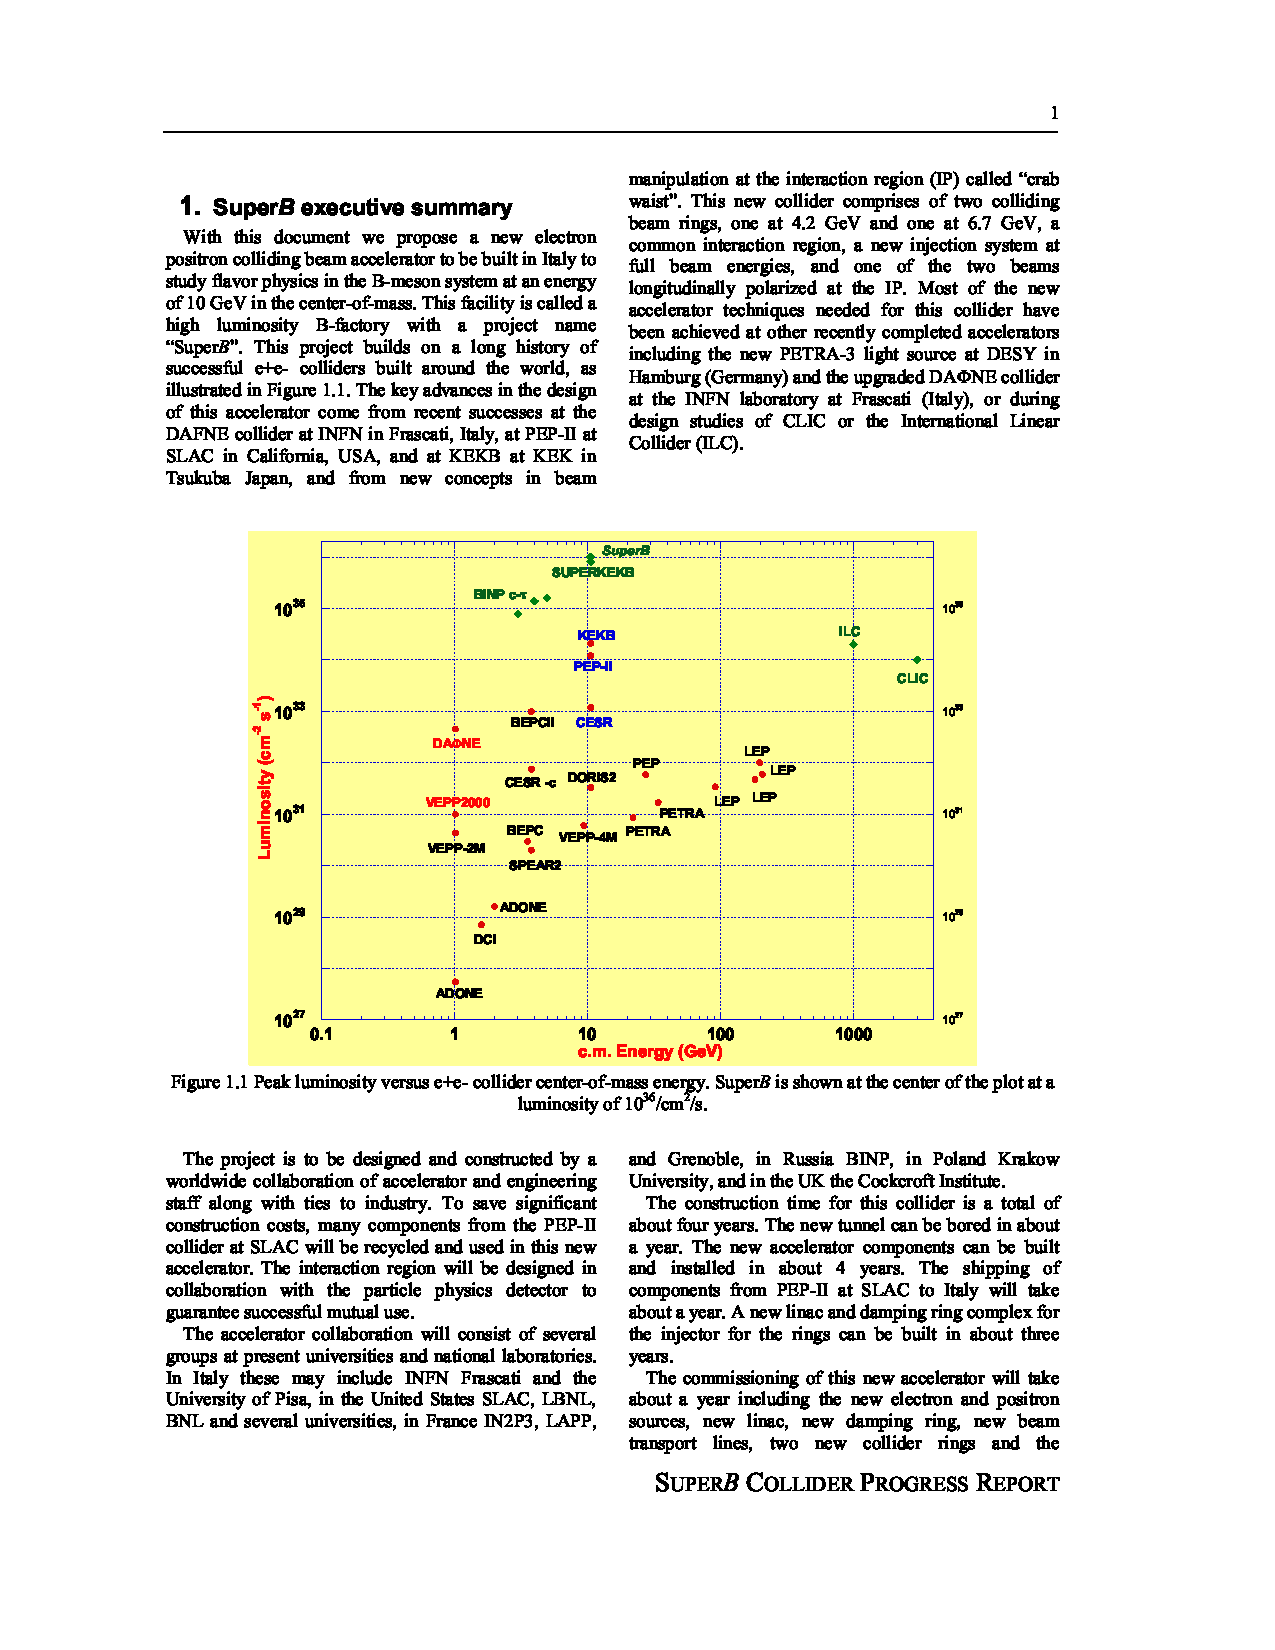
\includegraphics[trim=100 280 150 250,clip=true, scale=0.9]{images/CMvsLum.pdf}
	\caption[Peak luminosity vs centre of mass energy for various collider experiments]{Peak luminosity vs centre of mass energy for various collider experiments~\cite{superbaccelerator}.}	
	\label{fig:CMvsLUM}
\end{figure}

SuperKEKB is a super B-factory which has been built at the KEK high energy laboratory in Tsukuba, Japan. It consists of the SuperKEKB asymmetric \epem collider, storage rings, and the Belle~II detector. The collider will run at a centre of mass energy of 10.58 GeV, which is the mass of the $\Upsilon(4S)$  $b\bar{b}$ resonance. With a luminosity goal of  8$\times10^{35}$ cm$^{-2}$s$^{-1}$, SuperKEKB will be the highest luminosity \epem collider ever built (see Fig \ref{fig:CMvsLUM}).

\section{Physics motivation}

	Electron-positron B-factories are a type of collider experiment that use \epem colliders with high luminosity to make precision measurements of particle interactions involving mesons containing b quark and c quarks as well as tau leptons. Belle~II is a next generation \epem B-factory, called a super-B factory. The centre of mass energy of Belle~II is just enough to produce the $\Upsilon(4S)$ resonance, but the majority of collisions produce other particles, allowing investigation of processes involving charm quarks and tau leptons. Measurements of CP-violation, in which matter and antimatter behave differently, will be made in Belle~II. Due to the precision of the measurements that will be made at Belle~II, small deviations from the Standard Model of particle physics can be detected, which may be a sign of new physics. Searches for other sources of new physics (such as dark matter) are possible through \epem collisions. Rare and forbidden decays can also be measured, which is another sign of new physics~\cite{GrantProp}.


\section{SuperKEKB Collider}
\label{sec:SKB}




SuperKEKB (see Fig \ref{fig:SKB}) is an asymmetric \epem collider built at the KEK high energy laboratory in Tsukuba, Japan. It has been constructed in the same tunnel as its predecessor KEKB, but has many upgrades to increase the luminosity to 8$\times10^{35}$cm$^{-2}$s$^{-1}$, 40 times the luminosity achieved in KEKB. Other beam parameters are presented in Table \ref{tab:SKBBEAM}.

Electrons are produced and accelerated to 7.0 GeV by a linac. Before acceleration, some of the electrons produced are used to generate positrons by irradiation of a tungsten target located in the middle of the linac. Due to the nature of this production, the emittance of the positron beam will be very large. To mitigate this the positron beam will be pulled off the linac and injected into a damping ring. After damping, the positrons are returned to the linac and accelerated to 4.0 GeV. Both rings have a circumference of 3.0 km.

Due to the higher energy of the electron beam, the centre of mass of Belle~II is boosted in the direction that the electron beam is travelling. This boost allows the decay time of the particles produced in the interaction to be dilated by special relativity, enabling time-dependant measurements of CP-violation. 

The electrons and positrons are continuously injected into the high energy ring (HER) and low energy ring (LER). This continuous injection allows the beam current to remain constant, allowing a high luminosity~\cite{BELLE2TDR, ohnishi2013accelerator}.


\begin{table}[htb]
	\centering
	\begin{tabular}{ lcc }
	&	LER	&	HER	\\	\hline \hline
Accelerates	&	e+	&	e-	\\	
Beam Energy (GeV)	&	4.0	&	7.0	\\	
Beam Current (A)	&	3.60	&	2.62	\\	
Horizontal Beam Size ($\mu$m) & 10.2 & 7.75 \\
Vertical Beam Size (nm) & 59  &  59 \\
Number of Bunches	&	\multicolumn{2}{c}{2503}			\\	
Luminosity (cm$^{-2}$s$^{-1}$)	&	\multicolumn{2}{c}{8$\times 10^{35}$}			\\	
Residual beam pipe pressure (nTorr) &  \multicolumn{2}{c}{10}  \\ \hline

	\end{tabular}
	\caption[SuperKEKB beam parameters]{SuperKEKB beam parameters~\cite{BELLE2TDR}.}
	\label{tab:SKBBEAM}
\end{table}



\section{Belle~II detector}

The Belle~II detector is composed of eight subdetectors (see full schematic in Fig \ref{fig:BELLE2}). The inner and outer radii (measured from the beam line axis) as well as the angular acceptance of each subdetector are shown in Table \ref{tab:belleIIaccept}.  Belle~II uses a cylindrical coordinate system to define positions. The $z$-axis runs through the solenoid axis, in the direction that the electron beam travels. Positive $z$ is referred to as the forward direction, and negative $z$ is the backward direction. $x$ is the direction towards the outside of the SuperKEKB ring, and $y$ is upwards. $\phi$ is the azimuthal angle around $z$, and $\theta$ is the zenith angle with respect to $z$.


 This section describes each subdetector, starting at the innermost.

\begin{figure}[htb]
	\centerfloat
		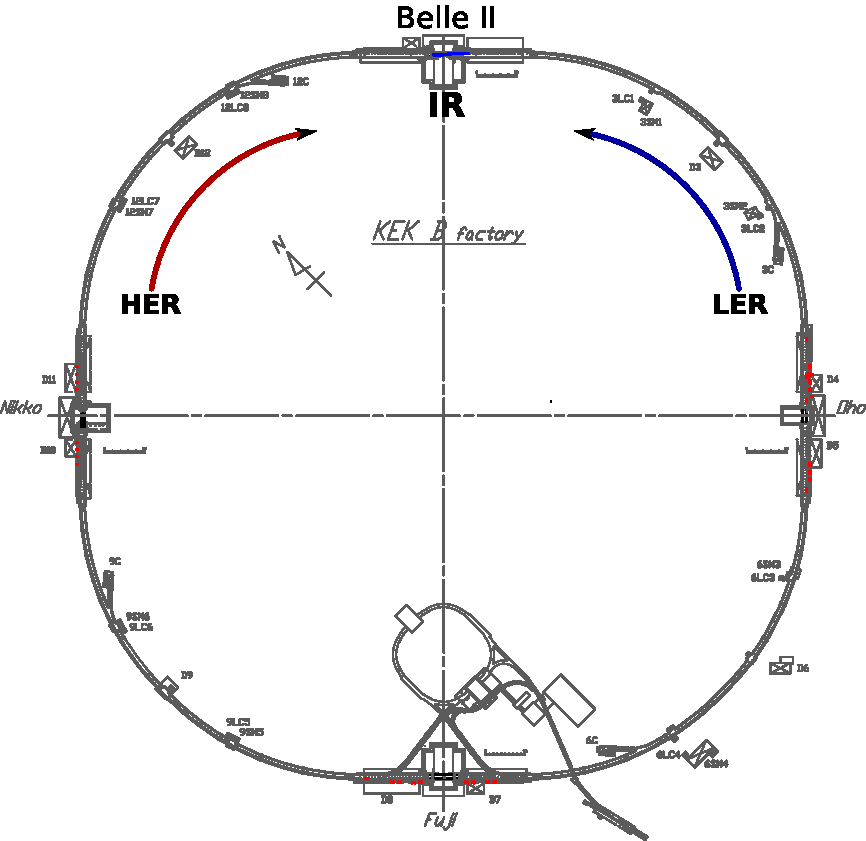
\includegraphics[scale=0.6]{images/SKEKb_key}
	\caption[The SuperKEKB \epem collider]{The SuperKEKB \epem collider. The rings have a circumference of 3 km~\cite{SKBgroup}.}
	\label{fig:SKB}
\end{figure}




\begin{sidewaysfigure}
	\centering
	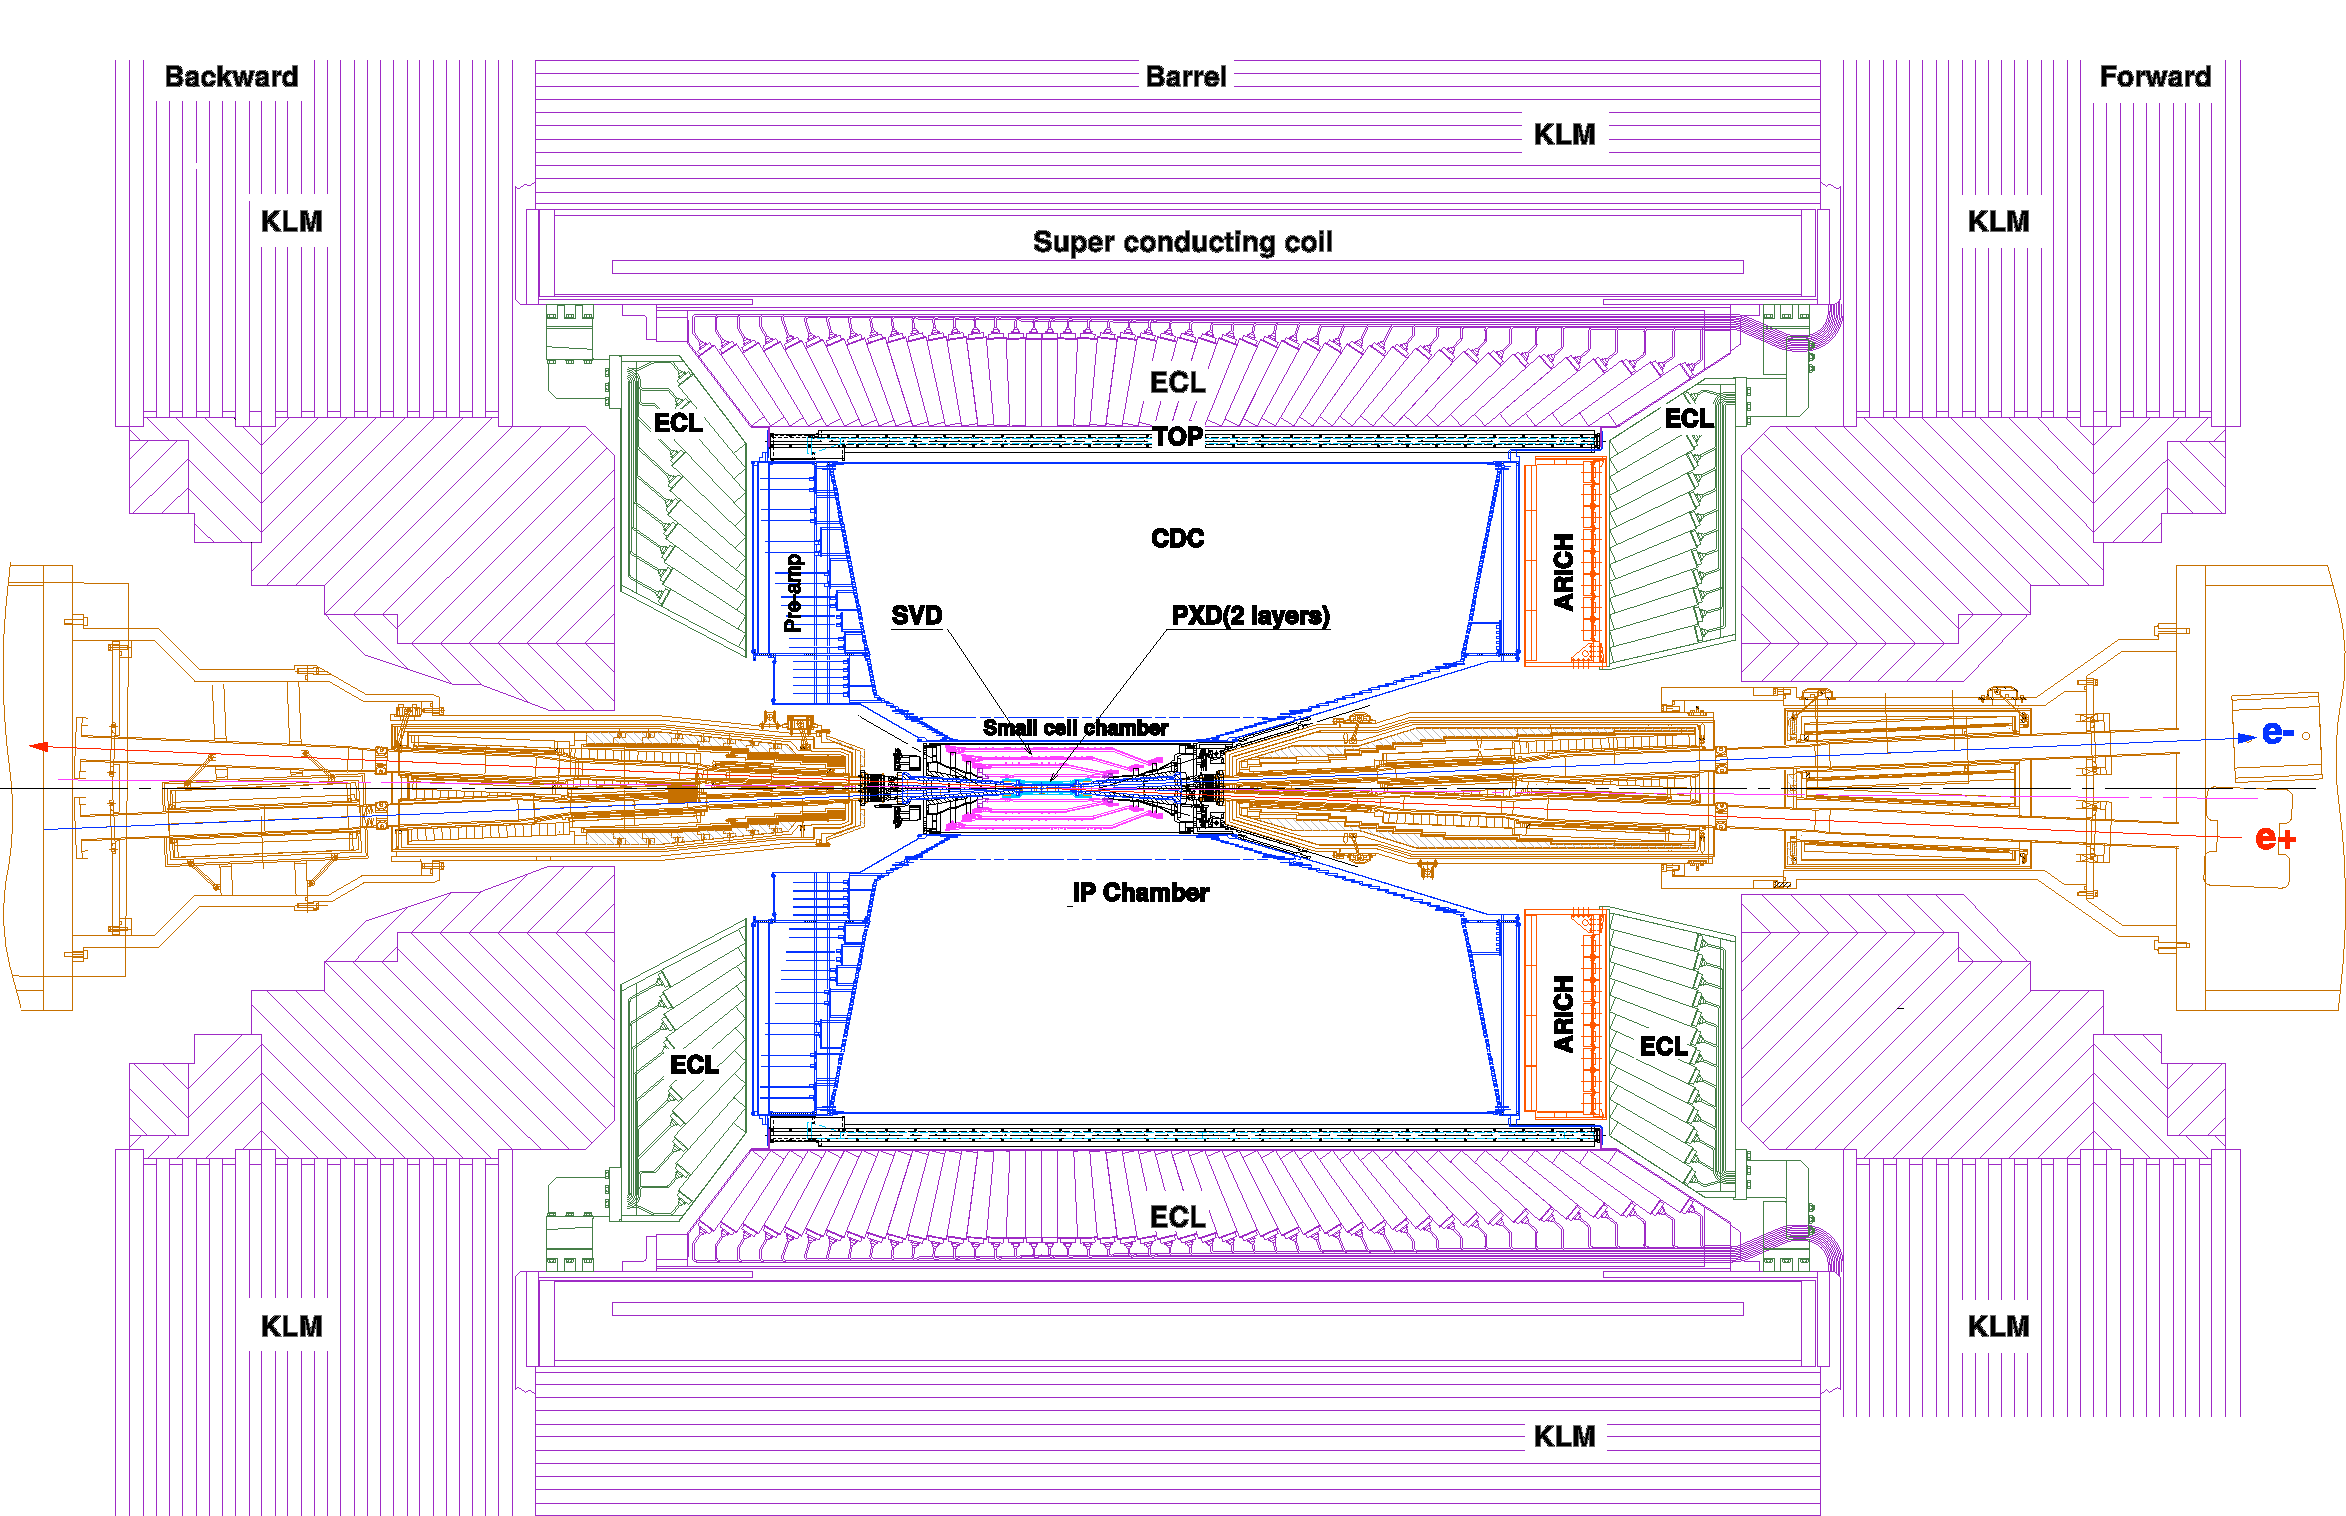
\includegraphics[width=\paperwidth]{images/Belle-llTopview_simple}
	\caption[The Belle~II detector]{Cross section of the Belle~II detector. The forward direction is on the right, and is the direction the electron beam travels. The whole detector is 5 m tall, and approximately symmetric in $\phi$~\cite{BELLE2TDR}.}
	\label{fig:BELLE2}
\end{sidewaysfigure}


\begin{table}[ht]
	\centering
	\begin{tabular}{ lcccc }
Subdetector	&	Inner Radius (mm)	&	Outer Radius (mm)	&	$\theta_{min}$ (deg)	&	$\theta_{max}$ (deg)	\\	\hline \hline
PXD	&	14	&	22	&	17	&	150	\\	
SVD	&	38	&	140	&	17	&	150	\\	
CDC	&	160	&	1130	&	17	&	150	\\	
TOP	&	1190	&	1243	&	32	&	128	\\	
ARICH	&	420	&	1140	&	13	&	34	\\	
Forward ECL	&	1378	&	420	&	12.3	&	32	\\	
Barrel ECL	&	1244	&	1617	&	32	&	130	\\	
Backward ECL	&	417	&	1392	&	130	&	155.1	\\	
BKLM	&	1952	&	2475	&	45	&	125	\\	
EKLM	&	1248	&	2475	&	20	&	145	\\	\hline

	\end{tabular}
	\caption[Inner and outer radii, and angular acceptances of Belle~II subdetectors]{Inner and outer radii, and angular acceptances of Belle~II subdetectors, measured from the forward direction. The detectors are approximately symmetric in $\phi$.}
	\label{tab:belleIIaccept}
\end{table}



\subsection{Vertex Detector}
\label{sec:VXD}

	Belle~II's vertex detector (VXD) is made up of two tracking subdetectors. The inner detector is the pixel detector, which is surrounded by the silicon vertex detector.

\subsubsection{Pixel Detector}
\label{sec:PXD}

	The \textbf{P}i\textbf{X}el \textbf{D}etector (PXD) is wrapped around the beampipe. This subdetector is made up of two cylindrical layers containing solid state pixel cells. The inner cylinder has a radius of 1.4 cm and has eight segments, while the outer cylinder has a radius of 2.2 cm and has 12 segments. The PXD contains about 8 million individual pixel cells \cite{BELLE2TDR, schieck2013depfet}.


\subsubsection{Silicon Vertex Detector}
\label{sec:SVD}

	The \textbf{S}ilicon \textbf{V}ertex \textbf{D}etector (SVD) surrounds the PXD. Its purpose is to measure decay vertices, particularly those of B decays. It consists of four layers containing strips of double sided silicon detectors. Due to the smaller Lorentz boost of Belle~II compared to Belle, there is less separation between the B decay vertices; however, the beampipe of Belle~II is smaller, which allows the Belle~II SVD to have improved performance compared to Belle \cite{BELLE2TDR}.

	


\subsection{Central Drift Chamber}
\label{sec:CDC}

	The \textbf{C}entral \textbf{D}rift \textbf{C}hamber (CDC) surrounds the VXD. It provides three important functions: reconstruction of tracks and momentum measurements of charged particles, particle identification through energy loss within the gas volume, and efficient and reliable triggers for charged particle tracks. The CDC is a cylindrical chamber, with over 14,000 sense wires strung along the length of the cylinder. It is filled with He-C$_2$H$_6$. As charged particles traverse the gas, they create tracks of ionization, which are detected by the sense wires. The path of the particle through the CDC can then be reconstructed. The CDC is immersed in a 1.5~T solenoidal magnetic field, parallel to the beampipe. This allows the CDC to act as a large magnetic spectrometer ~\cite{BELLE2TDR}.


\subsection{Particle ID}
\label{sec:PAID}

	Belle~II has two particle ID (PID) detectors: the TOP and the ARICH. The TOP is in the central region of Belle~II, while the ARICH is in the forward region.

\subsubsection{Time of Propagation Counter}
\label{sec:TOP}

	The barrel PID detector is known as the \textbf{T}ime \textbf{O}f \textbf{P}ropagation (TOP) counter. Its purpose is to improve Belle~II's ability to distinguish between kaons and pions. The counter measures the time of propagation of Cherenkov photons internally reflected within a quartz radiator. The detector consists of 16 modules which run parallel to the axis of Belle~II. Each module is made up of a single rectangular bar of quartz with a focusing mirror on one end and a photomultiplier tube (PMT) on the other end. As particles traverse the crystal, Cherenkov light is produced in the crystal. This light is reflected down the bar into the PMT. Information about the incident particle's ID can be inferred from this light~\cite{BELLE2TDR}.


\subsubsection{Aerogel Ring-Imaging Cherenkov detector}
\label{sec:ARICH}

	Sandwiched between the CDC and the forward ECL end-cap is the \textbf{A}erogel \textbf{R}ing-\textbf{I}maging \textbf{CH}erenkov (ARICH) detector. Its purpose is to identify kaons and pions over most of the momentum range and to discriminate between pions, muons, and electrons at momenta below 1 GeV/c. The detector consists of an aerogel radiator where charged particles create Cherenkov photons, an expansion volume where the photons propagate so that distinctly measurable rings can form, and an array of photon detectors (known as HAPDs: \textbf{H}ybrid \textbf{A}dvanced \textbf{P}hoto-\textbf{D}etector) which measure the Cherenkov rings~\cite{BELLE2TDR}.



\subsection{Electromagnetic Calorimeter}
\label{sec:ECL}

	The \textbf{E}lectromagnetic \textbf{C}alorimeter (ECL) has several tasks: high efficiency photon detection, precise photon energy and angular measurements, identification of electrons, trigger signalling, luminosity measurements, and (with the $K_{L}^0$ and $\mu$ detector) K$_L^0$ measurement. Note that all particles will potentially lose some energy that is measured in the ECL, which will contribute to particle identification. The ECL is composed of 8,736 crystals of thallium doped caesium iodide (CsI(Tl)) and is divided into three parts: the forward end-cap containing 1,152 crystals, the barrel containing 6,624 crystals, and the backward end-cap containing 960 crystals. Apart from the electronics the entire calorimeter is the same as was used in the Belle experiment. Each crystal is roughly 30~cm in length, which corresponds to 16 radiation lengths. The crystals have a cross section of $\sim5~\mathrm{cm}\times5~\mathrm{cm}$.

Attached to the end of each crystal is a diode that measures the scintillation light produced by the crystal, which is proportional to the energy deposited in that crystal. The front-end electronics of the ECL have been upgraded since Belle and now read and process the waveforms using a Field Programmable Gate Array (FPGA), producing time and amplitude \cite{BELLE2TDR}.


\subsection{K$_L^0$ and $\mu$ detector}
\label{sec:KLM}


The outermost detector system is the K$_L^0$ and $\mu$ detector (KLM), which is made of three components: two end-caps (EKLM) and a barrel (BKLM). These components consist of alternating layers of 4.7~cm thick iron plates and active detector material. In the barrel, the active material is made up of glass-electrode resistive plate chambers (RPC). The end-caps have to deal with a much higher background flux, so the active materials there are scintillators. The barrel KLM covers 45$^{\circ}$ to 125$^{\circ}$ and is made up of 15 layers, providing 3.9 interaction lengths of material. The end-caps extend this range from 20$^{\circ}$ to 155$^{\circ}$. The forward end-cap has 12 layers, while the backward end-cap has 14 layers~\cite{BELLE2TDR}.

\subsection{Shielding}

	In order to mitigate the effects of beam backgrounds, shields composed of polyethylene with 5\% boron and lead are installed inside the forward and backward ECL. The polyethylene and boron absorb neutrons and the lead absorbs photons and electrons. In addition to this, the ARICH has a small neutron shield made of polyethylene built into it.

\subsection{Neutron Damage to Belle~II Subdetectors}



	The readout electronics of each subdetector are all silicon based. 3.05\% of silicon is composed of the $^{30}$Si isotope, which can be transmuted into phosphorous by this reaction:
\begin{equation}
	{^{30}\mathrm{Si} + \mathrm{n}\rightarrow~^{31}\mathrm{Si}+\gamma \rightarrow~^{31}\mathrm{P}+\beta^{-}+\gamma}
\end{equation}
which introduces an n-type dopant into the silicon, altering its electronic properties. Additionally, there is lattice damage caused by recoil. Other silicon isotopes, $^{28}$Si and $^{29}$Si will also absorb neutrons, but since they remain silicon, they do not alter the electronic properties other than introducing lattice damage~\cite{young1978radiation}.

The simulated neutron flux in each Belle~II subdetector is presented in Chapter~\ref{chap:Conseqences}. The unscaled figures are for the basic simulation and the scaled figures are after the analysis presented in this dissertation. Expected neutron fluxes are on the order of $10^9$ neutrons cm$^{-2}$yr$^{-1}$ for most detectors, with the vertex detectors having a higher flux, and the KLM detectors having a lower flux. Some detectors are more sensitive to neutron background, particularly the ARICH and TOP detectors and the electronic components of the other detector readouts.




%Several subdetectors are particularly sensitive to neutron damage: the ARICH and the TOP. 

%ARICH: Noise increases. Has additional shielding

















\chapter{BEAST~II}
\label{chap:BEASTDet}


%Before the Belle~II detector is rolled in

\section{Overview}

	Beam backgrounds (discussed in detail in Chapter \ref{chap:beamBack}) are an important consideration in any collider experiment. Simulations of these backgrounds are calculated (discussed in Chapter \ref{chap:Sim}) to ensure that these backgrounds will not damage the sensitive components of Belle~II. It is important to make measurements of the backgrounds as well, to determine the level of accuracy of the simulations. This is the purpose of BEAST~II (\textbf{B}eam \textbf{E}xorcism for \textbf{A} \textbf{S}table experimen\textbf{T}). The \he tube and CsI detector systems are especially geared toward verification of the simulation.

	BEAST~II consists of three distinct phases. Phase~I consists of a skeletal framework with several subdetectors, shown in Fig \ref{fig:beastRender}, all covered by a concrete shield. Table \ref{tab:beastPhase1} lists the subdetectors in Phase~I. In Phase~II, the Belle~II detector will be wheeled in (without the VXD system), with several subdetectors from Phase~I in place. In Phase~III, the VXD will be installed and the transition from background measurement to full physics running will begin.

	The focus of this dissertation is Phase~I, where only beam-gas and Touschek backgrounds are present and therefore more easily measured. A description of the various components of this phase follows.

\begin{figure}[htb]
	\centerfloat
		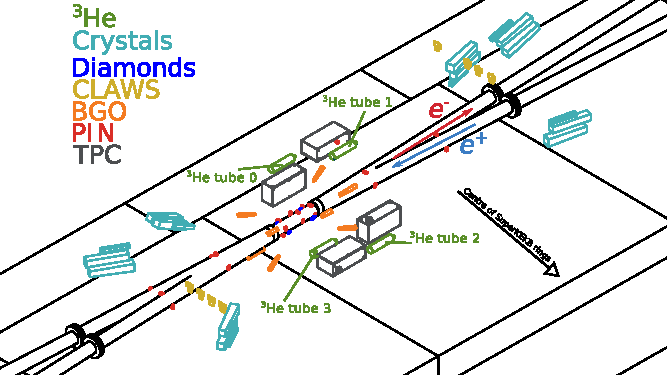
\includegraphics[width=\textwidth]{images/BEAST-Phase1-LineArt-16-9_IsoMetric-Colours-EmbeddedText}
	\caption[CAD rendering of BEAST~II in Phase~I]{CAD rendering of BEAST~II showing colour-coded locations of all subdetectors. The support structure is omitted for clarity~\cite{BEASTPAPER}.}
	\label{fig:beastRender}
\end{figure}

%\begin{figure}[ht!]
%\centering
%%% Creator: Inkscape 0.91_64bit, www.inkscape.org
%% PDF/EPS/PS + LaTeX output extension by Johan Engelen, 2010
%% Accompanies image file 'BEAST-Phase1-MasterCoordinateSystem-v2.pdf' (pdf, eps, ps)
%%
%% To include the image in your LaTeX document, write
%%   \input{<filename>.pdf_tex}
%%  instead of
%%   \includegraphics{<filename>.pdf}
%% To scale the image, write
%%   \def\svgwidth{<desired width>}
%%   \input{<filename>.pdf_tex}
%%  instead of
%%   \includegraphics[width=<desired width>]{<filename>.pdf}
%%
%% Images with a different path to the parent latex file can
%% be accessed with the `import' package (which may need to be
%% installed) using
%%   \usepackage{import}
%% in the preamble, and then including the image with
%%   \import{<path to file>}{<filename>.pdf_tex}
%% Alternatively, one can specify
%%   \graphicspath{{<path to file>/}}
%% 
%% For more information, please see info/svg-inkscape on CTAN:
%%   http://tug.ctan.org/tex-archive/info/svg-inkscape
%%
\begingroup%
  \makeatletter%
  \providecommand\color[2][]{%
    \errmessage{(Inkscape) Color is used for the text in Inkscape, but the package 'color.sty' is not loaded}%
    \renewcommand\color[2][]{}%
  }%
  \providecommand\transparent[1]{%
    \errmessage{(Inkscape) Transparency is used (non-zero) for the text in Inkscape, but the package 'transparent.sty' is not loaded}%
    \renewcommand\transparent[1]{}%
  }%
  \providecommand\rotatebox[2]{#2}%
  \ifx\svgwidth\undefined%
%    \setlength{\unitlength}{229.9bp}%
    \setlength{\unitlength}{\textwidth}	
    \ifx\svgscale\undefined%
      \relax%
    \else%
      \setlength{\unitlength}{\unitlength * \real{\svgscale}}%
    \fi%
  \else%
    \setlength{\unitlength}{\svgwidth}%
  \fi%
  \global\let\svgwidth\undefined%
  \global\let\svgscale\undefined%
  \makeatother%
  \begin{picture}(1,1)%
    \put(0,0){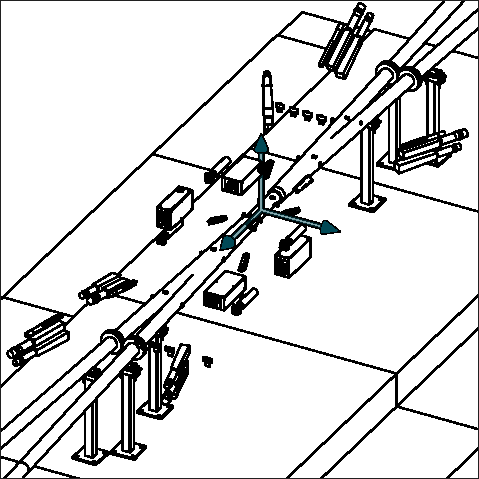
\includegraphics[width=\unitlength,page=1]{images/BEAST-Phase1-MasterCoordinateSystem-v2.pdf}}%
    \put(0.43004132,0.49912999){\color[rgb]{0       , 0.282353, 0.333333} $z$}%
    \put(0.67935308,0.47502588){\color[rgb]{0       , 0.282353, 0.333333} $x$}%
    \put(0.56545083,0.68934171){\color[rgb]{0       , 0.282353, 0.333333} $y$}%
    \put(0,0){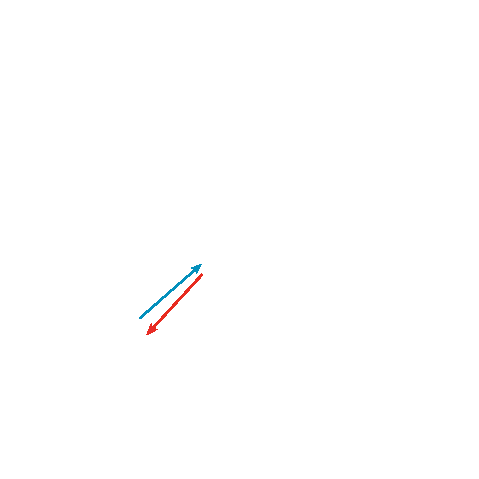
\includegraphics[width=\unitlength,page=1]{images/BEAST-Phase1-MasterCoordinateSystem-Arrows.pdf}}%
    \put(0.3617227,0.3072984){\color[RGB]{232,44,42}$e^{-}$}%
    \put(0.31324316,0.40748951){\color[RGB]{4,144,188}$e^{+}$}%
  \end{picture}%
\endgroup%

%\caption[CAD render of BEAST~II in Phase~I]{CAD render of BEAST~II showing locations of all subdetectors. Support structure is omitted for clarity}
%\label{fig:beastRender} ~\cite{BEASTPAPER}
%\end{figure}


\begin{table}[ht]
	\centering
	\begin{tabular}{ llc }
		Subdetector	&	Purpose				&	Number of devices	\\	\hline \hline
		PINs		&	Ionizing radiation		&	64	\\	
		Crystals	&	Injection and 
					Machine backgrounds		&	18	\\	
		\He tubes	&	Thermal neutron detection	&	4	\\	
		Time projection
		 chambers	&	Fast neutron detection		&	2	\\	
		CLAWS		&	Fast injection background	&	8	\\	
		Diamonds	&	Radiation dose monitor		&	4	\\	
		BGO		&	Machine backgrounds		&	8	\\	\hline
	\end{tabular}
	\caption[Summary of BEAST~II Phase~I detectors]{Summary of BEAST~II Phase~I detectors.}
	\label{tab:beastPhase1}
\end{table}


\section{Crystals}
\label{sec:CSI}

	The crystal subsystem consists of six crystal boxes, three on each side of the interaction region (IR). Each box contains three crystals: pure caesium iodide (CsI), thallium doped CsI (CsI(Tl)), and cerium-doped lutetium yttrium orthosilicate (LYSO). When charged particles enter these crystals, they generate showers and produce visible light with an intensity proportional to the energy deposited by the particle. Photomultiplier tubes attached to the end of the crystals collect this light and produce a signal.


\section{BGO}

	Eight bismuth germanate (\textbf{B}i$_4$\textbf{G}e$_3$\textbf{O}$_{12}$ - BGO) crystals (four in the forward region, four in the backward region) are installed with their long axes pointing at the interaction point (IP). In Phase~II of BEAST~II, these will measure the radiative Bhabha events. In Phase~I, they act as a general monitor of radiation. The BGO crystals measure radiation in the same way as the crystals discussed in \S~\ref{sec:CSI}. 

\section{TPCs}
\label{sec:TPCs}
	
	The fast neutron \textbf{T}ime \textbf{P}rojection \textbf{C}hambers (TPCs) detect fast neutrons by measuring tracks from recoiling alpha particles. The detectors themselves are rectangular boxes filled with helium. When the alpha particles recoil, they produce ionization tracks which drift to a sensor at the end of the box. There were four TPCs in place in Phase~I of BEAST~II, two of which were operating. 



\section{Diamonds}

	Four $(4.5\times4.5\times0.5$mm$)^2$ diamond sensors are mounted to the beampipe near the IR. The purpose of these sensors is to provide an instantaneous and integrated measurement of the dose near the IR. The diamond crystals have electrodes deposited on opposite sides. A potential difference applied between the electrodes produces an electric field of approximately 1 V/$\mu $. When charged particles cross the diamond, an electron-hole pair is produced for each 13 eV of energy that is deposited. These electron-hole pairs produce a current in the diamond, which is measured to determine the dose.


\section{PINs}

	An array of PIN (three layers of semiconductor: \textbf{P}-doped, \textbf{I}ntrinsic, and \textbf{N}-doped) diodes at various locations around BEAST~II provide a simple and inexpensive measurement of ionizing radiation. The radiation produces an increase in the dark current of the diodes, which is measured to provide the dose. Half of the PIN diodes are coated in a thin layer of gold paint, which reduces the X-ray dose. A comparison between shielded and unshielded diodes gives a direct measurement of the syncrotron radiation dose. Each PIN subdetector contains two diodes (one gold coated, and one not) and a temperature monitor encased in an aluminum block. Eight sets of four blocks are placed at various locations surrounding the beampipe, for a total of 64 channels.

\section{CLAWS}

	The s\textbf{C}intillation \textbf{L}ight \textbf{A}nd \textbf{W}aveform \textbf{S}ensors (CLAWS) detector system measures backgrounds, in particular those caused by injection. It consists of eight scintillator tiles read out by silicon photomultipliers. The system has a 0.8 ns sampling rate, making it ideal for measuring the fast injection signals. These results are sent to the SuperKEKB control room, providing fast feedback of accelerator performance.


\section{\He Tubes}

	The \he tubes provide thermal neutron detection, and are discussed in detail in Chapter \ref{chap:he3tube}.


\section{Phase~II}

	In the fall of 2017, Phase~II of BEAST~II will begin. During this phase, the Belle~II detector (without the VXD systems) will be rolled into the IR. Phase~I devices will continue to be used in this phase, with the exception of the crystal boxes, as the ECL will take similar measurements. In addition, there will be two new subdetectors: \textbf{F}E-I4 \textbf{A}TLAS \textbf{N}ear \textbf{G}amma \textbf{S}ensors (FANGS) and \textbf{P}ixelated \textbf{L}adder with \textbf{U}ltra-low \textbf{M}aterial \textbf{E}mbedding (PLUME). The CLAWS, FANGS, PLUME, and BGO systems will be installed in the VXD space. The TPCs and \he tubes will go into the dock spaces as shown in Fig \ref{fig:dockSpace}. During this phase, the 1.5 T magnetic field of Belle~II will be turned on.

\begin{figure}[htb]
	\centerfloat
		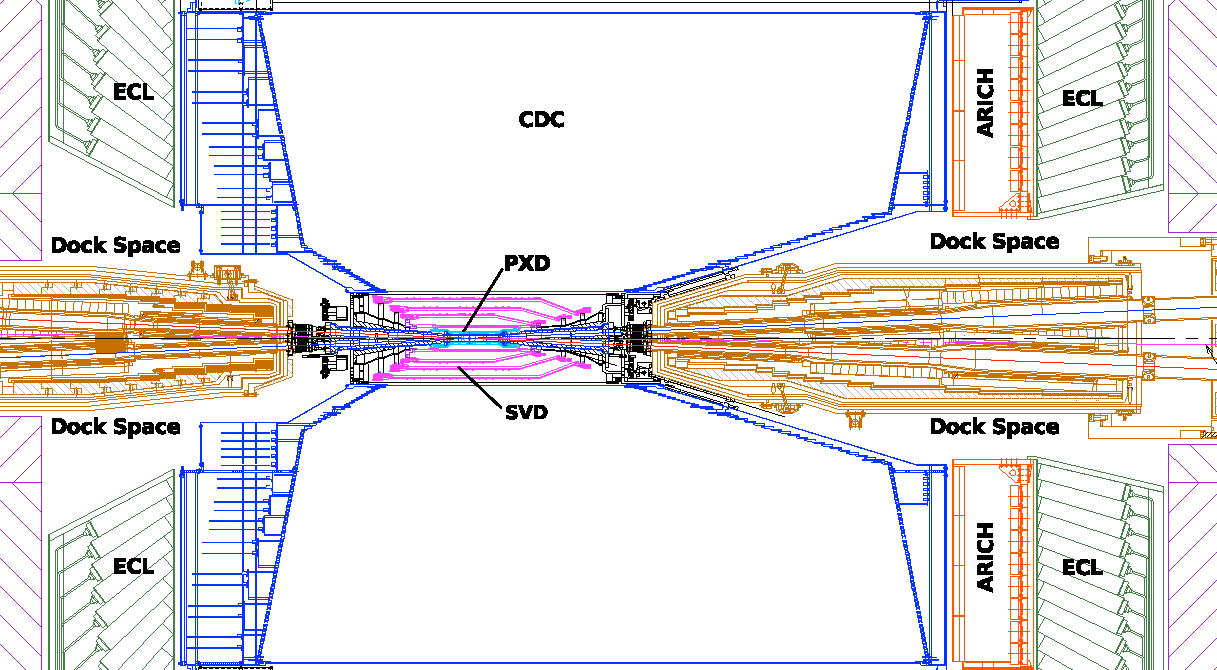
\includegraphics[width=\textwidth]{images/Belle-ll-DockSpace_text}
	\caption[Belle~II dock spaces]{Belle~II dock spaces.}		
	\label{fig:dockSpace}
\end{figure}




















\chapter{\He Tubes}
\label{chap:he3tube}

\section{Description}


\begin{figure}[htb]
	\centerfloat
		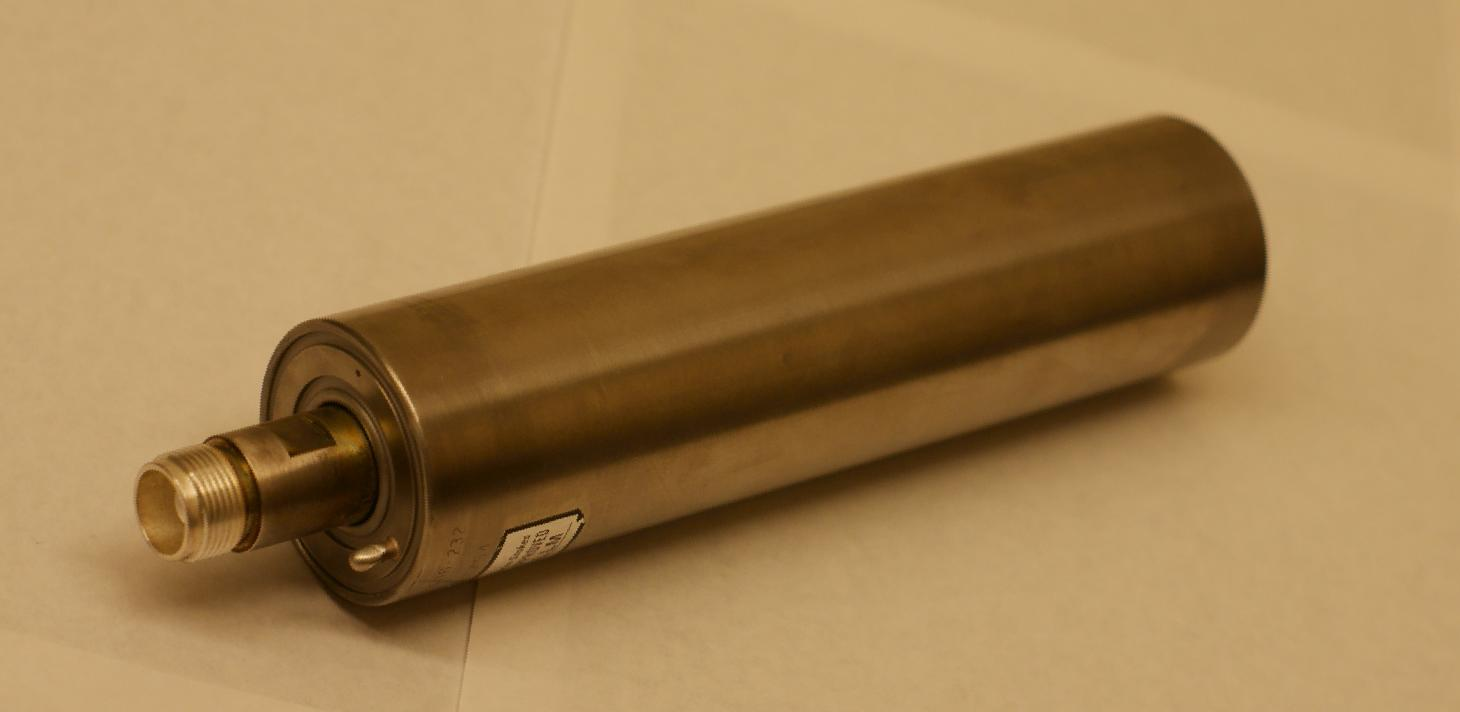
\includegraphics[scale=0.25]{images/he3tubePhoto}
	\caption[\He tube]{\He tube (see Fig~\ref{fig:he3spec} for a detailed schematic of the detector).}
	\label{fig:he3photo}
\end{figure}

	Four \he tubes were procured from GE-Reuter Stokes for the purpose of thermal neutron detection in BEAST~II. They consist of stainless steel tubes 9.47$^{\verb+"+}$ long and 2$^{\verb+"+}$ in diameter filled with $^3$He at 4 atm of pressure. 


\section{Theory of Operation}

When a thermal neutron (with an energy of 0.025 eV) passes through the active area of the detector, it may be captured by a $^3$He atom~\cite{Oed200462}:

\begin{equation}
		{^{3}_{2}\mathrm{He}+^{1}_{0}\mathrm{n}\rightarrow~^{3}_{1}\mathrm{H}+^{1}_{1}H+764~\mathrm{keV}}
\end{equation}

The cross section for this reaction decreases as the energy of the neutron increases, as shown in Fig~\ref{fig:neutCross}. The $^3$H and proton ionize the gas in the tubes. This ionization produces a signal on a sense wire in the centre of the tube.

	The signal is read out by a custom amplifier system designed and built by the electronics shop at the University of Victoria. 


\begin{figure}[htb]
	\centerfloat
		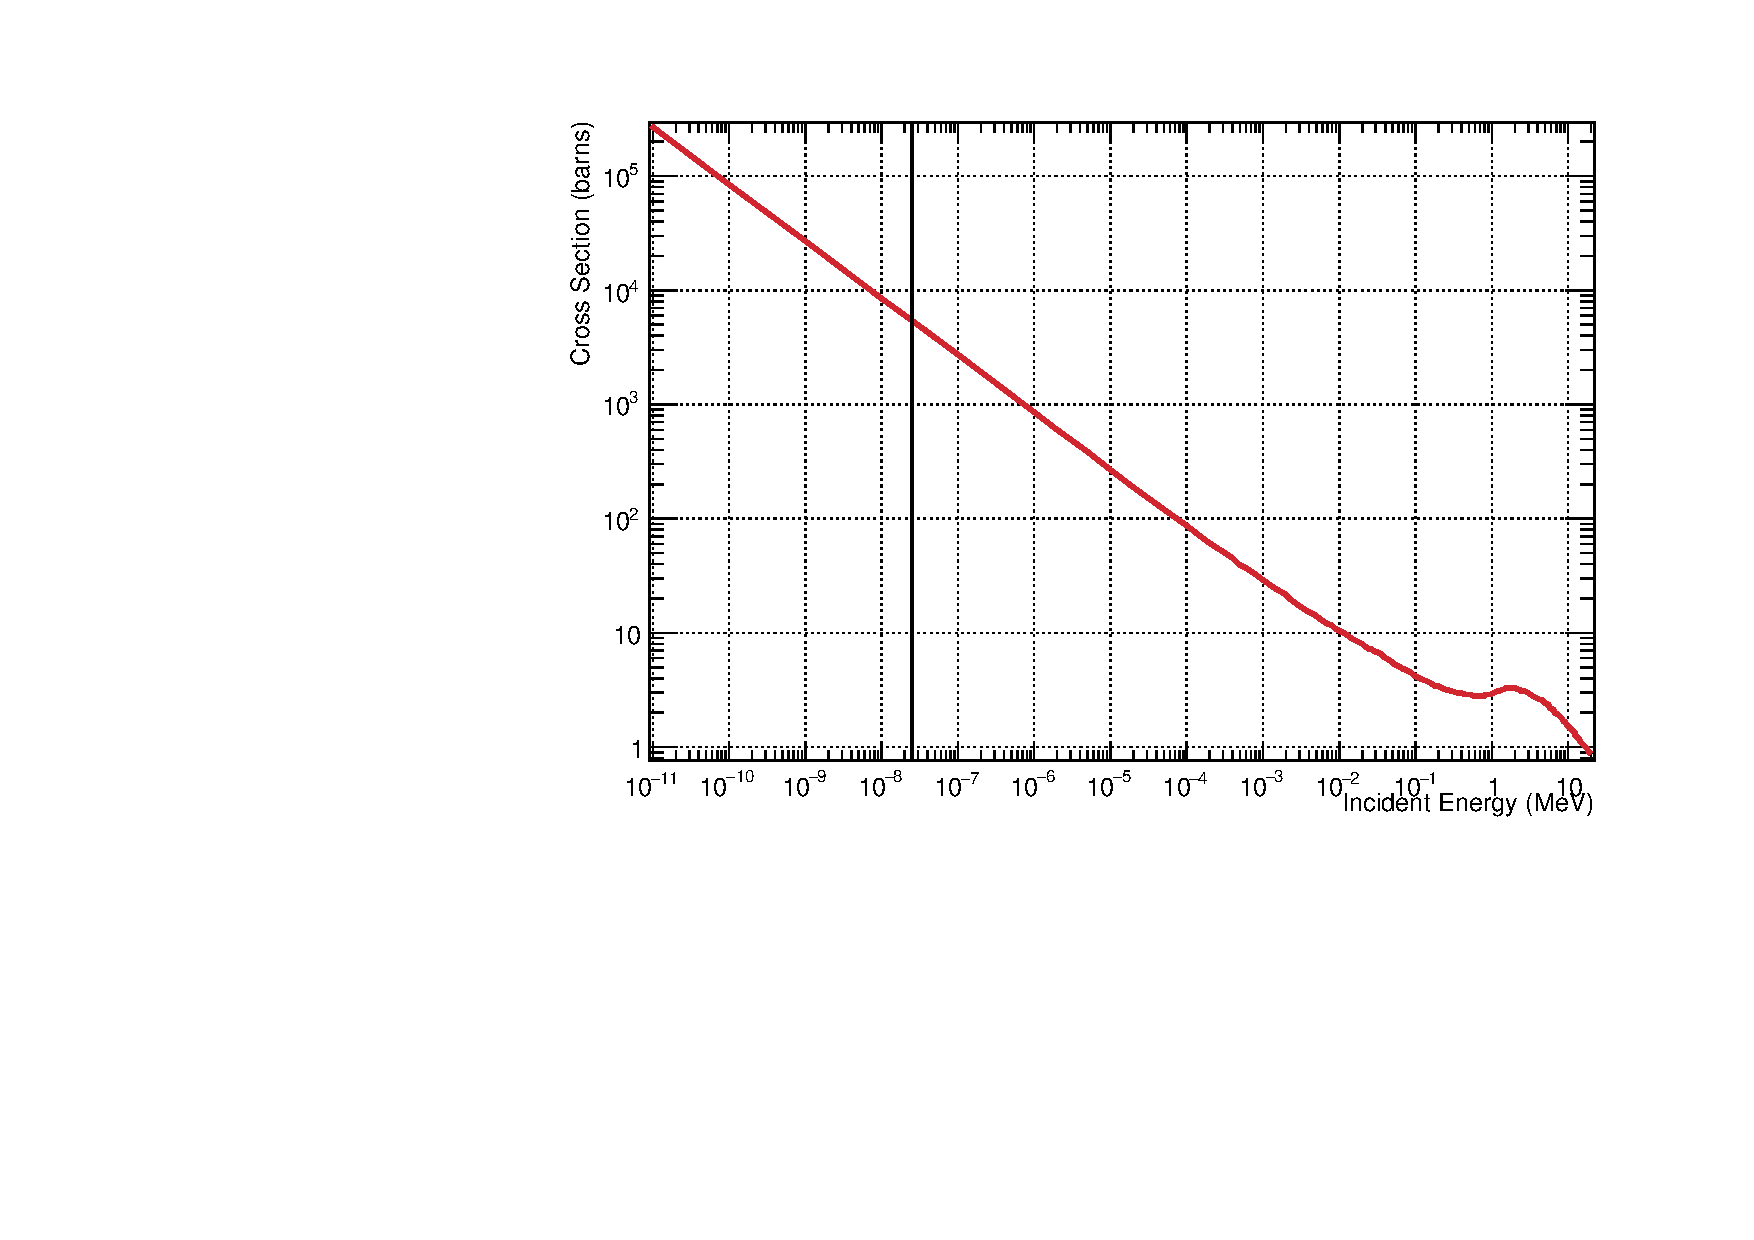
\includegraphics[width=\textwidth]{images/neutron_cross_section}
	\caption[Cross section of neutron capture by \he as a function of neutron energy]{Cross section of neutron capture by \he as a function of neutron energy. The vertical black line corresponds to upper range of the energy of thermal neutrons~\cite{BNL}.}
	\label{fig:neutCross}
\end{figure}


\section{Readout Electronics}

	The \he tube amplification system consists of two devices: an amplifier module that is attached directly to the back end of the tube (see Figs~\ref{fig:he3ampfront} and~\ref{fig:he3ampread}), and a receiver box that plugs into a slot in a NIM crate (see Fig~\ref{fig:he3Rec}). Both of these devices were designed and built in the electronics shop in the physics department at the University of Victoria.

\begin{figure}[htb]
    \centering
    \begin{tabular}{ccc}
	\subfigure[Amplifier Front]{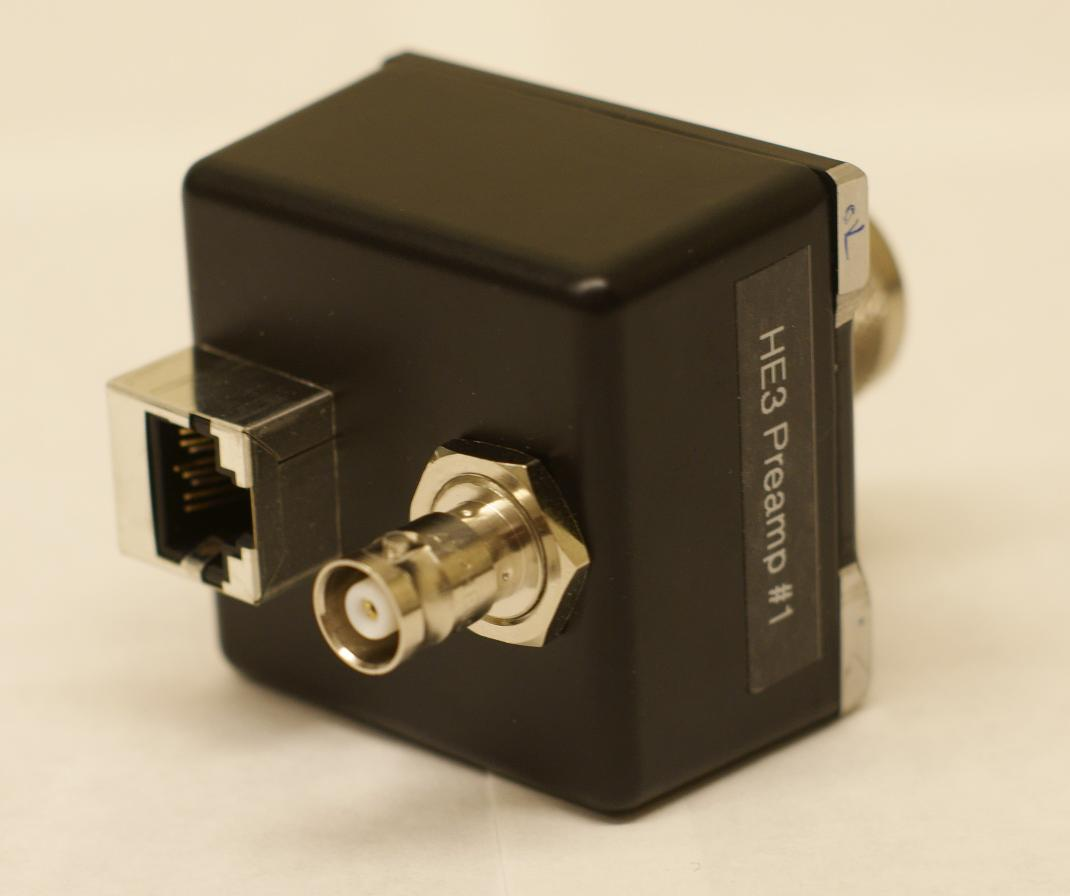
\includegraphics[scale=0.12]{images/preampPhoto}\label{fig:he3ampfront}} & 
	\multirow{-3}[18]{*}{\subfigure[Receiver box]{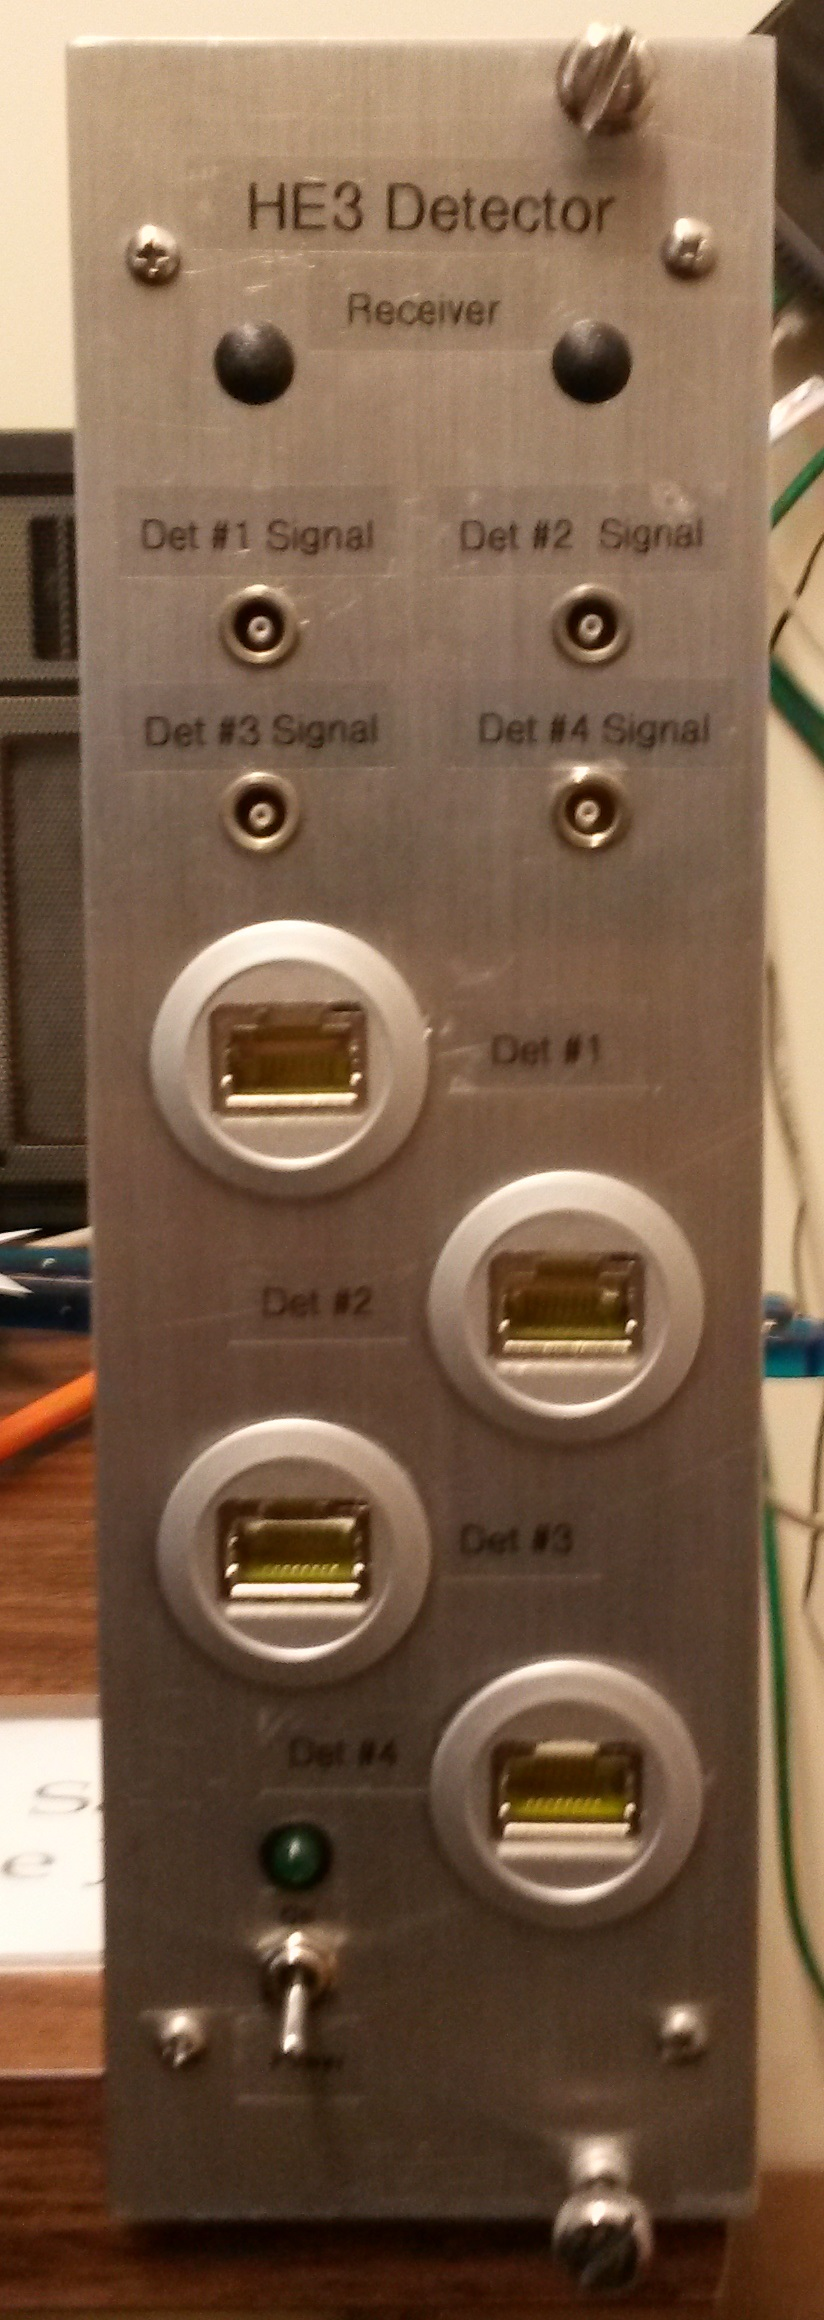
\includegraphics[height=6.2cm]{images/RecieverBoxPhoto}\label{fig:he3Rec}}} &
	\multirow{-3}[18]{*}{\subfigure[Power supply]{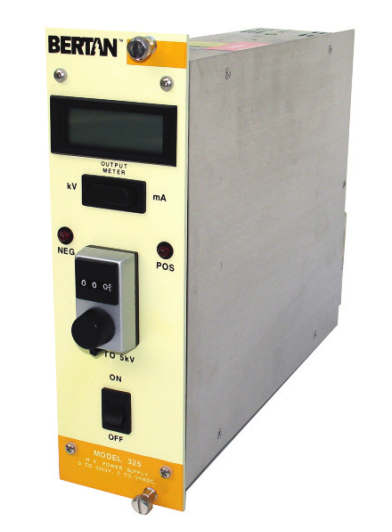
\includegraphics[height=6.2cm]{images/bertan}\label{fig:he3HV}}} \\
	\subfigure[Amplifier Rear]{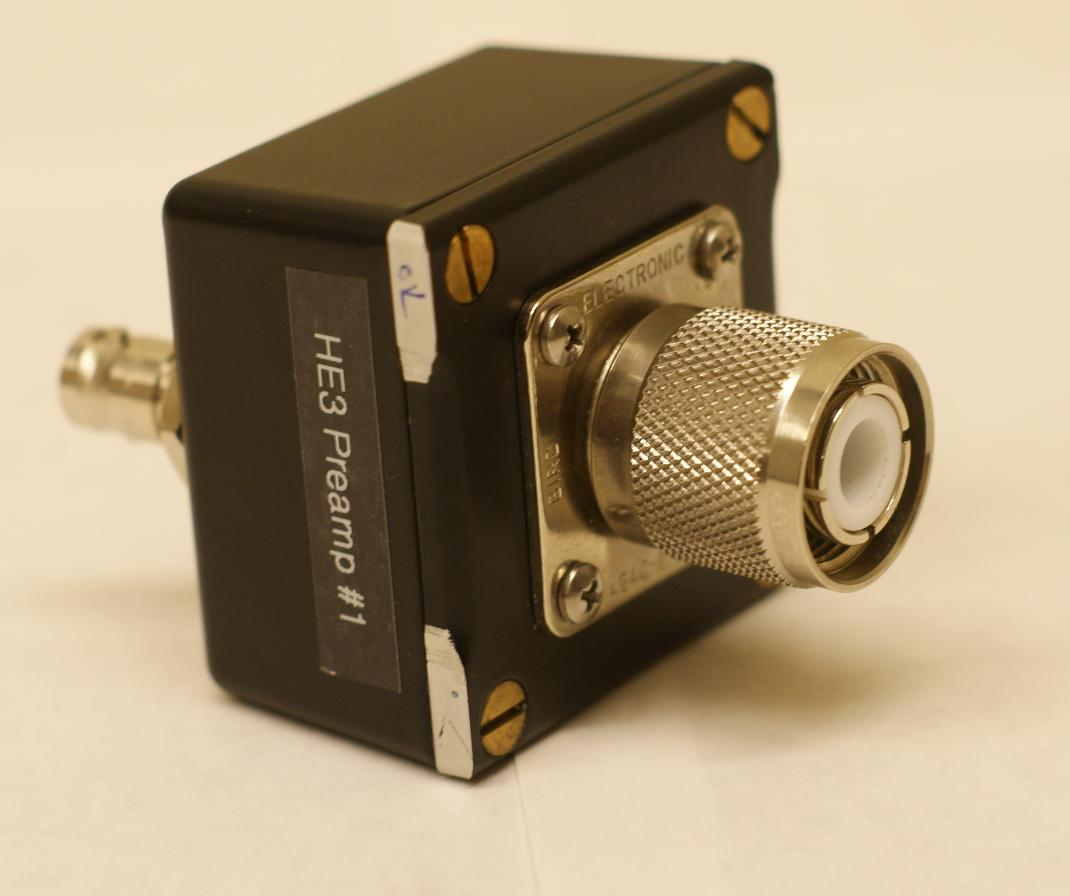
\includegraphics[scale=0.12]{images/preampPhoto2}\label{fig:he3ampread}}\\
    \end{tabular}
    \caption[Amplifier module, receiver box, and power supply]{Amplifier module, receiver box, and power supply. Circuit diagrams can be found in Appendix~\ref{chap:he3spec}.}
    \label{fig:he3ampRec}
\end{figure}


\subsection{Amplifier Module}

	The amplifier module is attached to the end of the \he tube. It is connected to the sense wire of the \he tube via a 47~pF capacitor to remove the high voltage (HV) on the sense wire. This amplifier provides a gain of 2. Once the signal is amplified, it is sent through a differential line driver. The signal is split into two identical components, one of which has its polarity reversed. These signals are then sent down a twisted pair CAT-6 cable. Low voltage power for the amplifier circuitry is also provided by the CAT-6 cable. A circuit diagram can be z~\ref{fig:he3preampLineDriver}~\cite{Honkanen}.

	In addition to amplifying the \he tube signal, the amplifier module also routes high voltage of 1.58~kV to the sense wire in the tube. This high voltage is produced by a Bertan model 323 HV power supply (see Fig~\ref{fig:he3HV}).


\subsection{Receiver Box}

	The receiver box contains integrated circuits (ICs) which receive the signal from the CAT-6 cable, and provides the low voltage to power the amplifier circuit in the amplifier modules. The split signal from the amplifier is combined at the receiver box. This differential signal approach should reduce most electronic noise, since the noise should affect both the inverted signal and the non-inverted signals and any noise which affects both will be removed when the two are combined. The receiver box outputs the signals via lemo connections on the front. The box contains four separate ICs, and as such can handle the signals from four different tubes. It is powered by the NIM back plane. A circuit diagram can be found in Fig~\ref{fig:he3LineReciever}~\cite{Honkanen}.



\section{Data Acquisition}

	Data acquisition (DAQ) is performed with a CAEN 1724 digitizer (Fig~\ref{fig:CAENDIGI}). This device receives the signals from the receiver box and records the pulse height and time of a signal waveform, with a time resolution of 20 ns. This information is then passed to a computer via a VME-USB bridge (Fig~\ref{fig:CAENCON}).


\begin{figure}[htb]
    \centering
    \begin{tabular}{cc}
	\subfigure[V1724 Digitizer]{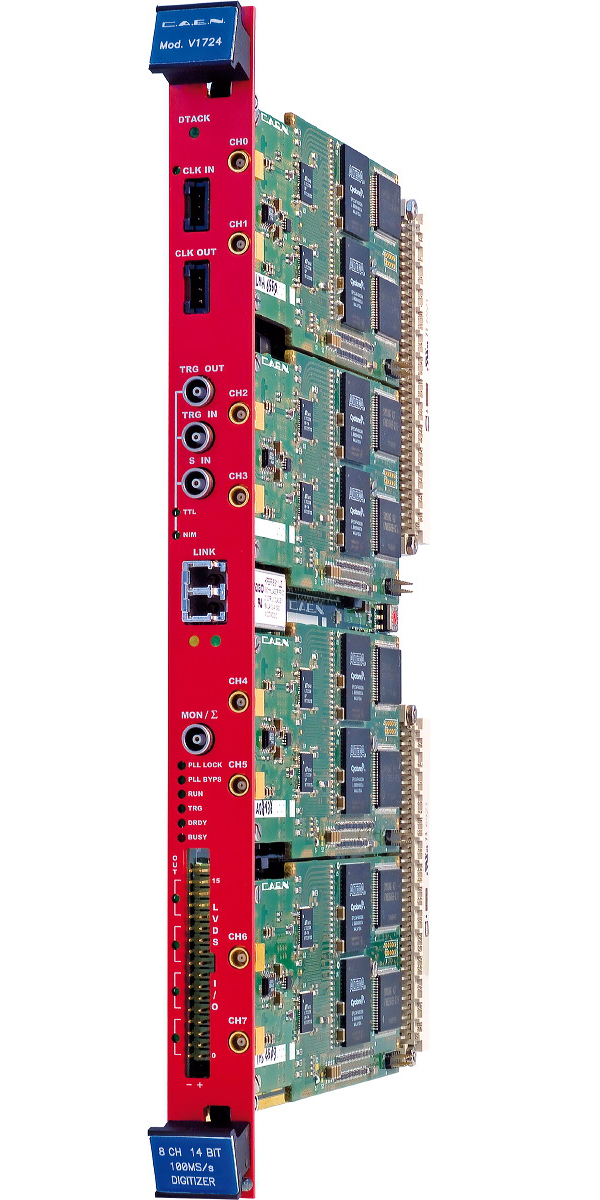
\includegraphics[height=3in]{images/V1724}\label{fig:CAENDIGI}}&
	\subfigure[V1718 Controller]{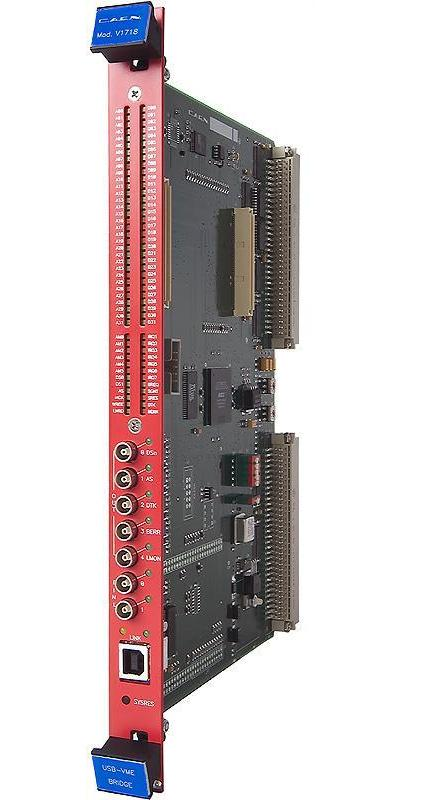
\includegraphics[height=3in]{images/Controller}\label{fig:CAENCON}} \\
    \end{tabular}
    \caption[CAEN VME modules used for DAQ]{CAEN VME modules used for DAQ.}% Specifications can be found in Table~\ref{tab:CAENSPEC}}
    \label{fig:VMEmod}
\end{figure}


	DAQ software was written to combine the CAEN digitizer libraries, the \textbf{E}xperimental \textbf{P}hysics and \textbf{I}ndustrial \textbf{C}ontrol \textbf{S}ystem (EPICS) \cite{EPICS}, and the ROOT data analysis framework \cite{CERNROOT}. EPICS is used for slow control of all BEAST~II subsystems and to get real time plots of the data as the experiment is running. In the case of the \he tubes, EPICS controls starting and stopping of acquisition and reports the rate of hits in the \he tubes to the operator. ROOT ntuples containing the channel number, pulse height, and time stamp (in seconds since January 1, 1970) are saved to disc by the DAQ software.


	The digitizer has a 21~s (30 bit counter, 20~ns/bit) clock on board which is used to set the time stamp. After 21~s, this internal clock resets to 0 which the CAEN software accounts for on the next trigger. Unfortunately, when the clock rolls over multiple times without a trigger, the CAEN software assumes the clock has only rolled over once, leading to an incorrect time stamp. To prevent this, EPICS sends a software trigger to the digitizer every 10~s to ensure that the clock never rolls over more than once between triggers. This 0.1~Hz software trigger rate is subtracted from the \he tube hit rate in the analysis.



\section{Calibration}

After Phase~I was complete, the \he tubes were shipped back to the University of Victoria for calibration. This was a calibration of the whole system: the tubes themselves, the preamplifiers, the digitizer, and GEANT4 (v10.3). During the calibrations, each tube was connected to the same channel that it was during Phase~I.

\subsection{Neutron Source}
\label{sec:AmBe}
	The University of Victoria has a 241-AmBe neutron source, which produces neutrons using the following reaction \cite{barschall1983neutron}:

\begin{subequations}
\begin{align}
		{^{241}_{95}\mathrm{Am}\rightarrow~^{237}_{93}\mathrm{Np} + ^4_2\mathrm{He} + \gamma}\\
		{^9_4\mathrm{Be}+^4_2\mathrm{He}\rightarrow~^{12}_6\mathrm{C}+^1_0\mathrm{n}+\gamma}
\end{align}
\end{subequations}
with an activity of 168~GBq (measured at 185~GBq in 1966). The energy spectrum of an AmBe source can be found in Fig~\ref{fig:AmBeSpec}. The configuration of the University of Victoria's AmBe source can be found in~\cite{hargrove}. The neutron rates from five different AmBe sources is measured in \cite{lebreton2007experimental}. From this, it is determined that an AmBe source produces 6.08$\pm$0.17$\times10^{4}$~neutrons/GBq. For the 168~GBq source, this corresponds to 1.02$\pm$0.03$\times10^{7}$~neutrons/s.

The source is surrounded by a cube of graphite 1.83~m to a side, which thermalizes the neutrons. The spectrum of the neutrons which emerge from the graphite is shown in Fig~\ref{fig:afterGraphite}. For reference, the efficiency of the \he tubes over a large kinetic energy range is shown in Fig~\ref{fig:he3eff}. Using data from these figures, the \he tubes are able to detect 62\% of the neutrons which emerge from the graphite cube. Graphite can contain boron impurities, but since the graphite used next to the source is `medium grade' it is assumed that there is no significant absorption of neutrons by boron impurities. This graphite has a density of (1.63$\pm$0.01)~g/cm$^3$~\cite{AmBELetter}. This source provides an excellent tool for testing and calibrating the \he tubes. 

\begin{figure}
	\centerfloat
		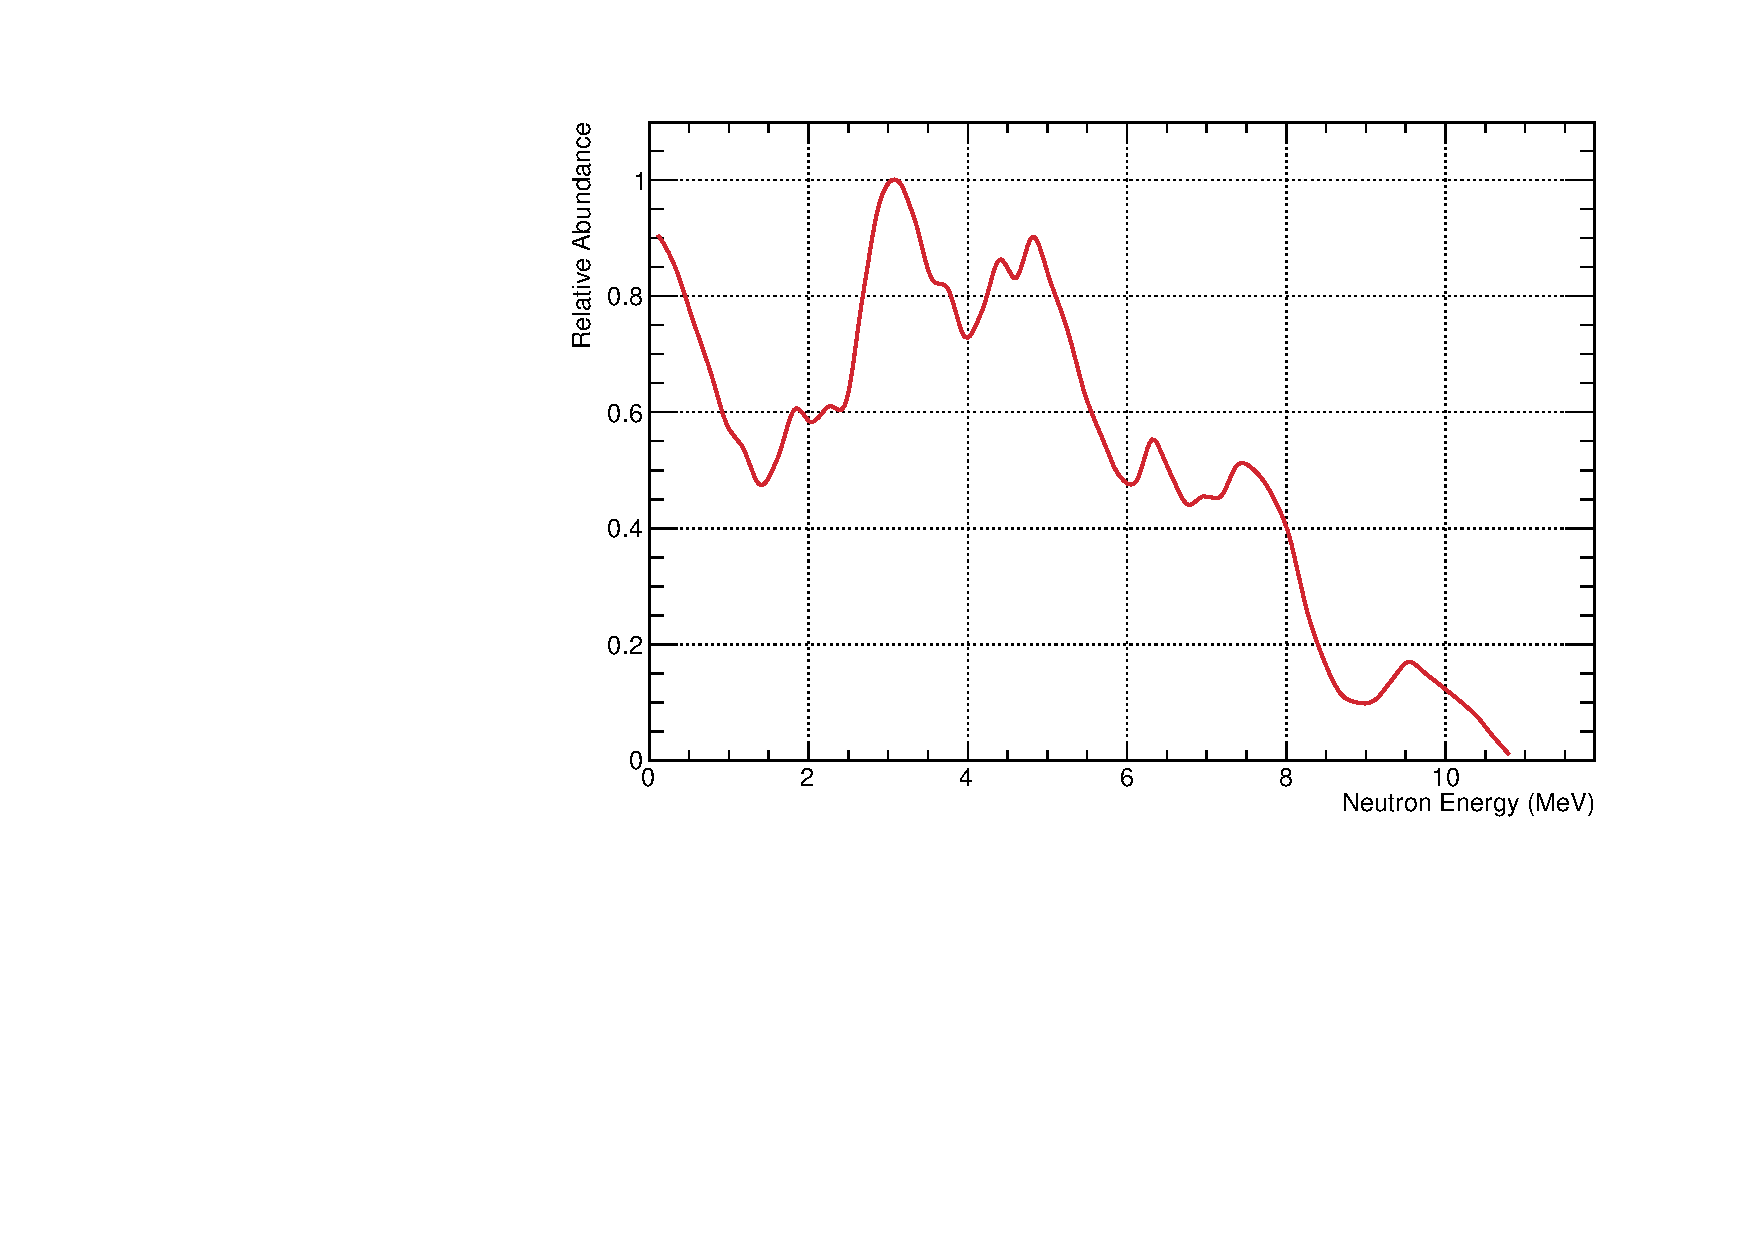
\includegraphics[trim={0 0 0 0.75cm},clip, width=\textwidth]{images/AmBe_NeutronSpectrum.pdf}
	\caption[Energy spectrum of neutrons from AmBe source]{Energy spectrum of neutrons from AmBe source~\cite{AmBeSpec}.}
	\label{fig:AmBeSpec}
\end{figure}


\begin{figure}
	\centerfloat
		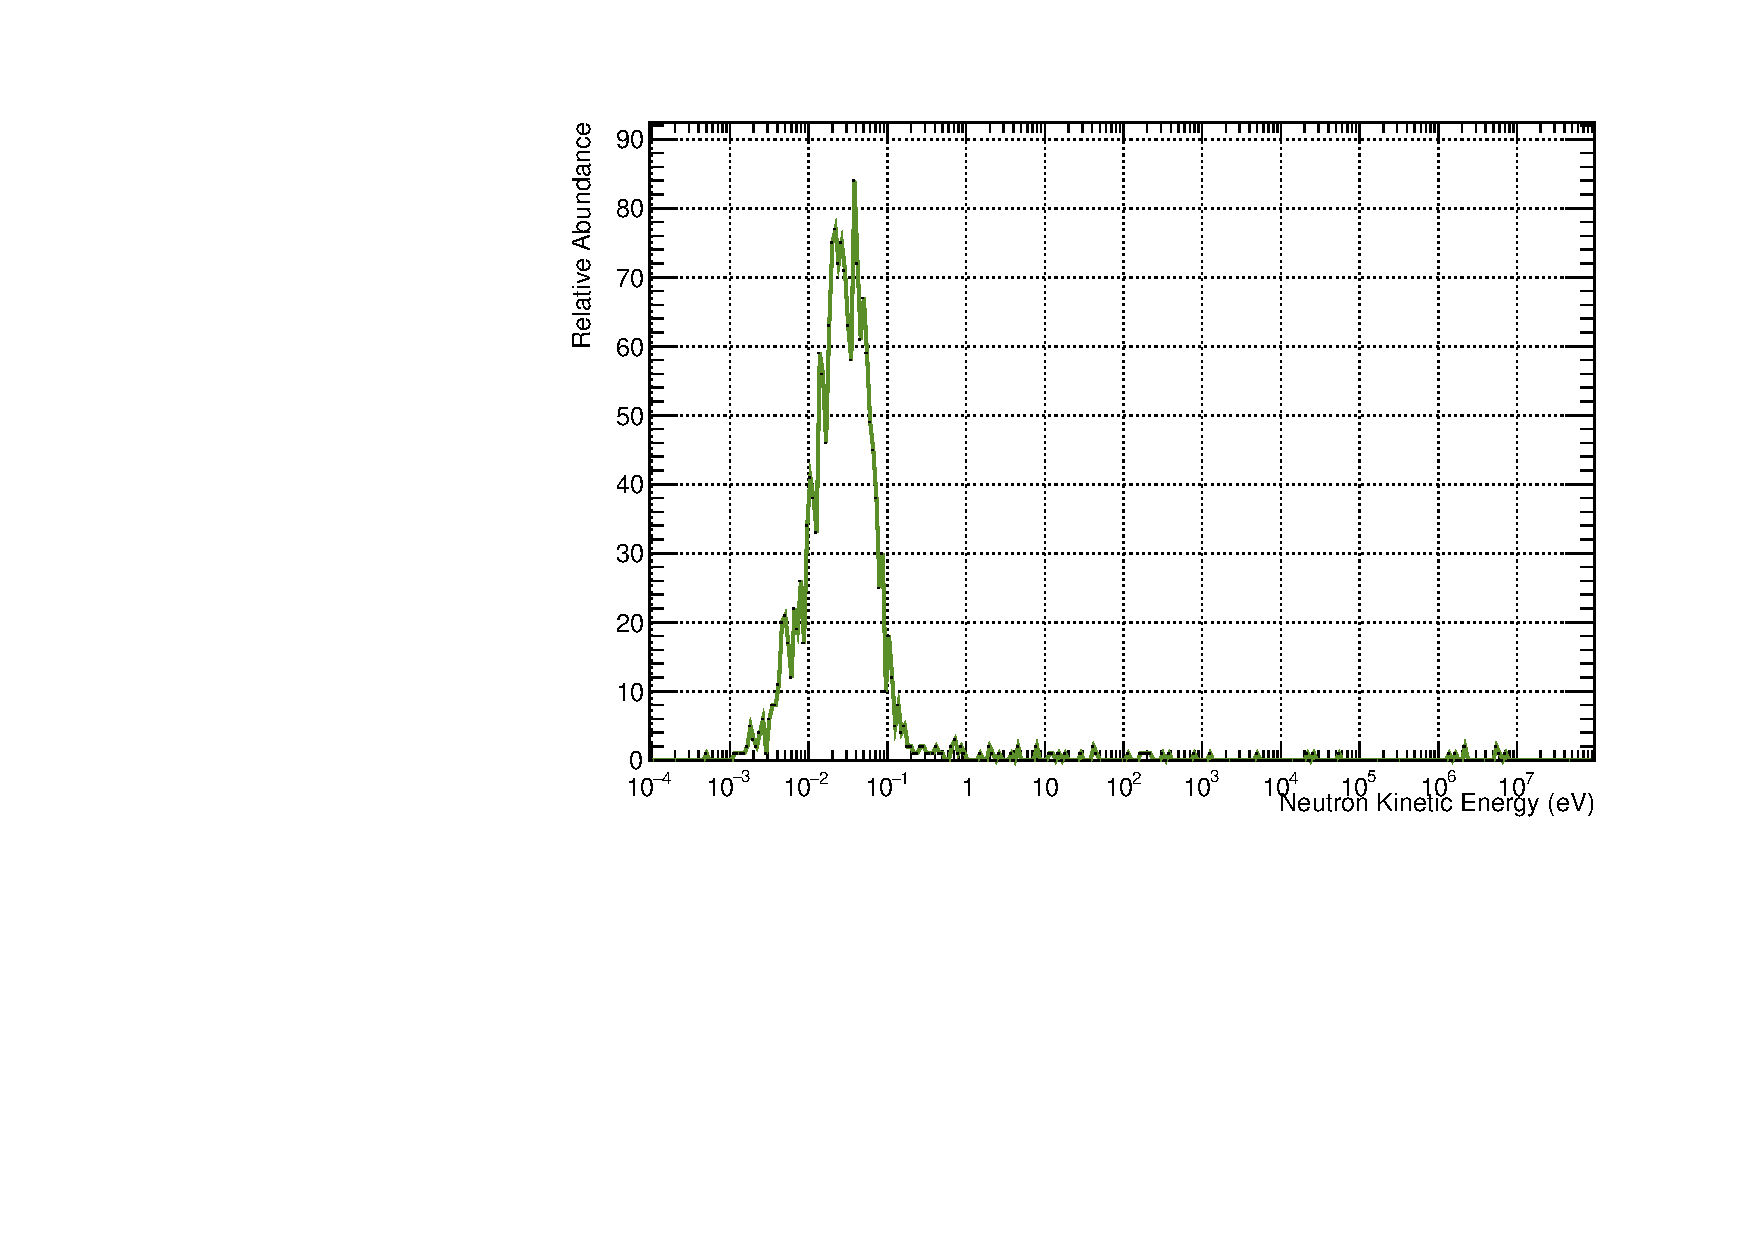
\includegraphics[trim={0 0 0 0.75cm},clip, width=\textwidth]{images/AfterGraphite}
	\caption[Kinetic energy spectrum of neutrons after they pass through the graphite cube]{Kinetic energy spectrum of neutrons after they pass through the graphite cube. From simulation in GEANT4.}	
	\label{fig:afterGraphite}
\end{figure}


\begin{figure}
	\centerfloat
		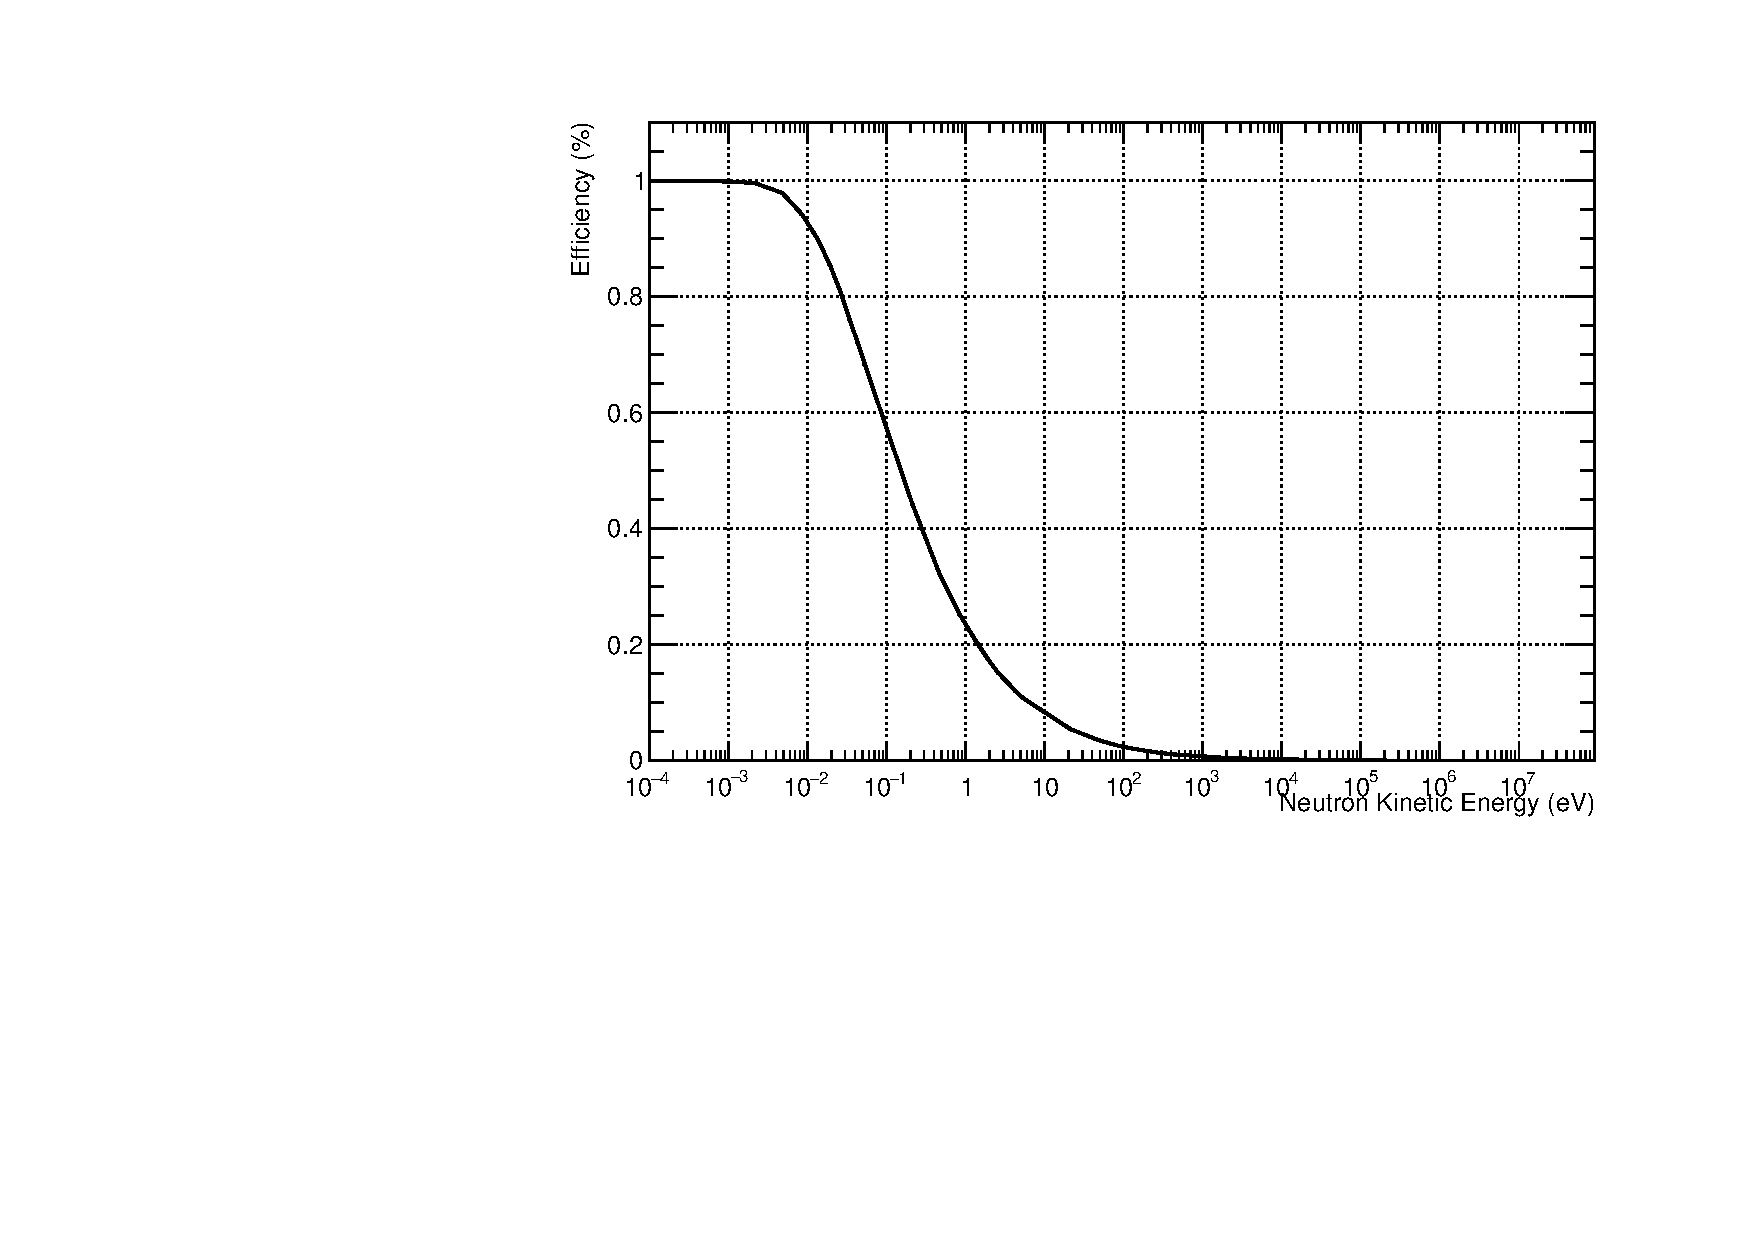
\includegraphics[trim={0 0 0 0.75cm},clip, width=\textwidth]{images/Efficiency_inside}
	\caption[Efficiency of \he tubes vs kinetic energy]{Efficiency of \he tubes vs kinetic energy, from simulation in GEANT4.}
	\label{fig:he3eff}
\end{figure}


\subsection{Calibration Procedure}


\subsubsection{Gain Matching}

	The \he tubes were returned to the University of Victoria after Phase~I of BEAST~II operation for calibration. During testing, it was observed that the pulse height spectrum for each \he tube did not match the pulse height spectrum from the same tube in Phase~I, despite having the HV supply set to the same voltage (see Fig~\ref{fig:pulseHeightSpectrumDifferenceBaA}). It is unclear what caused this issue, but subsequent measurements of the output voltage of the Bertran supply suggests that it was not as stable as expected. In order to get an accurate calibration, it was necessary to choose an HV setting that caused the pulse height spectrum to match what was observed in Phase~I. 

	The \he tubes were run at 2~V increments starting from 1540~V up to 1590~V. For each voltage setting, $\chi^2$ comparison was done between the spectrum observed in Phase~I and the spectrum observed at that voltage. The voltage that produced the lowest $\chi^2$ was used as the operating voltage for that tube during calibration. Table~\ref{tab:Tubevoltage} summarizes the voltage settings used in Phase~I. 


\begin{figure}
	\centering
	\subfigure[Channel 0]{
		\begin{overpic}[trim={0 0 0 0.5cm},clip, width=0.47\textwidth]{images/VoltageTestChannel0.pdf}
		\end{overpic}
		\label{fig:VoltageChannel0}
	}
	\subfigure[Channel 1]{
		\begin{overpic}[trim={0 0 0 0.5cm},clip, width=0.47\textwidth]{images/VoltageTestChannel1.pdf}
		\end{overpic}
		\label{fig:VoltageChannel1}
	}
	\subfigure[Channel 2]{
		\begin{overpic}[trim={0 0 0 0.5cm},clip, width=0.47\textwidth]{images/VoltageTestChannel2.pdf}
		\end{overpic}
		\label{fig:VoltageChannel2}
	}
	\subfigure[Channel 3]{
		\begin{overpic}[trim={0 0 0 0.5cm},clip, width=0.47\textwidth]{images/VoltageTestChannel3.pdf}
		\end{overpic}
		\label{fig:VoltageChannel3}
	}
	\caption[Pulse height spectra before and after voltage correction]{Pulse height spectra of thermal neutrons before and after voltage correction. Red is during Phase~I, blue is at 1580 V, and green is at the corrected voltage.}
	\label{fig:pulseHeightSpectrumDifferenceBaA}
\end{figure}




\paragraph{Uncertainty on the rate due to the voltage setting} Since the voltage that was used to calibrate the \he tubes is not exactly the same as the voltage used in Phase~I, there is an uncertainty in the calibrated rate. To quantify this uncertainty, the rate at the chosen voltage setting was compared to the rates measured at +2~V and -2~V, since these were the smallest voltage increments studied and serve as a conservative uncertainty. The uncertainty due to the voltage setting is then:
\begin{equation}
	{\sigma_{\pm} = |R_{\mathrm{nominal}} - R_{\mathrm{nominal}\pm2\mathrm{ V}}| }
\end{equation}
The values of $\sigma_{\pm}$ are presented in Table~\ref{tab:VoltageUncertainty}.





\begin{table}[htb]
	\centering
	\begin{tabular}{ cc }
	Channel	& Voltage (V)	\\ \hline \hline
	0	& 1586	\\
	1	& 1570	\\
	2	& 1550	\\
	3	& 1560	\\ \hline
	\end{tabular}
	\caption[Nominal high voltage settings during \he tube calibration]{Nominal high voltage settings during \he tube calibration.}
	\label{tab:Tubevoltage}
\end{table}


\begin{table}[htb]
	\centering
	\begin{tabular}{ cccccc }
	&	\multicolumn{3}{c}{Rate at} & & \\
Channel	&	-2~V (Hz)	&	Nominal (Hz)	&	+2~V (Hz)	&	$\sigma_+$ (Hz)	&	$\sigma_{-}$ (Hz)	\\ \hline
0	&	199.0	&	191.6	&	184.8	&	7.47	&	6.75	\\
1	&	218.4	&	214.2	&	198.0	&	4.20	&	16.24	\\
2	&	140.3	&	146.2	&	158.5	&	12.35	&	5.93	\\
3	&	255.8	&	262.1	&	271.8	&	6.38	&	9.64	\\ \hline
	\end{tabular}
	\caption[Uncertainty on \he tube rate due to voltage uncertainty]{Uncertainty on \he tube rate due to voltage uncertainty.}
	\label{tab:VoltageUncertainty}
\end{table}





\subsection{Calibration}

To calibrate the \he tubes, each tube was placed one at a time into a cradle made of high density polyethylene (HDPE). The polyethylene reduced the thermal neutron flux in the source room from $\sim$600~Hz to $\sim$100~Hz, similar to that observed in Phase~I of BEAST~II, by absorbing some of the thermal neutrons. The relative orientation of the \he tubes and the graphite is shown in Fig~\ref{fig:he3CalibPosn}. 

\begin{figure}[htb]
	\centerfloat
	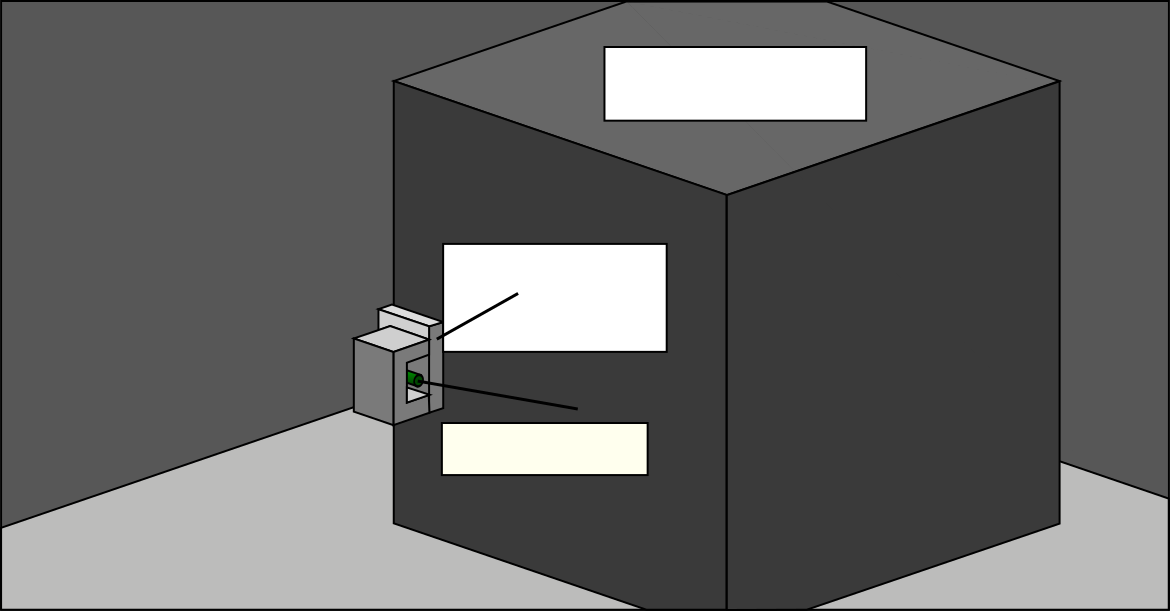
\includegraphics[height=8cm]{images/GEANTVis2}
	\caption[\He tube calibration setup]{\He tube calibration setup from GEANT4 simulation, including HDPE cradle. Image is to scale.}	
	\label{fig:he3CalibPosn}
\end{figure}



The rate in each \he tube was recorded, then the cradle was moved to a position further from the source and the process was repeated. The rate in each \he tube as a function of the distance from the source is given in Fig~\ref{fig:he3rateVsD}.



\subsubsection{AmBe Source Simulation}
\label{sec:ambesim}

	A simulation of the AmBe source was produced using GEANT4 \cite{GEANT}. The simulation contains the source, the graphite cube (using the GEANT4 default density of 1.7~g/cm$^3$ instead of 1.63~g/cm$^3$), the concrete walls of the room, the HDPE cradle, and the \he tube. Neutrons following the spectrum shown in Fig~\ref{fig:AmBeSpec} are fired isotropically from the centre of the graphite cube. 1.0$\times10^{7}$ events corresponds to 1 second.


\begin{figure}
	\centerfloat
		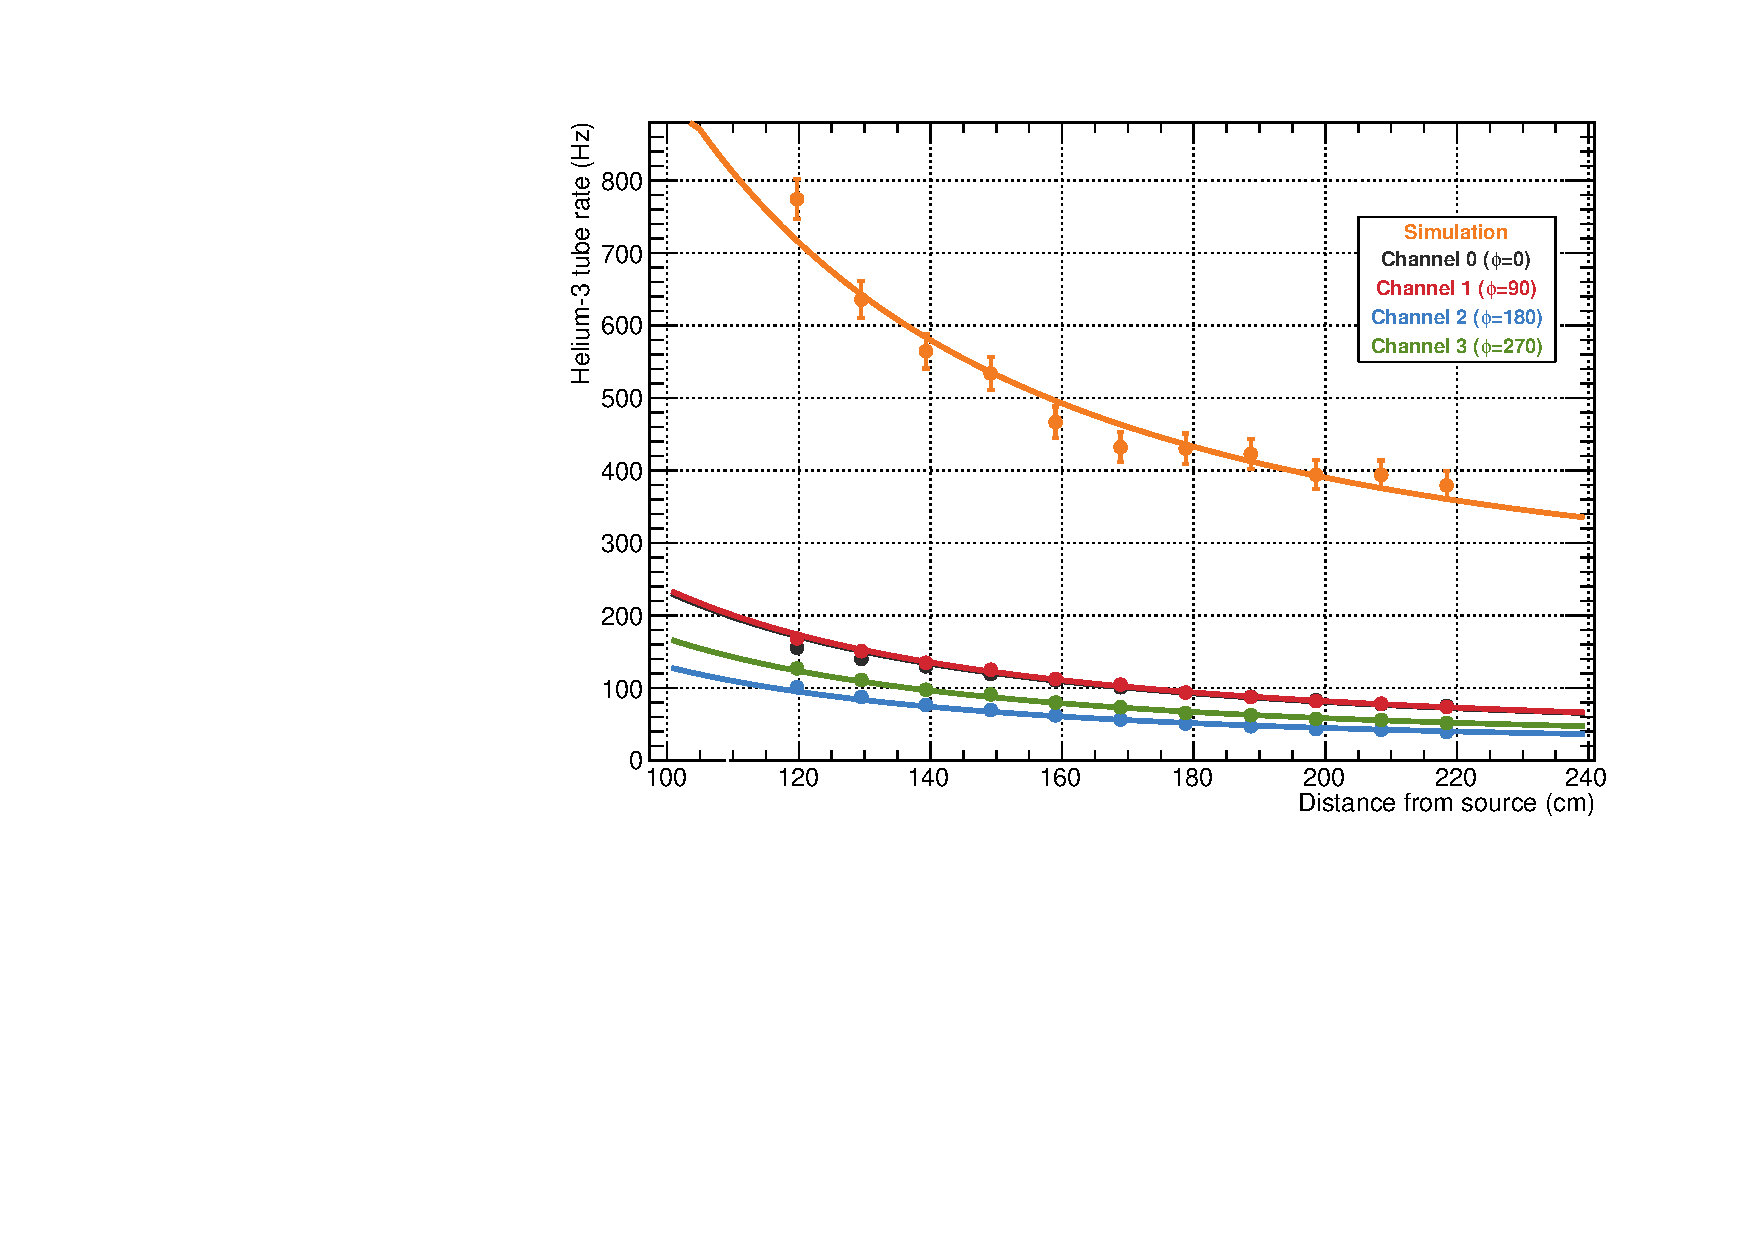
\includegraphics[trim={0 0 0 0.75cm},clip, width=\textwidth]{images/Parallel_Calibration}
	\caption[\He tube rate vs distance from thermal neutron source]{\He tube rate vs distance from thermal neutron source. Orange is simulation, other colours are the different channels. The measured minus fit rates are presented in Fig~\ref{fig:he3rateVsDUncertainty}.}	
	\label{fig:he3rateVsD}
\end{figure}

\begin{figure}
	\centerfloat
		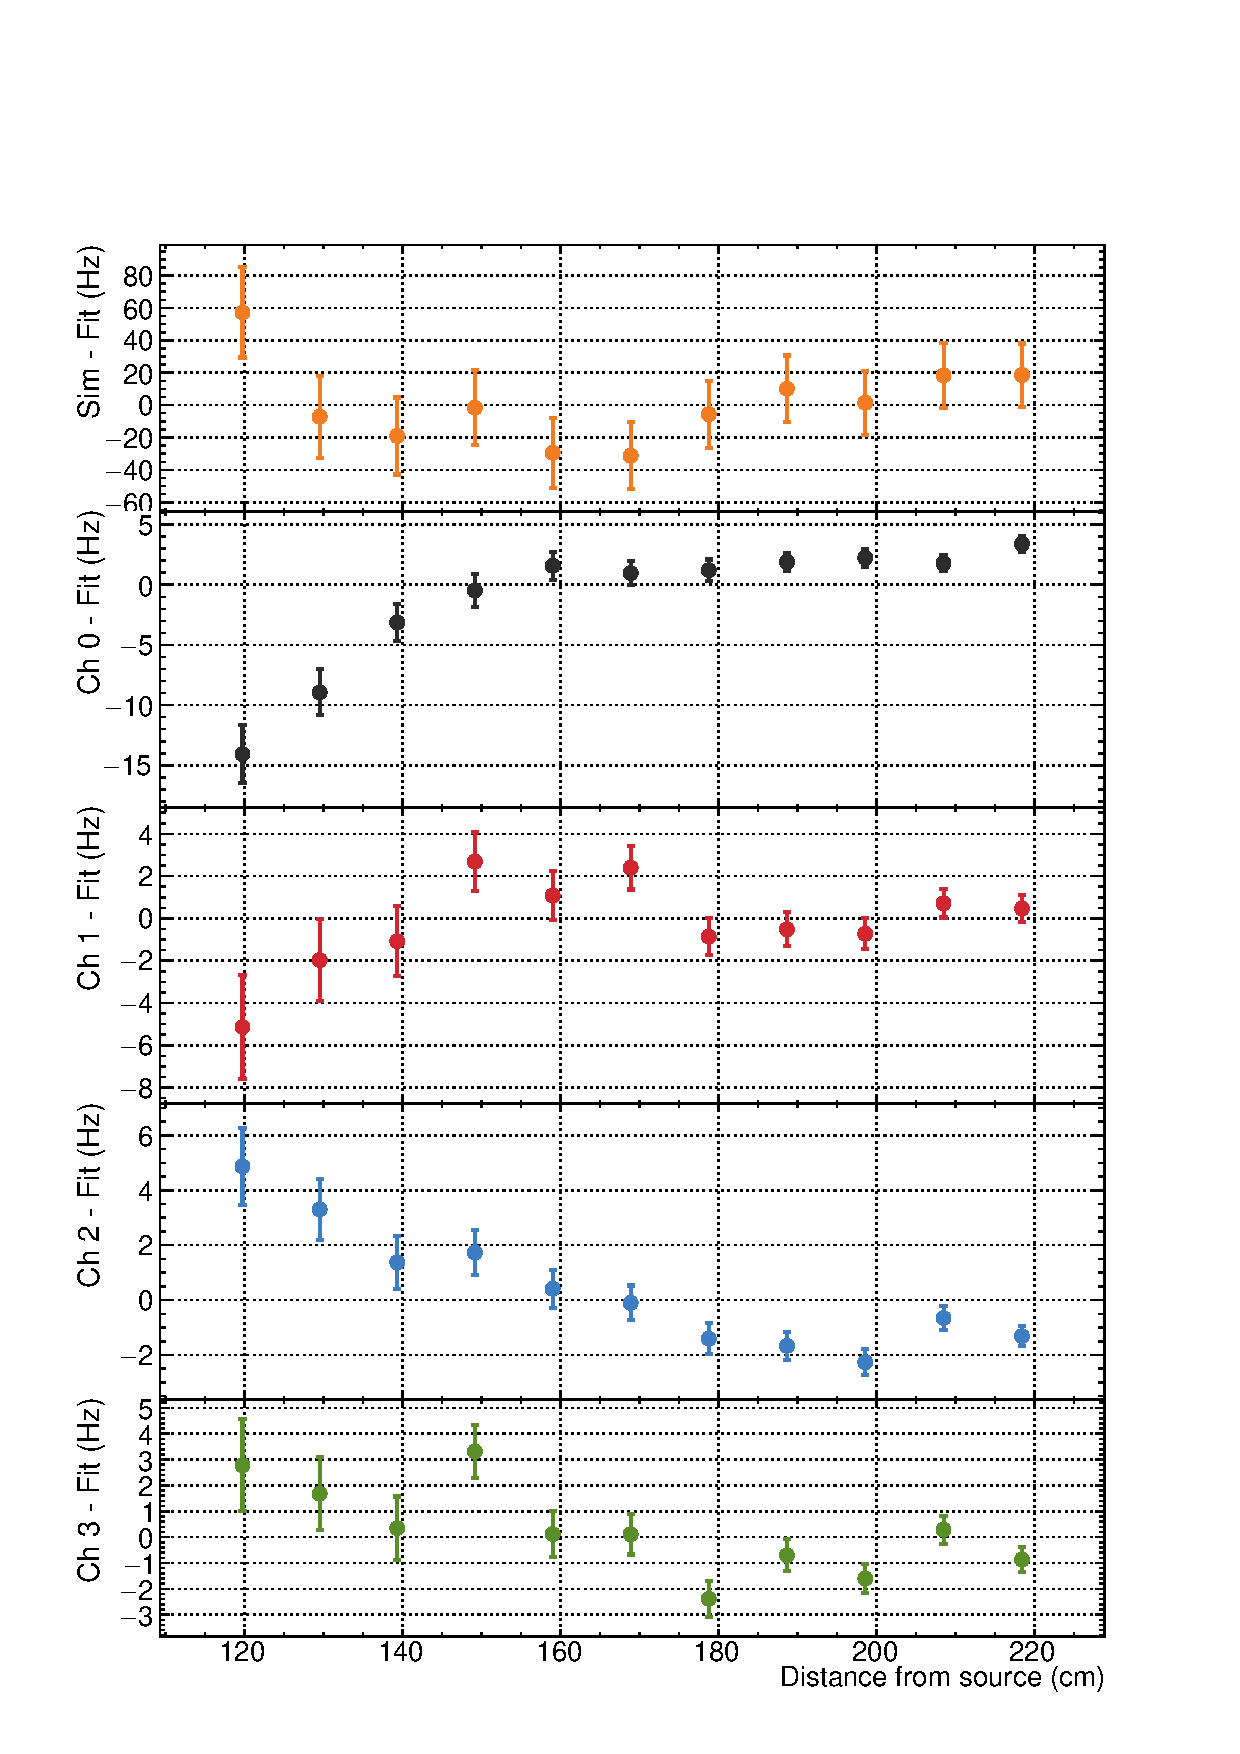
\includegraphics[width=\textwidth]{images/Parallel_Calib_Uncertainties}
	\caption[\He tube rate minus fit vs distance from thermal neutron source]{\He tube rate minus fit vs distance from thermal neutron source. Orange is simulation, other colours are the different channels. The errors are statistical only.}	
	\label{fig:he3rateVsDUncertainty}
\end{figure}


\subsubsection{Curve Fitting}

	The rates are fit to an inverse square function:
\begin{equation}
	{R_{n} = A_{n}\times\left(\frac{B}{(r-r_{0})^2}+C\right)}
	\label{eqn:invSq}
\end{equation}	
where $r$ is the position of the \he tube relative to the AmBe source. The parameters $B$, $C$, and $r_{0}$ are shared by the four \he tubes, while $A_{n}$ varies in each \he tube.

The AmBe source room is significantly more complex than just a graphite cube with a source at its centre as there is a large amount of equipment and storage in the room. This extra material is very difficult to simulate, but should manifest as a background neutron rate in the room, and thus only affect the `C' term in the fit. Therefore, a modified version of Eqn~\ref{eqn:invSq} is used for the simulation:
\begin{equation}
	{R_{\mathrm{sim}} = A_{\mathrm{sim}}\times\left(\frac{B}{(r-r_{0})^2} + C\right)+C_{\mathrm{sim}}}
\end{equation}	
The parameters $B$, $C$, and $r_0$ are the same as used in the fit to data. The fit to data and simulation are done simultaneously, with $A_{\mathrm{sim}}$ fixed at 1. $A_{n}$ is therefore the efficiency of each tube relative to the simulation. The efficiency for each \he tube is presented in Table~\ref{tab:he3Calib}.  The other fit parameters can be found in Table~\ref{tab:CalibrationFitPars}. The uncertainty due to the voltage setting is calculated as:
\begin{equation}
	{\sigma_{\pm}^V = A_{n}\frac{\sigma_{\pm}}{R}}
\end{equation}
where $\sigma_{\pm}$ and $R$ are taken from Table~\ref{tab:VoltageUncertainty}. 

Additionally, a 3\% uncertainty is added to account for the uncertainty on the number of neutrons produced by the AmBe source (see \S~\ref{sec:AmBe}).

The uncertainties due to the voltage, the neutron production rate, and from the fit are combined in quadrature to get the total uncertainty.

The measured rate minus the fit rate is shown in Fig~\ref{fig:he3rateVsDUncertainty}.

\begin{table}[htb]
	\centering
	\begin{tabular}{ cccccccccc}
Channel	&	$A_{n}$	&	$\sigma^{\mathrm{fit}}$	&	$\sigma_{+}^{V}$	&	$\sigma_{-}^{V}$	&	$\sigma^{\mathrm{AmBe}}$&		$\sigma_{+}^{\mathrm{Tot}}$	&	$\sigma_{-}^{\mathrm{Tot}}$	\\	\hline	\hline
0	&	0.278	&	0.019	&	0.011	&	0.010	&	0.008	&	0.023	&	0.021	\\		
1	&	0.282	&	0.020	&	0.006	&	0.021	&	0.008	&	0.021	&	0.029	\\		
2	&	0.154	&	0.011	&	0.013	&	0.006	&	0.005	&	0.017	&	0.013	\\		
3	&	0.201	&	0.014	&	0.007	&	0.005	&	0.006	&	0.016	&	0.015	\\	\hline	
	


	\end{tabular}
	\caption[\He tube efficiency with uncertainties]{\He tube efficiency with uncertainties. $\sigma^{\mathrm{fit}}$ is the uncertainty from the fitting, $\sigma_{\pm}^{V}$ is the uncertainty from the voltage, and $\sigma^{\mathrm{AmBe}}$ is the uncertainty from the neutron production rate.}
	\label{tab:he3Calib}
\end{table}

\begin{table}[htb]
	\centering
	\begin{tabular}{ lrrr }
Parameter		& Value		& Uncertainty	 \\ \hline \hline
	$\chi^2$		& 215.361	& 		\\
	degrees of freedom		& 47		&		\\
	$B\times10^{6}$ cm$^2$s$^{-1}$ 	&	7.243 	& 0.822 	\\	
$	r_{0}$ (cm)	&	0 			& 4.6 	\\	
	$C$ (Hz)	&	107.856				& 10.2 	\\	
$	A_{0}	$	&	0.278				& 0.019	\\	
$	A_{1}	$	&	0.282				& 0.020	\\	
$	A_{2}	$	&	0.154				& 0.011	\\	
$	A_{3}	$	&	0.201				& 0.014	\\	
$	A_{\mathrm{sim}}	$	&	1.000				& N/A	\\	
$	C_{\mathrm{sim}}	$ (Hz)	&	100.455				& 26.4 	\\	\hline

	\end{tabular}
	\caption[Fit parameters for calibration fit shown in Fig~\ref{fig:he3rateVsD}]{Fit parameters for calibration fit shown in Fig~\ref{fig:he3rateVsD}.}
	\label{tab:CalibrationFitPars}
\end{table}

\paragraph{Uncertainty on points}

	The uncertainty on the simulated points is the square root of the number of simulated hits divided by number of seconds that have been simulated:
\begin{equation}
	\sigma_{\mathrm{rate}} = \frac{\sqrt{N_{\mathrm{events}}}}{t}
	\label{eqn:rateUncertainty}
\end{equation}

	The measured data have two associated uncertainties: the uncertainty on the rate, and the uncertainty on the position. The uncertainty on the rate is the same as also given by Eqn~\ref{eqn:rateUncertainty}. The uncertainty on the position is taken to be 1 cm. 

The position uncertainty is converted to a rate uncertainty using standard propagation of error:
\begin{equation}
	\sigma_{\mathrm{rate}}^{\mathrm{position}} = \frac{\partial R_{n}}{\partial r}\sigma_{r}= 2\frac{A_{n}B}{(r-r_0)^3}\sigma_{r}
	\label{eqn:posUncert}
\end{equation}
where $R_{n}$ is given by Eqn~\ref{eqn:invSq}.
Equations~\ref{eqn:rateUncertainty} and~\ref{eqn:posUncert} are added in quadrature to get the total rate uncertainty. Since the uncertainty due to the position requires fit parameters to calculate, the fit is first calculated, then the uncertainty on the rate due to position is calculated. The fit is then recalculated until the fit parameters converge. The uncertainty on the rate is shown in Fig~\ref{fig:he3rateVsDUncertainty}.

\paragraph{Discussion of $\chi^{2}$}

	As evident from Table~\ref{tab:CalibrationFitPars}, the $\chi^2$ of the calibration fit is quite high. Because the fit is done for all four tubes and simulation simultaneously, an outlying point in one of the tubes affects the whole calibration. In Fig~\ref{fig:he3rateVsD}, the first three points of channel 0 are outliers. These are the main contribution to the large $\chi^2$ value. If these first three points are removed and the fit is recalculated, $\chi^2$ becomes 110.4, with 44 degrees of freedom. A comparison of the efficiencies ($A_{n}$) and C$_{\mathrm{sim}}$ with and without these points can be found in Table~\ref{tab:he3ChiCompare}. The values of $A_{n}$ are consistent within 1 $\sigma$.

\begin{table}[htb]
	\centering
	\begin{tabular}{ccccc}
	&		&		&	 \multicolumn{2}{c}{Removing first three}			\\	
	&	 \multicolumn{2}{c}{All points}			&	 \multicolumn{2}{c}{points of channel 0}			\\	
Channel	&	$A_{n}$	&	$\sigma_{A_{n}}$	&	$A_{n}$	&	$\sigma_{A_{n}}$	\\ \hline \hline	
0	&	0.278	&	0.019	&	0.294	&	0.020	\\	
1	&	0.282	&	0.020	&	0.294	&	0.020	\\	
2	&	0.154	&	0.011	&	0.160	&	0.011	\\	
3	&	0.200	&	0.014	&	0.209	&	0.014	\\	
C$_{\mathrm{sim}}$ &  100.455 & 26.4    &	114.324 &	25.186  \\	\hline

	\end{tabular}
	\caption[\He tube efficiencies with and without first three channel 0 points]{\He tube efficiencies with and without first three channel 0 points.}
	\label{tab:he3ChiCompare}
\end{table}


\paragraph{Cross Check on \He Tube Efficiency}

	The uncertainty on the \he tube efficiency is the uncertainty on the fitting parameters shown in Table~\ref{tab:CalibrationFitPars}. As a cross check, a simple analysis was done.

	Each simulated point has the parameter $C_{\mathrm{sim}}$ subtracted from it. Then, for each data point, an estimate of $A$ was calculated:
\begin{equation}
	A_{\mathrm{Estimate}} = \frac{R_{\mathrm{real}}}{R_{\mathrm{sim}}-C_{\mathrm{sim}}}
\end{equation}
For each tube, the mean and RMS of this was calculated for all points in Fig~\ref{fig:he3rateVsD} (Table~\ref{tab:CrossCheck}). The RMS calculated in this cross check was very similar to the fit uncertainties shown in Table~\ref{tab:CalibrationFitPars}, which provides evidence that the fitting uncertainties are appropriate, even for large $\chi^2$.


\begin{table}[htb]
	\centering
	\begin{tabular}{ ccc }
Channel	&	$A_{\mathrm{Estimate}}$	&	RMS	\\ \hline \hline	
0	&	0.275	&	0.020	\\	
1	&	0.281	&	0.019	\\	
2	&	0.155	&	0.011	\\	
3	&	0.201	&	0.012	\\	\hline

	\end{tabular}
	\caption[Cross check of uncertainty on \he tube efficiency]{Cross check of uncertainty on \he tube efficiency.}
	\label{tab:CrossCheck}
\end{table}





	%To quantify the uncertainty on the \he tube efficiency, the maximum and minimum value of this equation was used:

%	Each simulated point had the parameter $C_{sim}$ subtracted from it. Then for each tube, the maximum and minimum of $R_{real}/R_{sim}$ are found. The uncertainty $\sigma_{\pm}^{fit}$ is then defined as:
%\begin{equation}
%\sigma_{\pm}^{fit} = |A_{n} - A_{n}^{\pm}|
%\end{equation}
%where $A_{n}^{+}$ is the maximum value of $R_{real}/R_{sim}$, and $A_{n}^{-}$ is the minimum.  The uncertainty from the fitting was combined with the uncertainty due to the voltage to get the total uncertainty. The uncertainties can be found in Table~\ref{tab:he3Calib}



%	To quantify the uncertainty on the \he tube efficiency, the fitting of the \he tube vs distance from the source was repeated, ignoring the first four data points, as these have the largest deviation from the fit shown in~\ref{fig:he3rateVsD}. The fit was then repeated ignoring the last six data points. The efficiencies produced by these fits provided an upper and lower bound on the values for the \he tube efficiency, and are used as uncertainty on the fit. Plots of these fits can be found in Appendix~\ref{chap:calibUn}. The uncertainty from the fitting was combined with the uncertainty due to the voltage to get the total uncertainty. The uncertainties can be found in Table~\ref{tab:he3Calib}.
	

	%The fit shown in Fig~\ref{fig:he3rateVsD} 


\section{Deployment in BEAST~II Phase~I}



\begin{figure}[htb]
	\centerfloat
		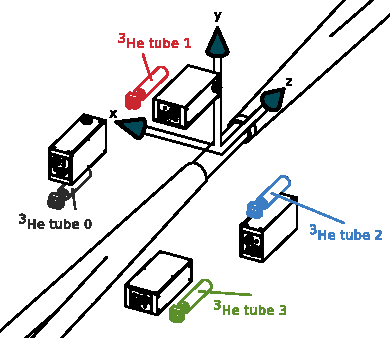
\includegraphics[width=\textwidth]{images/he3tubesAndTPCs}		
	\caption[\He tube and TPCs in BEAST~II Phase~I]{\He tube and TPCs in BEAST~II Phase~I. Colour scheme is the same as used in various plots, such as Fig~\ref{fig:he3rateVsD}. The centre of the SuperKEKB rings is in the negative $x$ direction.}
    \label{fig:He3InSitu}
\end{figure}

In Phase~I of BEAST~II, the \he tubes were placed at the locations above, below, and on either side of the IR as shown in Table~\ref{tab:he3Loc}. They were mounted beside the TPC positions (see \S~\ref{sec:TPCs}), as shown in Fig~\ref{fig:He3InSitu}.



\begin{table}[htb]
	\centering
	\begin{tabular}{ rrrrr }
	Channel	&	x (m)	&	y (m)	&	z (m)	&	$\phi$ (approximate)	\\ \hline \hline
	0	&	0.439	&	0.073	&	0.469	&	0$^{\circ}$	\\
	1	&	-0.130	&	0.469	&	0.517	&	90$^{\circ}$	\\
	2	&	-0.477	&	-0.083	&	0.485	&	180$^{\circ}$	\\
	3	&	0.052	&	-0.451	&	0.470	&	270$^{\circ}$	\\ \hline
	\end{tabular}
	\caption[Locations of \he tubes]{Locations of \he tubes. IP is at (0,0,0), z runs parallel to the beampipe and the centre of the rings is in the negative $x$ direction.}
	\label{tab:he3Loc}
\end{table}



\section{Deployment in BEAST~II Phase~II}


\subsection{Magnetic Field Testing}

	In Phase~II of BEAST~II, most of the components of Belle~II will be in place and the magnetic field will be turned on. It was thus necessary to determine whether or not the \he tubes would be affected by the magnetic field, or if they would distort the field in an undesirable way. To test this, a single horseshoe magnet was placed with its poles pointing upward. A gaussmeter probe, supported by a lab stand, was placed between the poles. A \he tube, also supported by a lab stand, was placed in various locations near the probe, as shown in Fig~\ref{fig:apparatusSchematic}.

\begin{figure}[htb]
	\centering
	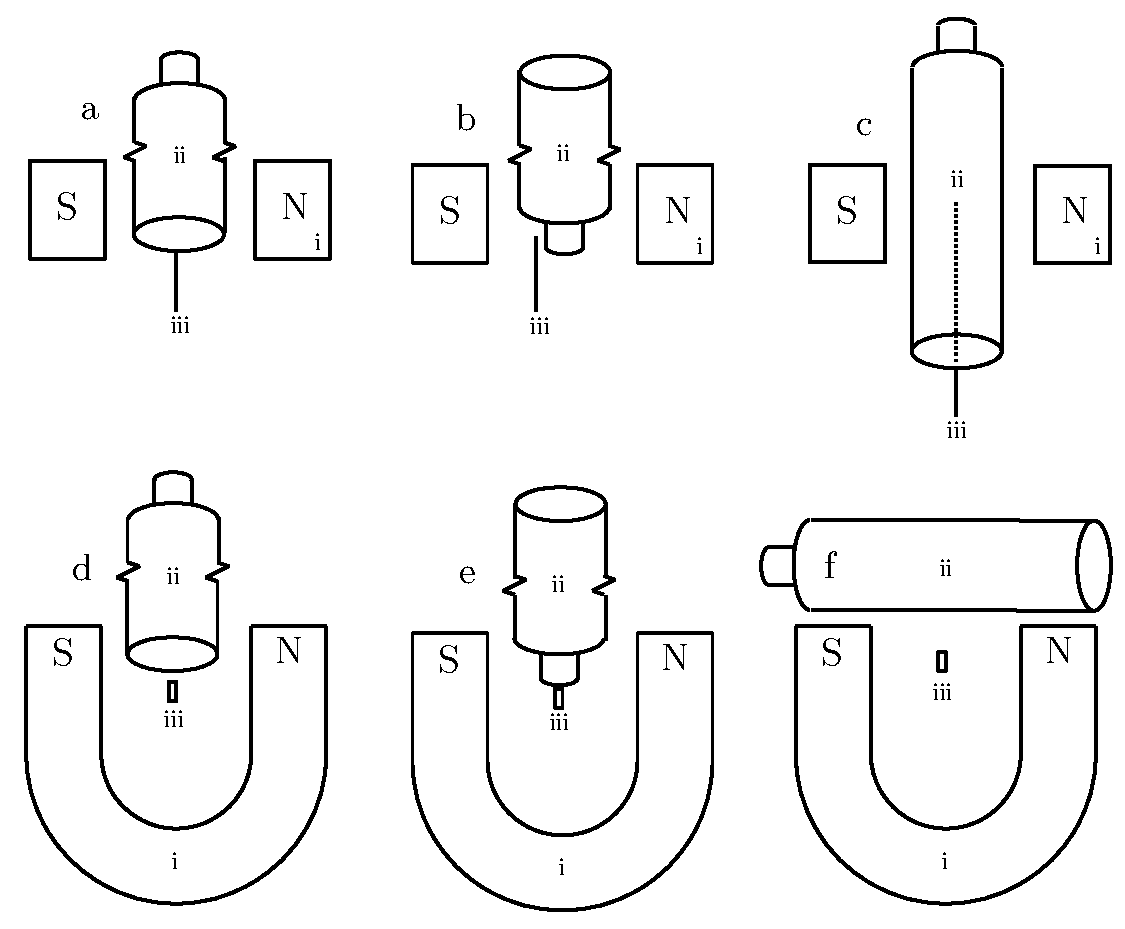
\includegraphics[width=\textwidth]{images/Apparatus_III}
	\caption[Schematic of \he tube and gaussmeter probe placement]{Schematic of \he tube and gaussmeter probe placement (not to scale). i is the magnet, ii is the \he tube, and iii is the gaussmeter probe.}	
	\label{fig:apparatusSchematic}
\end{figure}

The results of the experiment show that the detectors are non-magnetic (see Table~\ref{tab:magField}), and will therefore not shift in Belle~II's magnetic field, or disrupt the field around them.

\begin{table}[htb]
	\centering
	\begin{tabular}{ ccc }
		 & Field without \he  & Field with \he  	\\
		Position  &   tube present (kG)	  &  tube present (kG)      \\ \hline \hline
		a & 1.322 & 1.321 \\			
		b & 1.321 & 1.319 \\			
		c & 1.322 & 1.322 \\			
		d & 1.323 & 1.321 \\				
		e & 1.323 & 1.314 \\		
		f & 1.489 & 1.489 \\		\hline	
	\end{tabular}
	\caption[Results of magnetic field test]{Results of magnetic field test. Positions are described in Fig~\ref{fig:apparatusSchematic}.}
	\label{tab:magField}
\end{table}





\chapter{Beam Backgrounds}
\label{chap:beamBack}

	As electrons and positrons circle the HER and LER, some of them are lost from the beam as they collide with the residual gas in the beampipe and with other beam particles. These collisions move the particles out of a stable orbit, causing them to collide with the beampipe and other nearby materials, causing showers of particles. This chapter discusses some of the ways that particles can be lost from the beam and some of the effects of that loss.


\section{Beam-Gas Interactions}
\label{sec:beamGas}

\begin{figure}[htb]
	\centerfloat
		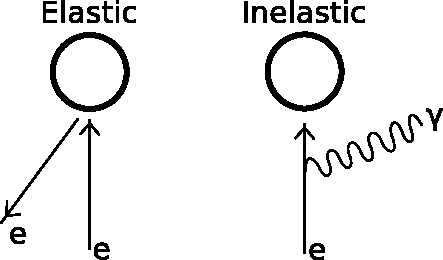
\includegraphics{images/beambeamCartoon}
	\caption[Beam-gas scattering]{Beam-gas scattering.}		
	\label{fig:BGasScat}
\end{figure}


\subsection{Elastic collisions}

	The beampipe is designed to operate under a vacuum of 10~nTorr and as such there are still residual gas atoms in the beampipe. When a beam particle collides with an atom of residual gas in the beampipe, the collision is elastic and there is very little kinetic energy transferred to the gas atom. The beam particle, however, undergoes a large scattering, which can send it outside the acceptance of the beam orbit. The cross section for this interaction is given by \cite{moller1999beam, Marin:1999ss}:
\begin{equation}
	{\sigma_{\mathrm{scatt}}=\frac{2\pi r_eZ^2}{\gamma^2}\frac{\beta_1\beta_2}{d^2}}
	\label{eqn:coulomb}
\end{equation}
where $r_{e}$ is the classical electron radius, $\gamma$ is the relativistic Lorentz factor, $Z$ is the atomic number of the target nucleus, $\beta_1$ and $\beta_2$ are the betatron functions, and $d$ is the size of beam aperture.


\subsection{Inelastic collisions}
\label{sec:brem}

	Beam particles emit bremsstrahlung radiation as they interact with the residual gas atoms in the beampipe. If the energy lost to the bremsstrahlung photon is high, the particle that emitted it will fall out of the momentum acceptance of the ring. The cross section for bremsstrahlung of electrons on atomic nuclei is given by \cite{moller1999beam, Marin:1999ss}:
\begin{equation}
	{\sigma_{\mathrm{brems}}=\frac{16r_e^2Z^2}{411}\ln\left [ \frac{183}{Z^{1/3}} \right ]\ln\left [ \frac{E}{\varepsilon _{RF}}-\frac{5}{8} \right ]}
	\label{eqn:brems}
\end{equation} 
where $r_e$ is the classical electron radius, $Z$ is the atomic number of the target nucleus, $\varepsilon _{RF}$ is the energy acceptance, and $E$ is the beam energy.

\subsection{Beam-Gas Beam Loss}

	The beam loss due to beam-gas effects is given by \cite{moller1999beam, malyshev2012gas}:
\begin{equation}
	{-\frac{1}{I}\frac{dI}{dt}=\frac{1}{\tau_{\mathrm{gas}}} = v\sum \sigma_{i} n_{i}}
\end{equation}
where $\tau_{\mathrm{gas}}$ is the beam lifetime from the beam-gas effects, $I$ is the beam current, $v$ is the velocity of the beam particles, $\sigma_{i}$ is the beam-gas cross section for each gas species, and $n_i$ is the atomic density of each species. If the gas mixture is constant, this can be rearranged to:
\begin{equation}
	{\frac{dI}{dt}\propto - I P}
	\label{eqn:simpleBeamGas}
\end{equation}
where $P$ is the beampipe pressure, which is proportional to the density of the gas.

If the gas mixture is changing, this change must be accounted for. Both the elastic and inelastic cross sections depend on $Z^2$. This modifies Eqn \ref{eqn:simpleBeamGas} to be:
\begin{equation}
	{\frac{dI}{dt}\propto  - I P Z^{2}}
	\label{eqn:complexBeamGas}
\end{equation}
which ignores the $\ln(183/Z^{1/3})$ term in Eqn \ref{eqn:brems}, but this term is roughly constant for $2>Z>12$.

\section{Beam-Beam Interactions}

\subsection{Touschek effect}

\begin{figure}[htb]
	\centerfloat
		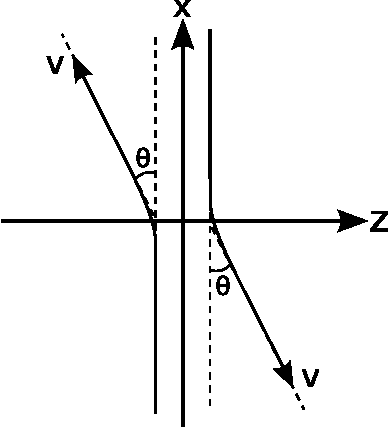
\includegraphics[scale=0.8]{images/TouschekScatter}
	\caption[Touschek scattering in the centre of mass of the bunch]{Touschek scattering in the centre of mass of the bunch. Momentum is transferred from the $x$-direction (transverse) to the $z$-direction (longitudinal). In this figure, the bunch is travelling in the $z$ direction \cite{Wolski}.}
	\label{fig:TousScat}
\end{figure}

	The Touschek effect is a scattering effect that occurs between particles in the same bunch. Particles in a bunch undergo large angle Coulomb collisions, which transfers momentum to the longitudinal plane. This can force particles out of the momentum acceptance of the ring, causing the particles to be lost. Touschek lifetime, $\tau_{T}$, is given by:
\begin{equation}
	{\frac{1}{\tau_{T}} = -\frac{1}{N_{b}}\frac{dN_{b}}{dt} \propto -\frac{N_{b}}{\sigma_{y}}}
	\label{eqn:touschekEqn}
\end{equation}
where $N_{b}$ is the number of particles in a bunch, $\sigma_{y}$ is the vertical beam size, and $dN_{b}/dt$ is the loss rate of the beam \cite{Wolski}. As shown in Table~\ref{tab:SKBBEAM}, the horizontal beam size is much larger than the vertical beam size, and as such it remains roughly constant. During the machine studies, the number of particles in a beam was not measured, but the number of bunches in the whole ring was. This can be related to the number of particles in each bunch using the relationship:
\begin{equation}
	{N_{b} \propto\frac{I}{N_{\mathrm{Bunch}}}}
\end{equation}
where $N_{\mathrm{Bunch}}$ is the number of bunches in the entire ring, and $I$ is the beam current. Substituting this into Eqn \ref{eqn:touschekEqn} gives:
\begin{equation}
	{\frac{dI}{dt}\propto-\frac{I^2}{N_{\mathrm{Bunch}}\sigma_{y}}}
\end{equation}


%\section{Other interactions}

%collision with dust

%electron cloud effect

\section{Radiative Bhabhas}

Radiative Bhabhas (RBB) occur when an electron and positron scatter off each other, with one or both particles emitting a photon. This photon can cause showers of electrons and photons in the detector. For low angle scattering, some particles will be knocked out of stable orbit and can be scattered into the detector, producing more showers. These showers can lead to degradation in the performance of the detector. This was not an issue in Phase~I of BEAST~II since there were no collisions.

\section{Neutron Production}

%	It is not immediately obvious how the neutrons that the \he tubes will measure are produced, since SuperKEKB is an \epem accelerator, and neutrons are hadrons. 


The neutrons that the \he tubes measured are produced by bremsstrahlung photons (note that this refers not only to the bremsstrahlung discussed in \S~\ref{sec:brem}, but also to bremsstrahlung of electrons interacting with other materials near the beam, such as the beampipe) producing photo nuclear reactions. Beam-gas, Touschek, and RBB events cause electrons to be knocked out of stable orbits, which leads to collisions with the beampipe walls, producing the bremsstrahlung photons that then produce neutrons. These neutrons are produced with a large energy distribution, with a threshold between 4 and 20 MeV. As these neutrons travel through various materials, they become thermalized \cite{PDGBook}.




% There is a process called the giant dipole resonance that is responsible for producing neutrons in \epem accelerators. A photon's electric field collectively excites the nucleus of an atom (in the beampipe, or any other structure nearby), causing the protons and neutrons in the nucleus to oscillate. This oscillation is quickly damped by friction. 












































\chapter{Machine Study Experiments}
\label{chap:machStudies}

\section{Introduction}

	Phase~I of BEAST~II occurred February 15 -- June 29 2016, during which the electron and positron beams were circulated in closed orbits around the SuperKEKB syncrotron but were not brought into collision. The rates in the \he tubes during Phase~I are shown in Fig \ref{fig:RateAll}.  In May, there were several periods of special machine experiments, where the beam conditions were set to study various background effects. These machine experiments included:  increasing the pressure of the gas in the beampipes, changing the size of the beams, varying the current in the beams, changing the size of the collimators in the beampipes, and studying the injection backgrounds.



\begin{figure}[htb]
	\centerfloat
		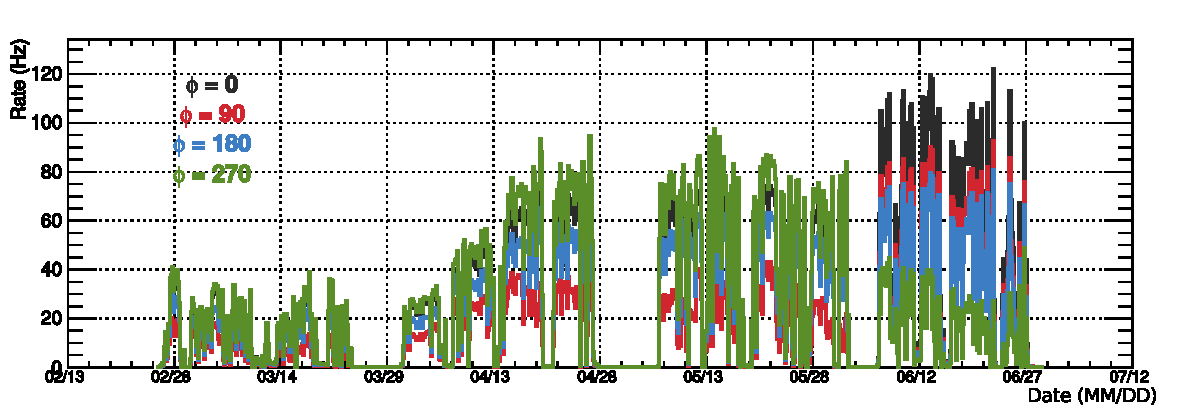
\includegraphics[trim={0 0 0 0.3cm},clip, width=\textwidth]{images/Rate_AllPhaseI}
	\caption[\He tube rates throughout BEAST~II Phase~I]{\He tube rates throughout BEAST~II Phase~I. The tubes located at $\phi=90$ and $\phi=270$ were swapped on June 1st.}	
	\label{fig:RateAll}
\end{figure}




\section{Pressure Experiments}


	To study the beam-gas interactions, the pressure in the beampipe was increased at various locations around the accelerator ring. These locations are shown in Fig \ref{fig:SKBVac}. Fig \ref{fig:VacuumBumpEg} shows an example of how the pressure at one of these locations changed with time.

\begin{figure}[htb]
	\centerfloat
		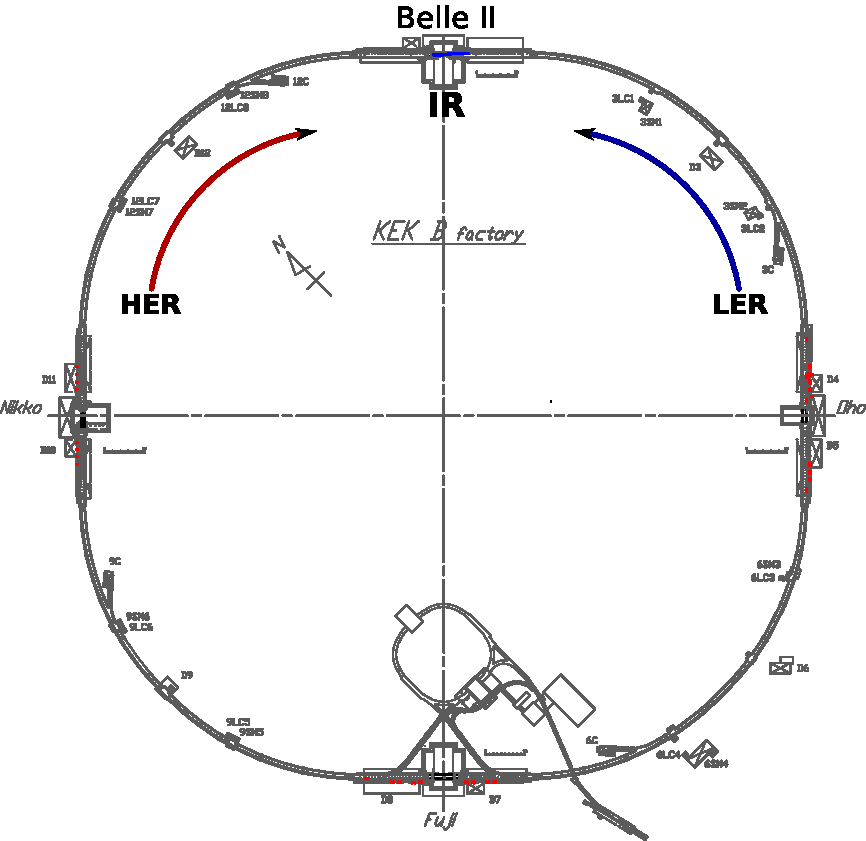
\includegraphics[scale=0.6]{images/SKEKb_key}

		\begin{picture}(2,2)
			\put(20,240){\color{blue}\thicklines\circle{20}}
			\put(110,135){\color{blue}\thicklines\circle{20}}
			\put(25,30){\color{blue}\thicklines\circle{20}}
			\put(-100,135){\color{blue}\thicklines\circle{20}}
	
			\put(80,210){\color{red}\thicklines\circle{20}}
			\put(-70,210){\color{red}\thicklines\circle{20}}
			\put(110,135){\color{red}\thicklines\circle{22}}
			\put(25,30){\color{red}\thicklines\circle{22}}
			\put(105,60){\color{red}\thicklines\circle{20}}
			\put(-70,60){\color{red}\thicklines\circle{20}}
		\end{picture}
	\caption[Locations of pressure increases]{Locations of pressure increases. LER locations are circled in blue, and HER locations are circled in red~\cite{SKBgroup}.}
	\label{fig:SKBVac}
\end{figure}

\begin{figure}[htb]
	\centerfloat
		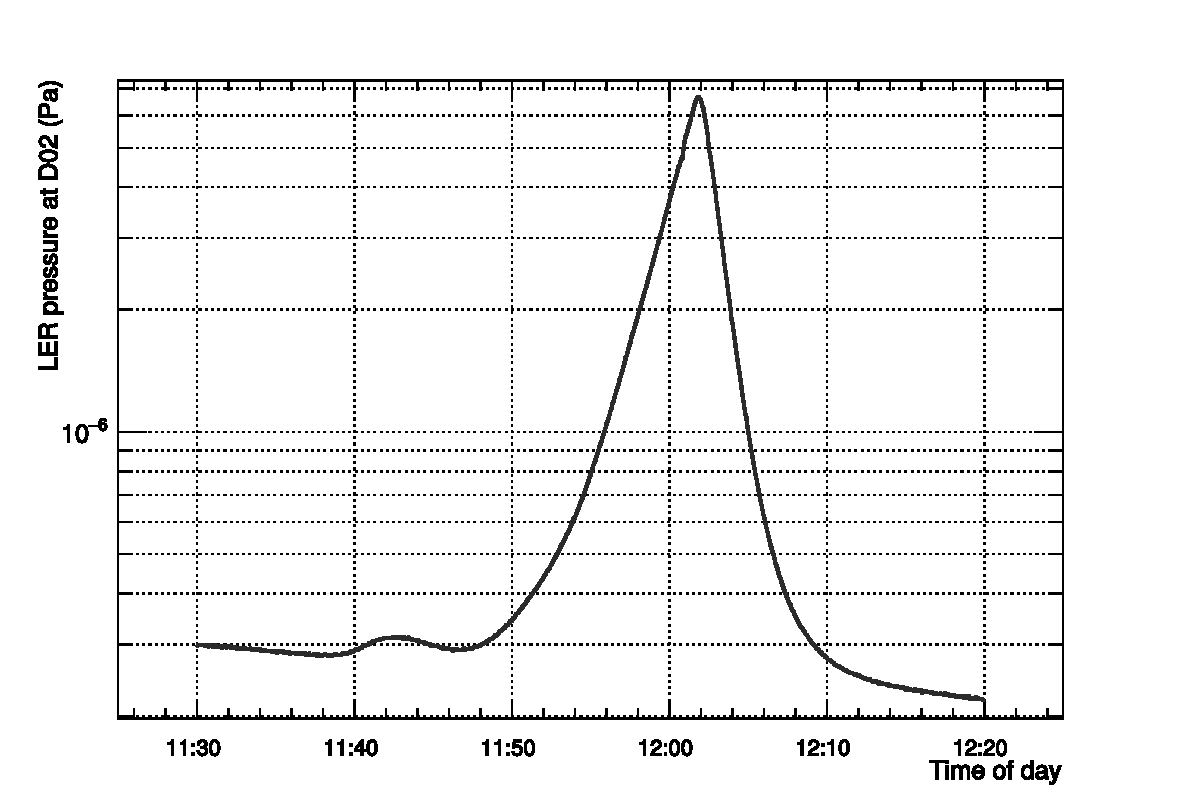
\includegraphics[trim={0 0 0 0.75cm},clip, width=\textwidth]{images/PressureBump}
	\caption[Example of pressure change during vacuum bump study]{Example of pressure change during vacuum bump study. Horizontal axis is log scale. Note the double bump. Data were recorded on May 23, 2016.}	
	\label{fig:VacuumBumpEg}
\end{figure}


	To reduce the beampipe pressure to an adequate vacuum level, Non-Evaporable Getter (NEG) pumps were used. These reduce the pressure by absorbing residual gas molecules in the beampipe. During the pressure bump studies, the NEGs at various locations around the beam were heated. This released the captured gas molecules back into the beampipe, increasing the pressure. The heating was done in two stages, which is the cause of the two bump structures seen in Fig \ref{fig:VacuumBumpEg}. 


\section{Touschek Experiments}



\begin{figure}[htb]
	\centerfloat
		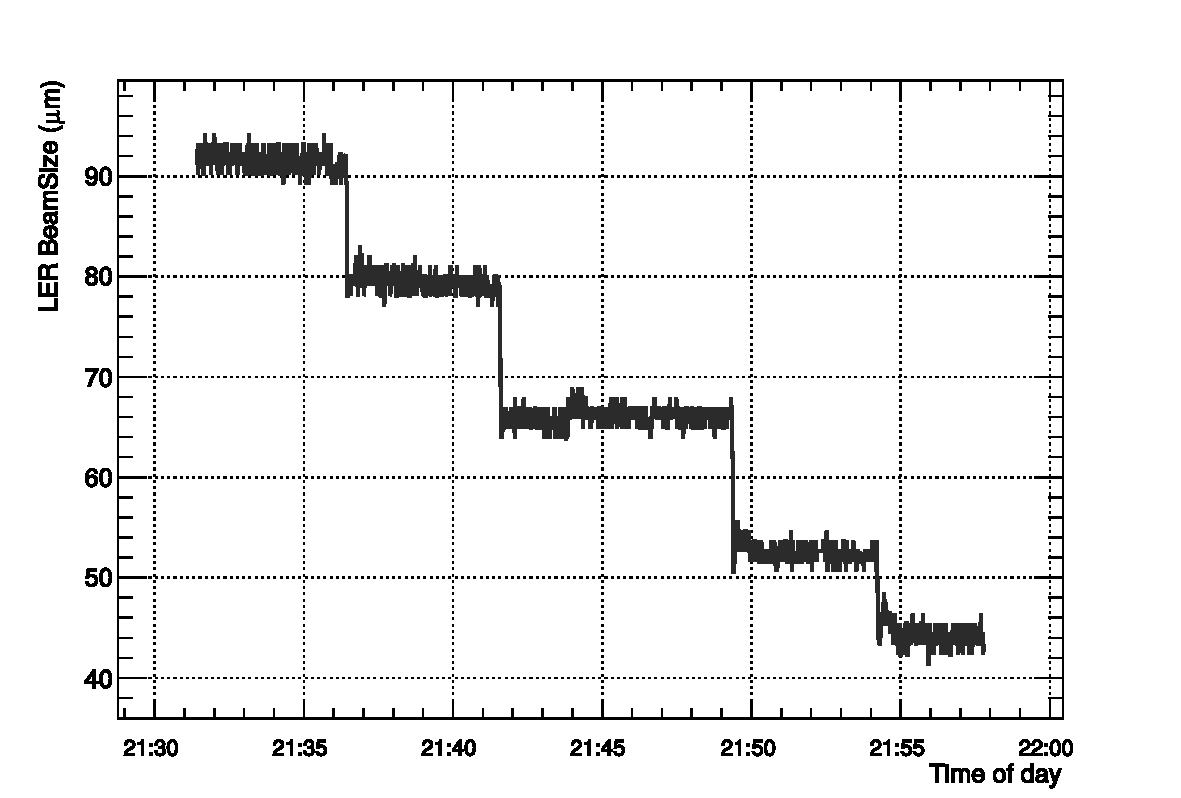
\includegraphics[trim={0 0 0 0.75cm},clip, width=\textwidth]{images/BeamSizeScan}
	\caption[Example of beam size change during beam size scan]{Example of beam size change during beam size scan. Data were recorded on May 17, 2016.}	
	\label{fig:BeamSizeEg}
\end{figure}


	To examine the Touschek contribution to the beam backgrounds, runs were taken where the size of the beam was varied. At each beam size setting, current was injected and allowed to decay over a period of time. An example of how the beam size changed during one of these runs is given in Fig \ref{fig:BeamSizeEg}.

	
	Different approaches were used to change the beam size in the LER and HER beams. In the LER, the x-y coupling of the beam was increased by changing the strength of some of the quadrupole magnets. This increased the vertical beam size without changing the beam orbit. This was attempted in the HER, but the change in beam size was not as dramatic as desired. Instead, the beam orbit at one of the bending magnets was adjusted, which increased the vertical dispersion and horizontal size. The beam orbit outside these bending magnets was unchanged~\cite{Hiro}.





\section{Vacuum Scrubbing}


	The beampipe walls contain gas molecules that were absorbed during manufacturing, shipping, etc. When beams are run through the beampipe, these molecules are desorbed from the surface of the beampipes by photons produced by the beams \cite{chao2013handbook}. Figure \ref{fig:LERPRECUR} shows the current and pressure in the LER beam as a function of time. When the LER current increases, the pressure also increases due to the desorption of gas molecules.

	As more beam is passed through the rings, there is less and less gas to be desorbed --- the beampipes get cleaner. This should manifest as a decrease in $dP/dI$, the change in pressure per change in current. This quantity is known as the dynamic pressure. The event rate measured in BEAST~II detectors should also decrease.



%	Most of Phase~I was vacuum scrubbing. In order to reduce the gas pressure in the beampipe, the particle beam is run with a large beam size. This causes the beampipe walls to expel the gas molecules they have absorbed. These gas molecules are then pumped out by the NEGs. 

%discussion of dP/dI


\begin{figure}[htb]
	\centerfloat
		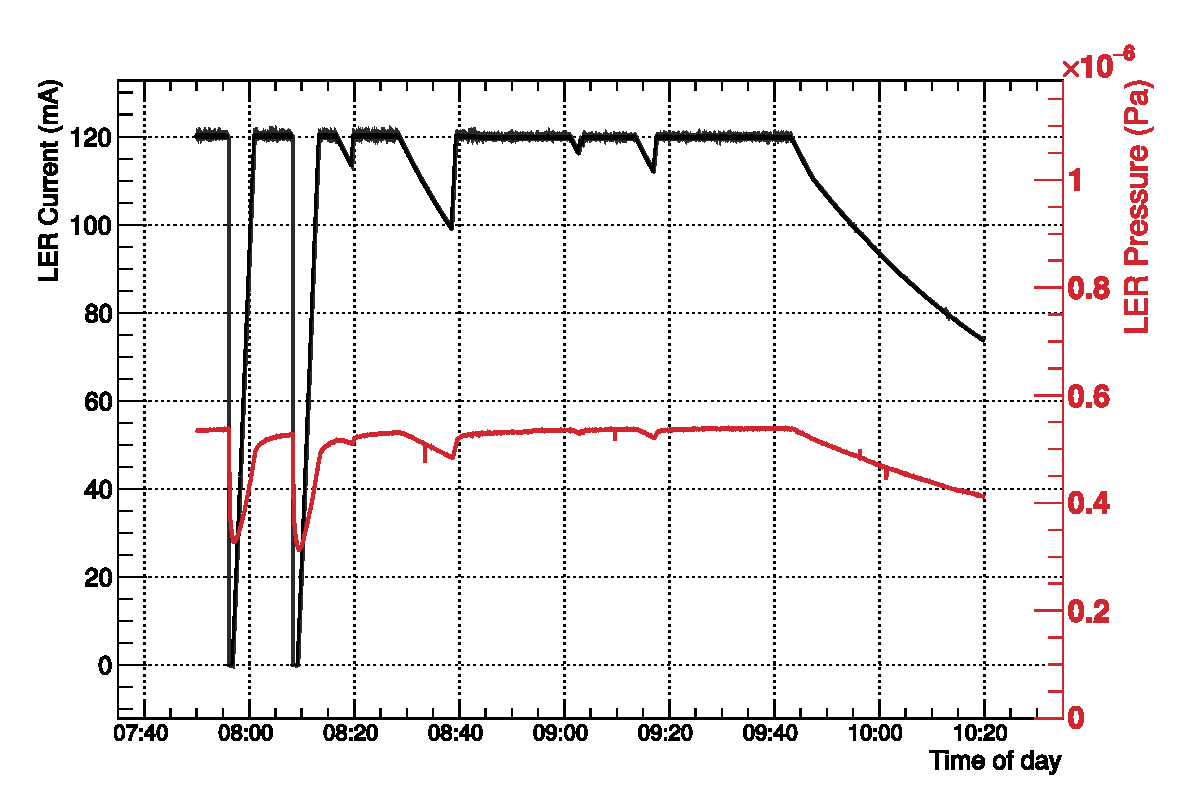
\includegraphics[trim={0 0 0 0.75cm},clip, width=\textwidth]{images/LER_PreAndCur}
	\caption[Example of LER current and pressure during vacuum scrubbing]{Example of LER current and pressure during vacuum scrubbing. When the beam current increases, the pressure increases too. Black is the beam current, and red is the beampipe pressure. Data were recorded on March 3, 2016.}
	\label{fig:LERPRECUR}
\end{figure}



\subsection{Analysis}


	During most of the vacuum scrubbing, both the HER and LER beams were running. In order to separate the effect of each beam, the average of the rates in the four \he tubes is fit to:
\begin{equation}
	{R_{^{3}\mathrm{He tube}} = A_{\mathrm{HER}} (P\cdot I)_{\mathrm{HER}}+A_{\mathrm{LER}} (P\cdot I)_{\mathrm{LER}}}
	\label{eqn:vacScrbModel}
\end{equation}
where $(P\cdot I)$ is the pressure times current for each beam. This model is very simple as it ignores any Touschek component, which is proportional to $I^2/(N_{\mathrm{Bunch}}\sigma_{y})$. During the scrubbing, the beam size was generally quite large, so the Touschek component would be small. Eqn \ref{eqn:vacScrbModel} can be be separated into the HER and LER components:
\begin{subequations}
\begin{align}
		{R_{\mathrm{HER}} = A_{\mathrm{HER}} (P\cdot I)_{\mathrm{HER}}} \\
		{R_{\mathrm{LER}} = A_{\mathrm{LER}} (P\cdot I)_{\mathrm{LER}}}
\end{align}
\end{subequations}
Figure \ref{fig:VacScrbExample} shows an example of this fit for one day of running.

\begin{figure}
	\centerfloat
		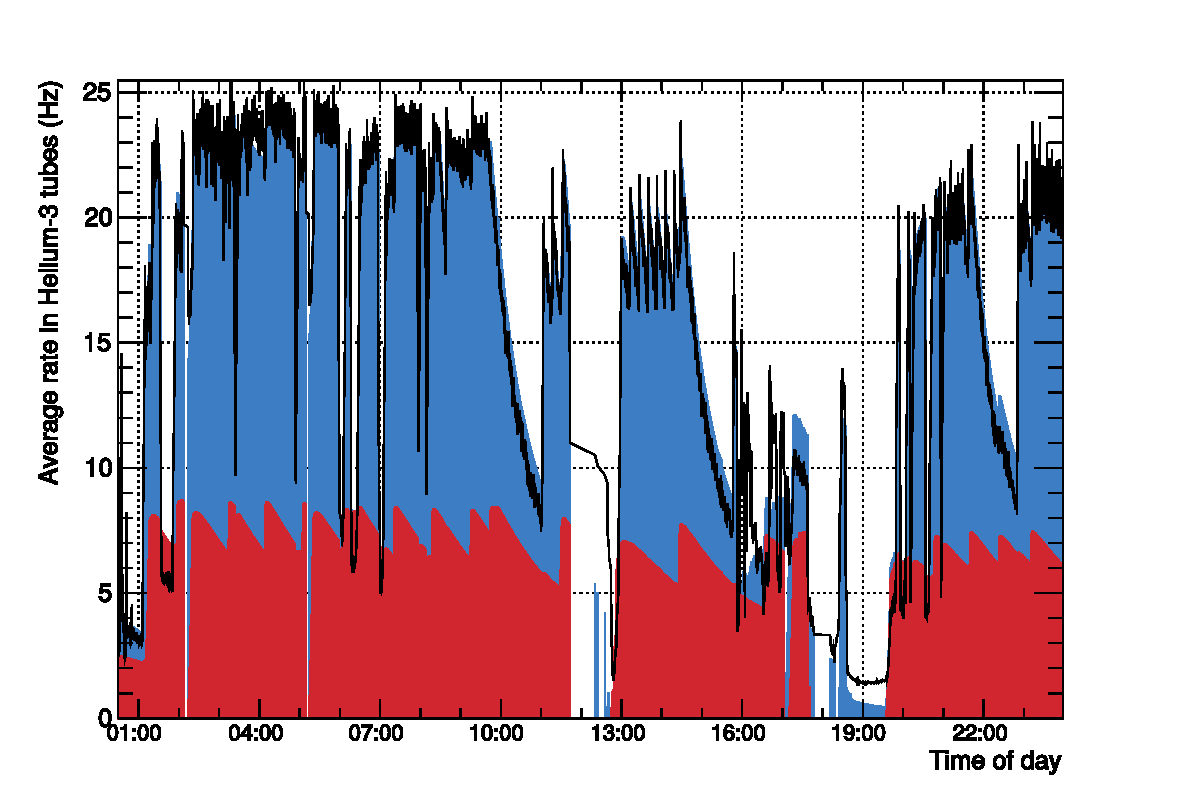
\includegraphics[trim={0 0 0 0.7cm},clip, width=\textwidth]{images/VacuumScrubFitExample}
	\caption[Fitting example for vacuum scrubbing]{Fitting example for vacuum scrubbing. Blue is the LER fit, red is the HER fit, and black is the average rate in the \he tubes. Data were recorded on March 3, 2016.}	
	\label{fig:VacScrbExample}
\end{figure}


The fit was recalculated for each day that data were taken. A requirement that both beams have at least 30 mA of current was applied. The rate was normalized by current squared. An average value of $R/I^2$ was calculated for each beam on each day of running, removing any days when the beams were off, or when the machine study experiments were being conducted. These daily values are plotted against the integrated current on the same day (see Fig \ref{fig:VacScrb}).

	The dynamic pressure $dP/dI$ as a function of the integrated current follows a power law of the form \cite{chao2013handbook}:
\begin{equation}
	{\frac{dP}{dI}\propto \left(\int{Idt}\right)^{-k}}
\end{equation}
$dP/dI$ is also plotted in Fig \ref{fig:VacScrb}, using data from \cite{SKBVacuum}. Both $R/I^2$ and dP/dI are fit to a power law, with the fit values shown in Table \ref{tab:PowerLawFits}. The parameters k for $R/I^2$ and $dP/dI$ are within 2$\sigma$ of each other, for both HER and LER, which shows that the effect of the vacuum scrubbing is observed with the \he tubes.


\begin{figure}
	\centering
	\subfigure[LER]{
		\begin{overpic}[trim={0 0 0 0.75cm},clip, width=\textwidth]{images/LER_withdPdI}
		\end{overpic}
		\label{fig:LERVacScrb}
	}
	\subfigure[HER]{
		\begin{overpic}[trim={0 0 0 0.75cm},clip, width=\textwidth]{images/HER_withdPdI}
		\end{overpic}
		\label{fig:HERVacScrb}
	}
	\caption[Vacuum scrubbing during BEAST~II Phase~I]{Vacuum scrubbing during BEAST~II Phase~I. Black is the dynamic pressure $dP/dI$ in each beam, and red or blue is the average rate of all four \he tubes, plotted against the integrated current. The \he tube follows the same trend as the dynamic pressure.}	
	\label{fig:VacScrb}
\end{figure}

\begin{table}
	\centering
	\begin{tabular}{ ccccc }
		&	\multicolumn{2}{c}{\He tubes}	& \multicolumn{2}{c}{$dP/dI$}					\\
  		& Constant (Hz/mA$^2$) 			& k		& Constant (Pa/mA) 		& k		\\\hline \hline
	LER	& (10.5$\pm$2)$\times10^{-3}$		& 0.81$\pm$0.04	& (16.9$\pm$2)$\times10^{-5}$	& 0.74$\pm$0.02	\\ 
	HER	& (8.0$\pm$1.4)$\times10^{-3}$		& 0.85$\pm$0.03	& (4.13$\pm$0.4)$\times10^{-5}$	& 0.89$\pm$0.02	\\ \hline

	\end{tabular}
	\caption[Power law fits for \he tube rate and $dP/dI$]{Power law fits for \he tube rate and $dP/dI$.}
	\label{tab:PowerLawFits}
\end{table}






























\chapter{Simulation}
\label{chap:Sim}

	Simulation of the collider was done with a software package called Strategic Accelerator Design (SAD) \cite{SAD}, created at KEK specifically for simulating \epem colliders. SAD simulates the loss of particles from both the HER and LER beams, for beam-gas and beam-beam losses. The trajectory of particles lost at the IR are passed to the Belle~II Analysis Framework (BASF2) \cite{BASF2}. 

	The information passed to BASF2 is propagated through the materials and detectors in the IR using GEANT4. GEANT4 simulates the interaction with detector materials, calculating the energy deposited in the detector materials. These energy deposits are converted into digitized signals using code specifically developed for each subdetector.

\section{Scaling of Simulation}

%discuss scaling of simulation to data. Need to understand better.


\begin{table}[htb]
	\centering
	\begin{tabular}{ cccccccc }
	Ring	& Current & Pressure 	& Z & N$_{\mathrm{bunch}}$	& $\sigma_y$ 		& emittance ($\varepsilon_x$) 	& $\varepsilon_y/\varepsilon_x$ \\
		& (mA)	  & (nTorr)	&   & 				& ($\mu\mathrm{m}$)	& (mm$\times$mrad)	&  \\ \hline \hline
	HER	& 1000		& 10			& 7 & 1000		& 59		& 4.45		& 0.1	\\
	LER	& 1000		& 10			& 7 & 1000		& 110		& 1.92		& 0.1	\\	\hline
	\end{tabular}
	\caption[Nominal parameters of simulated beams]{Nominal parameters of simulated beams.}
	\label{tab:SimBeam}
\end{table}


The SAD simulation was done with the beam parameters listed in Table \ref{tab:SimBeam}. 


The beam-gas and beam-beam components of the background are simulated separately. Each component is then scaled to match the real beam parameters by re-weighting the SAD events by the scale value at that moment in time. The same SAD events are reused for all beam settings.

The beam-gas component of the simulation is scaled by:
\begin{equation}
	{R_{\mathrm{BG}}^{\mathrm{Scaled}} = \sum _{i=1}^{12}(R^{\mathrm{Brems}}_i+R^{\mathrm{Coulomb}}_i)\cdot\frac{P_{\mathrm{scale}}(I\cdot P_i\cdot Z_{\mathrm{eff}~i}^{2})_{\mathrm{data}}} {(I\cdot P\cdot Z^{2})_{\mathrm{sim}}}}
\end{equation}
where $R^{\mathrm{Brems}}_{i}$ and $R^{\mathrm{Coulomb}}_{i}$ are the components of the inelastic and elastic beam-gas simulated rates produced at the IR from interaction at each `D' section of the HER and LER rings (see Fig \ref{fig:SKB}), $P_{i}$ is the pressure in each `D' section, and $Z_{\mathrm{eff}~i}$ is the effective atomic number of the gas in each section (see Eqn~\ref{eqn:ZEFF}), if available. If $Z_{\mathrm{eff}~i}$ is not available in a `D' section, 2.7 is used for the LER (since this was near the mean value of $Z$ during the experiment, see \S~\ref{sec:TousExp}), and 1 is used in the HER.  $P_{\mathrm{scale}}$ is a scale factor on the overall pressure to account for the fact that the measurement made by the uncalibrated pressure gauges is proportional to the actual pressure. This scale factor will be discussed further in \S~\ref{sec:TousExp}.

The beam-beam component of the simulation is scaled by:
\begin{equation}
	{R_{\mathrm{Tous}}^{\mathrm{Scaled}} = R_{\mathrm{Tous}}\cdot\frac{(I^{2}/N_{\mathrm{Bunch}}\cdot\sigma_{y})_{\mathrm{data}} }{(I^{2}/N_{\mathrm{Bunch}}\cdot\sigma_{y})_{\mathrm{sim}}}}
\end{equation}
where $R_{\mathrm{Tous}}$ is the Touschek simulated rate, $\sigma_{y}$ is the beam size, and $N_{\mathrm{Bunch}}$ is the number of bunches in the ring.

These scaled components are combined to get the re-weighted simulated rate:
\begin{equation}
	{R_{\mathrm{Sim}} = \varepsilon_{^3\mathrm{He}}\left(R_{\mathrm{BG}}^{\mathrm{Scaled}}+R_{\mathrm{Tous}}^{\mathrm{Scaled}}\right)}
\end{equation}
where $\varepsilon_{^3\mathrm{He}}$ is the efficiency in each \he tube, as shown in Table \ref{tab:he3Calib}. The scaling parameters for the beam-gas and beam-beam backgrounds are consistent with the discussion in Chapter \ref{chap:beamBack}.


%In order to simulate the differing conditions of the machine studies, this simulation was scaled:
%\begin{equation}
%	{R = \varepsilon_{^3He}\left(\sum _{i=1}^{12}(R^{Brems}_i+R^{Coulomb}_i)\cdot\frac{P_{\mathrm{scale}}(I\cdot P_i\cdot Z_{i}^{2})_{data}} {(I\cdot P\cdot Z^{2})_{sim}}+R_{Tous}\cdot\frac{(I^{2}/N_{Bunch}\cdot\sigma_{y})_{data} }{(I^{2}/N_{Bunch}\cdot\sigma_{y})_{sim}}\right)}
%\end{equation}
% R$_{Tous}$ is the Touschek simulated rate. Finally, $\varepsilon_{^3He}$ is the efficiency in each \he tube, as shown in Table \ref{tab:he3Calib}. The scaling parameters are consistent with the discussion on Chapter \ref{chap:beamBack}

In order to verify that these scale factors are appropriate, a SAD simulation was done at different beam parameters than listed in Table \ref{tab:SimBeam}. This was compared to a scaled version of the nominal simulation, which showed this scaling approach to be appropriate.



\section{\He Tube simulation}

	The \he tube geometry, which consists of a stainless steel cylinder 8$^{\verb+"+}$ long and 2$^{\verb+"+}$ in diameter, filled with $^3$He, is loaded into GEANT4. The GEANT4 physics list QGSP\_BERT\_HP (a hadronic model with a high precision neutron package) is used to determine if a neutron passing through the detector's sensitive volume is captured by an atom of $^3$He. When this occurs, a tritium and a proton are produced. These particles travel through simulated trajectories, and ionization sites in the $^3$He are generated. If the energy deposited in one of these sites is greater than the ionization energy of $^3$He (24.6 eV), the number of electrons generated is calculated by dividing the energy of the event by the ionization energy. This number is smeared by a Gaussian function, and converted to ADC counts. If this is above a certain threshold, the hit is counted toward the rate. 






















\chapter{Analysis}
\label{chap:Anal}




\section{Pressure Experiments}
\label{sec:PBump}

The response in the \he tubes during one of the pressure bump runs can be found in Fig~\ref{fig:rateVsTimeVacuum}. Fig~\ref{fig:rateVsTimeVacuum}(a) shows $P\cdot I$ during the run, Fig~\ref{fig:rateVsTimeVacuum}(b) shows the response in the four \he tubes during the run, Fig~\ref{fig:rateVsTimeVacuum}(c) shows $P\cdot I\cdot Z_{\mathrm{eff}}^2$, and Fig~\ref{fig:rateVsTimeVacuum}(d) shows $Z_{\mathrm{eff}}$. Figs~\ref{fig:rateVsTimeVacuum}(c) and~\ref{fig:rateVsTimeVacuum}(d) will be discussed further in \S~\ref{sec:massSpec}. Fig~\ref{fig:rateVsTimeVacuumlog} shows the same plots as Fig~\ref{fig:rateVsTimeVacuum}, with a log scale to emphasize double bump structure.

\begin{figure}
	\centerfloat
		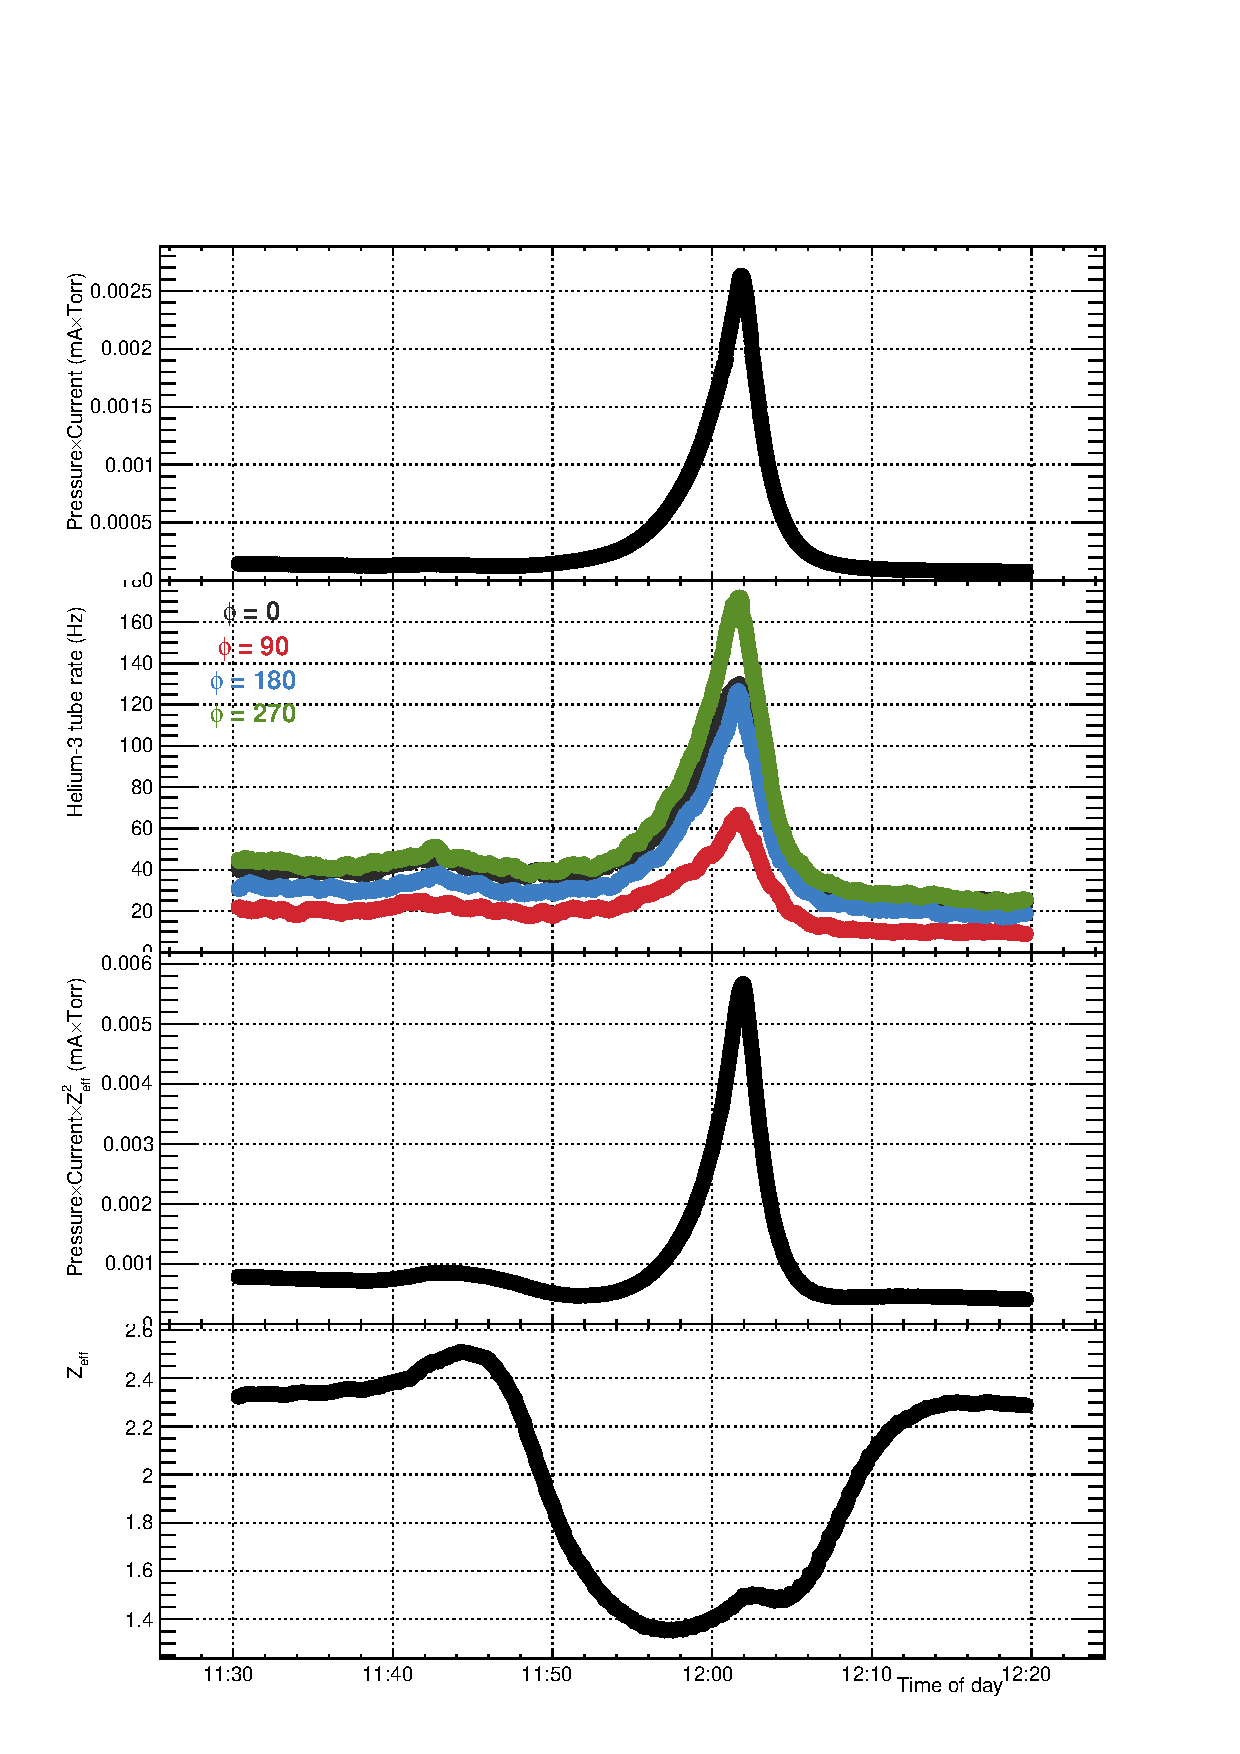
\includegraphics[width=\textwidth]{images/MassSpecCombined}
		\begin{picture}(2,2)
			\put(-100,500){(a)} %1
			\put(-100,380){(b)} %1
			\put(-100,250){(c)} %1
			\put(-100,120){(d)} %1
		\end{picture}
	\caption[Response in \he tubes during vacuum bump run]{Response in \he tubes during vacuum bump run. Data were recorded on May 23, 2016.}	
	\label{fig:rateVsTimeVacuum}
\end{figure}

\begin{figure}
	\centerfloat
		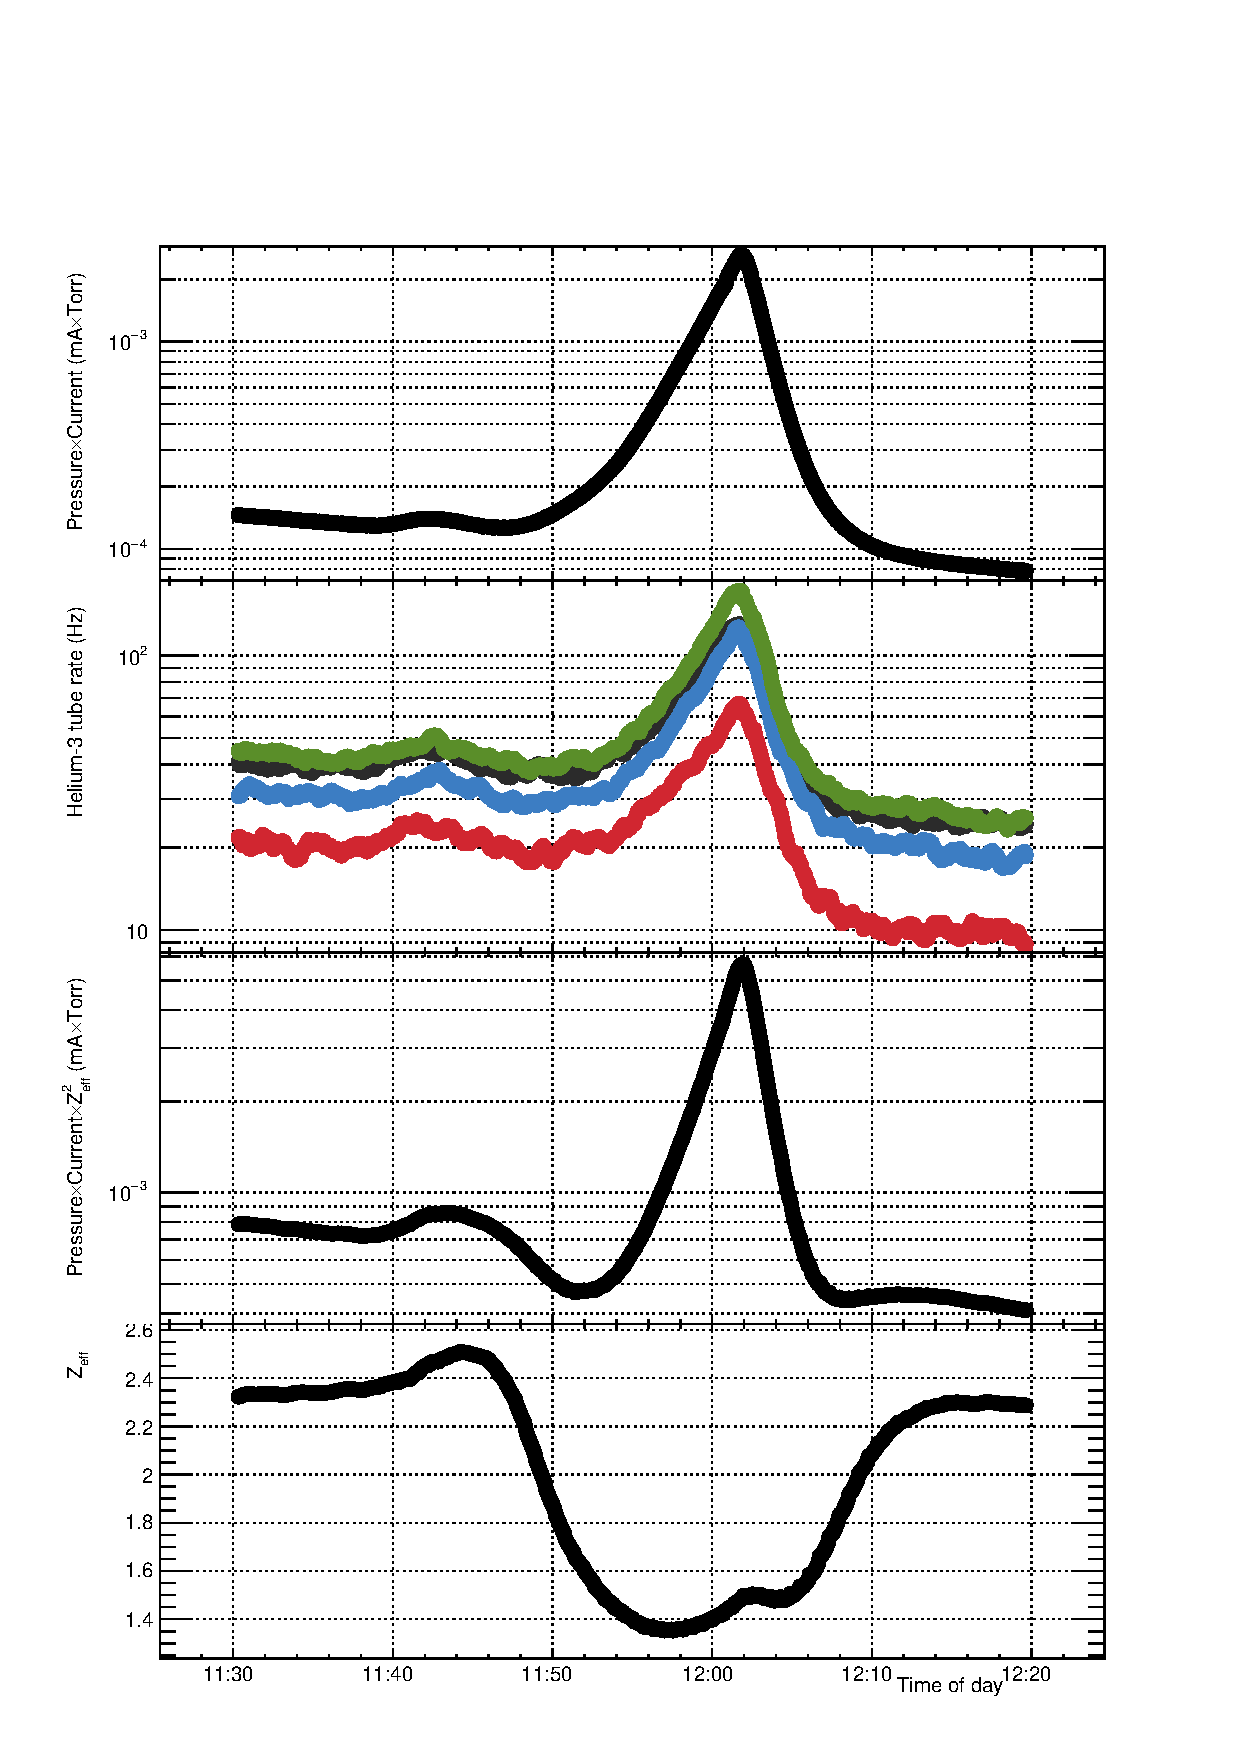
\includegraphics[width=\textwidth]{images/MassSpecCombined_log}
		\begin{picture}(2,2)
			\put(-100,500){(a)} %1
			\put(-100,380){(b)} %1
			\put(-100,250){(c)} %1
			\put(-100,120){(d)} %1
		\end{picture}
	\caption[Response in \he tubes during vacuum bump run, log scale]{Response in \he tubes during vacuum bump run, log scale. Data were recorded on May 23, 2016.}	
	\label{fig:rateVsTimeVacuumlog}
\end{figure}

\paragraph{Smoothing of data}

	Before the analysis of the pressure bumps was done, the data were smoothed using this equation:
\begin{equation}
	{R_{i} = \frac{1}{2n+1}\sum_{j=i-n}^{j=i+n}R_{j}}
\end{equation}
where $R_j$ is the \he tube rate in a one second time bin $j$. This algorithm takes the average of the previous $n$ time bins, the current bin, and the next $n$ bins. For the studies presented here, $n=20$ was used. An example showing the rate in the \he tubes is shown in Fig~\ref{fig:smoothPlot}. This smoothing was done to reduce the fluctuations of the signal. Since this smoothing will reduce the height of the maximum, only the data from the rising portion of the experiment were analysed.

\begin{figure}
	\centering
	\subfigure[Channel 0 ($\phi=0^{\circ}$)]{
		\begin{overpic}[trim={0 0 0 0.5cm},clip, width=0.47\textwidth]{images/SmoothingPlot0}
		\end{overpic}
		\label{fig:smoothPlot0}
	}
	\subfigure[Channel 1 ($\phi=90^{\circ}$)]{
		\begin{overpic}[trim={0 0 0 0.5cm},clip, width=0.47\textwidth]{images/SmoothingPlot1}
		\end{overpic}
		\label{fig:smoothPlot1}
	}
	\subfigure[Channel 2 ($\phi=180^{\circ}$)]{
		\begin{overpic}[trim={0 0 0 0.5cm},clip, width=0.47\textwidth]{images/SmoothingPlot2}
		\end{overpic}
		\label{fig:smoothPlot2}
	}
	\subfigure[Channel 3 ($\phi=270^{\circ}$)]{
		\begin{overpic}[trim={0 0 0 0.5cm},clip, width=0.47\textwidth]{images/SmoothingPlot3}
		\end{overpic}
		\label{fig:smoothPlot3}
	}
	\caption[Smoothing of \he tube data for pressure bump studies]{Smoothing of \he tube data for pressure bump studies where $n=20$. Grey is the unsmoothed data, red is the smoothed data. Data were recorded on May 23, 2016.}
	\label{fig:smoothPlot}
\end{figure}




\subsection{Gas Model Using Beampipe Pressure}

	Initially a simple gas model was used to characterize the response. In this model, it is assumed that the beam-gas cross section is proportional to the pressure in the beampipe. In Fig~\ref{fig:rateVsPressCur}, the rate in the \he tubes is plotted as a function of current times pressure. Only the rising portion of the bumps is plotted, corresponding to time (HH:MM) ranges of 11:40-11:45 for the first bump, and 11:50-12:02 for the second bump. Data are binned in 1 second time bins.


\begin{figure}
	\centering
	\subfigure[Channel 0 ($\phi=0^{\circ}$)]{
		\begin{overpic}[trim={0 0 0 0.5cm},clip, width=0.47\textwidth]{images/HE3_0_withoutMassSpec}
		\end{overpic}
		\label{fig:rateVsPressCur0}
	}
	\subfigure[Channel 1 ($\phi=90^{\circ}$)]{
		\begin{overpic}[trim={0 0 0 0.5cm},clip, width=0.47\textwidth]{images/HE3_1_withoutMassSpec}
		\end{overpic}
		\label{fig:rateVsPressCur1}
	}
	\subfigure[Channel 2 ($\phi=180^{\circ}$)]{
		\begin{overpic}[trim={0 0 0 0.5cm},clip, width=0.47\textwidth]{images/HE3_2_withoutMassSpec}
		\end{overpic}
		\label{fig:rateVsPressCur2}
	}
	\subfigure[Channel 3 ($\phi=270^{\circ}$)]{
		\begin{overpic}[trim={0 0 0 0.5cm},clip, width=0.47\textwidth]{images/HE3_3_withoutMassSpec}
		\end{overpic}
		\label{fig:rateVsPressCur3}
	}
	\caption[Rate in \he tubes vs pressure times current in LER beam]{Rate in \he tubes vs pressure times current in LER beam. Blue corresponds to the larger pressure increase occurring from 11:50 to 12:02 and orange corresponds to the small pressure increase occurring from 11:40 to 11:45.}	
	\label{fig:rateVsPressCur}
\end{figure}




	As evident from Fig~\ref{fig:rateVsPressCur}, the response due to the first bump is quite different from the response due to the second bump. The simple gas model that assumes that the beam-gas rate is proportional to $P\cdot I$ does not adequately describe what is happening in this data. A more complex gas model is necessary.



\subsection{Gas Model Using Mass Spectrum Data}
\label{sec:massSpec}


	The elastic and inelastic cross sections of beam particles interacting with gas in the beampipe are given by Eqns~\ref{eqn:coulomb} and~\ref{eqn:brems}. Both cross sections are approximately proportional to $Z^2$, where $Z$ is the number of protons in the target. If the gas composition in the beampipe does not change, $Z^2$ will be constant, and the change in beampipe pressure alone is sufficient to determine the beam-gas cross section. If it is known that the gas composition is changing, however, simply using pressure will produce different responses as seen in Fig~\ref{fig:rateVsPressCur}. Therefore a more complex gas model is necessary.


\subsubsection{Mass Spectrum Fit}

	The SuperKEKB collider has two residual gas analysers (RGAs) on the LER beampipe, located at D02 and D06 (see Fig~\ref{fig:SKBVac}). These devices are simple mass spectrometers, which measure the partial pressure for mass-to-charge ratio (m/z) values from 1 to 50 (m is number of nucleons in a molecule `fragment', z is the charge of the `fragment', so m/z has no units). Using this information, it is possible to infer the composition of the gas in the beampipe. 


\begin{table}
	\centering
	\begin{tabular}{ cc }
		Molecule Name	& Number of protons	\\	\hline \hline
		$H_2$		& 2		\\	
		$D_2$		& 2		\\	
		$DH$		& 2		\\	
		$H_{2}O$	& 10		\\	
		$H_{3}N$	& 10		\\	
		$CH_4$		& 10		\\	
		$CO$		& 14		\\	
		$C_{2}H_4$	& 16		\\	
		$Ar$		& 18		\\	
		$C_{2}H_6$	& 18		\\	
		$CO_2$		& 22		\\	
		$C_{3}H_4$	& 22		\\	
		$C_{3}H_6$	& 24		\\	
		$C_{3}H_8$	& 26		\\ \hline
	\end{tabular}
	\caption[Molecules used in fit to RGA data]{Molecules used in fit to RGA data.}
	\label{tab:Molecules}
\end{table}


	Using mass spectra data taken from the National Institute of Standards and Technology (NIST) database \cite{nistMassSpec}, the spectra of various molecules were fit to the data measured by the RGA. A list of the gases used in the fit is given in Table~\ref{tab:Molecules}, and example spectra of the most prominent molecules present in the beampipe are shown in Fig~\ref{fig:ExampleMassSpecs}. 

The mass spectrum measured by the RGA is a linear sum of the mass spectra from all the gases that make up the gas mixture in the beampipe \cite{MassSpecBook}:
\begin{equation}
	{\vec{S}^{\mathrm{Measured}} = \sum_{i=1}^{n_{\mathrm{molecules}}}p_{i}\vec{S}^{\mathrm{Template}}_{i} \equiv \textbf{S}^{\mathrm{Template}}\vec{p}}
\end{equation}
where $\vec{S}^{\mathrm{Measured}}$ is a vector containing the data measured by the RGA (the partial pressure for m/z from 1 to 50, shown in black in Fig~\ref{fig:mSpecFit}), $\vec{S}_{i}^{\mathrm{Template}}$ is a vector containing the spectrum of a molecular species spectrum (for example, H$_2$O as in Fig~\ref{fig:exampleH2O}), and $p_{i}$ is the partial pressure of that species, which is extracted from the fit. This is equivalent to a matrix equation, where $\vec{p}$ is a vector containing the partial pressure of each gas species, and $\textbf{S}^{\mathrm{Template}}$ is a matrix with the mass spectra vectors $\vec{S}_{i}^{\mathrm{Template}}$ as the columns. To find the partial pressure of each gas species, a least squares analysis is used, the solution to which is \cite{LinAlg}:
\begin{equation}
	{\vec{p}_{\mathrm{min}}=\left ( [\textbf{S}^{\mathrm{Template}}]^{T}\textbf{S}^{\mathrm{Template}} \right )^{-1}[\textbf{S}^{\mathrm{Template}}]^{T}\vec{S}^{\mathrm{Measured}}}
	\label{eqn:LSQ}
\end{equation}
Solving this gives the partial pressure of each gas species in the beampipe at that moment. 



Uncertainties are estimated by taking the diagonal entries of~\cite{LinAlg2}:

\begin{equation}
		{\pmb{\sigma_{\vec{p}_{\mathrm{min}}}^{2}}=\left( [\textbf{S}^{\mathrm{Template}}]^{T}\textbf{S}^{\mathrm{Template}} \right )^{-1}\sigma^{2}}\\
\label{eqn:FitUncer}
\end{equation}
where 
\begin{equation}
		{\sigma^2=|\textbf{S}^{\mathrm{Template}}\vec{p_{\mathrm{min}}}-\vec{S}^{\mathrm{Measured}}|^2}
\end{equation}


Plots showing the result of this fit for a single time bin are shown in Fig~\ref{fig:MassSpecFitting}. By repeating this procedure for each time bin, it is possible to see how the gas mixture in the beampipe changes.

\begin{figure}
	\centering
	\subfigure[H$_2$]{
		\begin{overpic}[trim={0 0 0 0.75cm},clip, width=\textwidth]{images/H2_MassSpec}
		\end{overpic}
		\label{fig:exampleH2}
	}
	\subfigure[CO]{
		\begin{overpic}[trim={0 0 0 0.75cm},clip, width=\textwidth]{images/CO_MassSpec}
		\end{overpic}
		\label{fig:exampleCO}
	}
	\subfigure[H$_2$O]{
		\begin{overpic}[trim={0 0 0 0.75cm},clip, width=\textwidth]{images/H2O_MassSpec}
		\end{overpic}
		\label{fig:exampleH2O}
	}
	\caption[Example mass spectra]{Example mass spectra for the most prominent molecules present in the beampipe~\cite{nistMassSpec}.}
	\label{fig:ExampleMassSpecs}
\end{figure}



	
\begin{figure}
	\centering
	\subfigure[Mass spectrum with fit. Black is data, red is fit]{
		\begin{overpic}[trim={0 0 0 0.75cm},clip, width=\textwidth]{images/MassSpecwFit}
		\end{overpic}
		\label{fig:mSpecFit}
	}
	\subfigure[Partial pressure of gas species]{
		\begin{overpic}[trim={0 0 0 0.75cm},clip, width=\textwidth]{images/GasSpecies}
		\end{overpic}
		\label{fig:gasSpecies}
	}
	\caption[Mass spectrum fit examples]{Mass spectrum fit examples. Uncertainties are obtained from Eqn~\ref{eqn:FitUncer}.}	
	\label{fig:MassSpecFitting}
\end{figure}

\subsubsection{Gas Model}

In \S~\ref{sec:beamGas}, it is shown that the cross section for both elastic and inelastic collisions with gas is proportional to the square of the number of protons in the gas molecule, $Z^2$. Using the mass spectrum fitting procedure, an effective $Z$ can be defined as the weighted sum of $Z$ for each gas molecule:
\begin{equation}
	{Z_{\mathrm{eff}}^2 = \frac{\sum_{i=1}^{n_{\mathrm{atoms}}}p_{i}Z_{i}^2}{\sum_{i}^{n_{\mathrm{atoms}}}p_i}}
	\label{eqn:ZEFF}
\end{equation}
where $Z_{i}$ is the number of protons in each gas species (see Table~\ref{tab:Molecules}) and $p_i$ is the partial pressure of each gas species. Fig~\ref{fig:rateVsTimeVacuum}(d) shows a plot of how $Z_{\mathrm{eff}}$ changes over the course of a beam bump run. It is clear that the gas composition changes over the course of the run. 

	$Z_{\mathrm{eff}}$ is then the atomic number of a pure gas that would produce the same background as the gas mixture in the beampipe.


	$P\cdot I$ is then weighted by $Z_{\mathrm{eff}}^2$, as shown in Fig~\ref{fig:rateVsTimeVacuum}(c) and Fig~\ref {fig:rateVsTimeVacuumlog}(c). A plot of the rate in the \he tubes vs $P\cdot I \cdot Z_{\mathrm{eff}}^2$ is shown in Fig~\ref{fig:rateVsPressCurWeight}. It can be seen from this figure that the slope of the response to both bumps is very similar, demonstrating that multiplying by $Z_{\mathrm{eff}}^2$ explains the problem of the different slopes in Fig~\ref{fig:rateVsPressCur}.


\begin{figure}
	\centering
	\subfigure[Channel 0 ($\phi=0^{\circ}$)]{
		\begin{overpic}[trim={0 0 0 0.5cm},clip, width=0.47\textwidth]{images/HE3_0_withMassSpec}
		\end{overpic}
		\label{fig:rateVsPressCurWeight0}
	}
	\subfigure[Channel 1 ($\phi=90^{\circ}$)]{
		\begin{overpic}[trim={0 0 0 0.5cm},clip, width=0.47\textwidth]{images/HE3_1_withMassSpec}
		\end{overpic}
		\label{fig:rateVsPressCurWeight1}
	}
	\subfigure[Channel 2 ($\phi=180^{\circ}$)]{
		\begin{overpic}[trim={0 0 0 0.5cm},clip, width=0.47\textwidth]{images/HE3_2_withMassSpec}
		\end{overpic}
		\label{fig:rateVsPressCurWeight2}
	}
	\subfigure[Channel 3 ($\phi=270^{\circ}$)]{
		\begin{overpic}[trim={0 0 0 0.5cm},clip, width=0.47\textwidth]{images/HE3_3_withMassSpec}
		\end{overpic}
		\label{fig:rateVsPressCurWeight3}
	}
	\caption[Rate in \he tubes vs pressure times current weighted by $Z_{\mathrm{eff}}^2$ in LER beam]{Rate in \he tubes vs pressure times current weighted by $Z_{\mathrm{eff}}^2$ in LER beam. Blue corresponds to  the larger pressure increase occurring from 11:50 to 12:02 and orange corresponds to the small pressure increase occurring from 11:40 to 11:45 (HH:MM).}	
	\label{fig:rateVsPressCurWeight}
\end{figure}


\subsection{Slope Ratio}

	In order to quantify the improvement that the mass spectrum based gas model provides, a quantity called the slope ratio is defined:
\begin{equation}
	{\mathrm{Slope~Ratio} = \frac{m_{2}}{m_{1}}}
\end{equation}
where $m_{1}$ is the slope of a line fit to the rate vs $P\cdot I$ (weighted or unweighted) of the first bump, and $m_{2}$ is the same for the second bump. The more accurate the gas model, the closer the slope ratio will be to 1. The slope ratio for each \he tube is shown in Fig~\ref{fig:slopeRatio} for when $P\cdot I$ is weighted by $Z_{\mathrm{eff}}^2$, and when it is not weighted.


\begin{figure}
	\centerfloat
		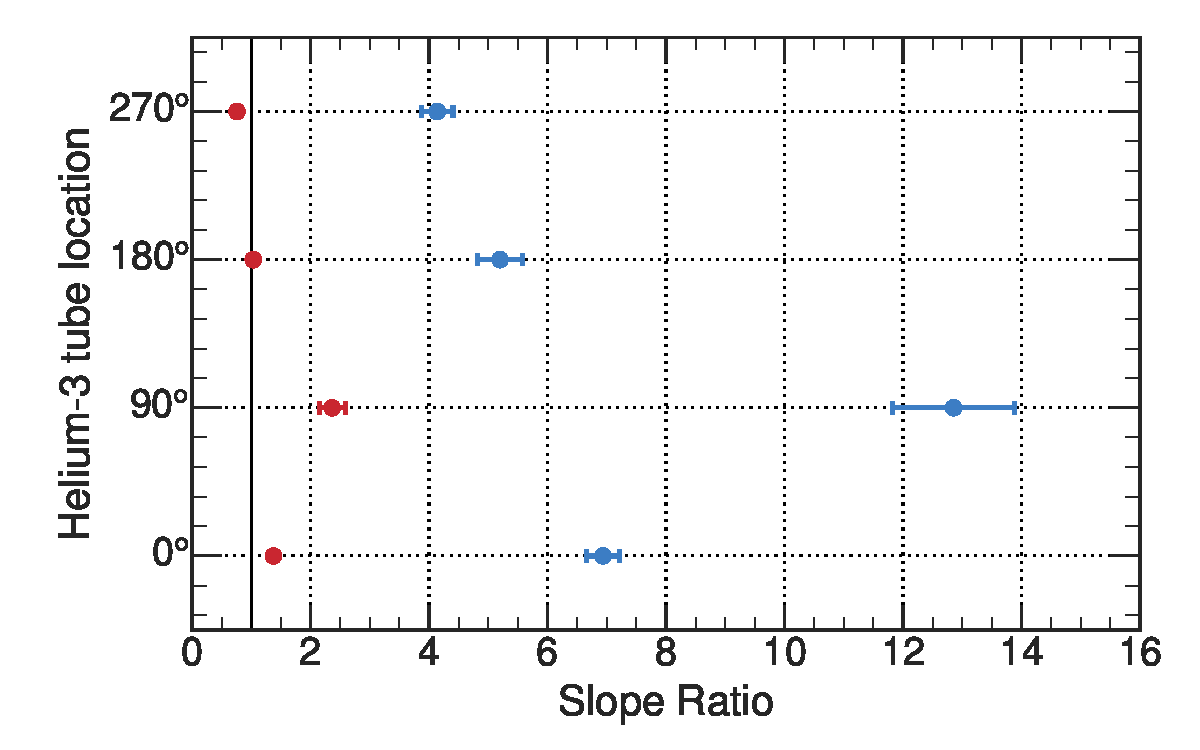
\includegraphics[width=\textwidth]{images/SlopeRatioPlot_He3}
	\caption[Comparison of gas models with slope ratio]{Comparison of gas models with slope ratio. Red is the ratio of the slopes from the $P\cdot I\cdot Z_{\mathrm{eff}}^2$ model and blue is ratio of the slopes from the $P\cdot I$ gas model. The black line is at a slope ratio of one.}	
	\label{fig:slopeRatio}
\end{figure}

As shown in the figure, including $Z_{\mathrm{eff}}$ in the gas model produces a significant improvement in understanding the response to the vacuum bump, indicating that a difference in the gas composition is mainly responsible for the different rate vs $P\cdot I$ dependence for the two bumps. This shows that the rate actually depends on $P\cdot I\cdot Z_{\mathrm{eff}}^2$. Note that the \he tubes at $\phi=0^{\circ}$ and 90$^{\circ}$ are not as close to 1 as 180$^{\circ}$ and 270$^{\circ}$, but are still much improved over the $P\cdot I$ model. Note that Fig~\ref{fig:rateVsPressCurWeight1} shows some systematic effect in the tube 1 (90$^{\circ}$) rates for the second bump, with a significant non-constant slope relative to the others, resulting in a much larger deviation in the slope ratio.


%------------------------------------------------------------------------------------------------



\section{Touschek experiments}
\label{sec:TousExp}

	In order to separate the beam-gas and beam-beam component of the \he tube rate during the beam size scans, the rate is fit to this function:
\begin{equation}
	{R_{^{3}\mathrm{He tube}} = c_{\mathrm{gas}}\cdot P\cdot I\cdot Z_{\mathrm{eff}}^{2}+c_{\mathrm{T}}\cdot \frac{I^{2}}{N_{\mathrm{Bunch}}\cdot\sigma_{y}}}
	\label{eqn:TousFit}
\end{equation}
where $P$ is the pressure in the beampipe, $I$ is the beam current, $Z_{\mathrm{eff}}$ is the atomic number of the beampipe gas, $\sigma_{y}$ is the size of the beam, and $c_{\mathrm{gas}}$ and $c_{\mathrm{T}}$ are the fit parameters. Fig~\ref{fig:tousZef} shows how $Z_{\mathrm{eff}}$ changes during the beam size runs, showing the importance of including it in the fit. For the LER, the value of $Z_{\mathrm{eff}}$ measured at D02 is used. This technique is described in detail in \S~\ref{sec:PBump}. The HER has no RGA, and therefore it is not possible to determine the value of $Z_{\mathrm{eff}}$, so a value of 1 is assumed. The $P_{\mathrm{scale}}$ factor used in the simulation scaling (see Chapter ~\ref{chap:Sim}) is 1.


\begin{figure}
	\centerfloat
		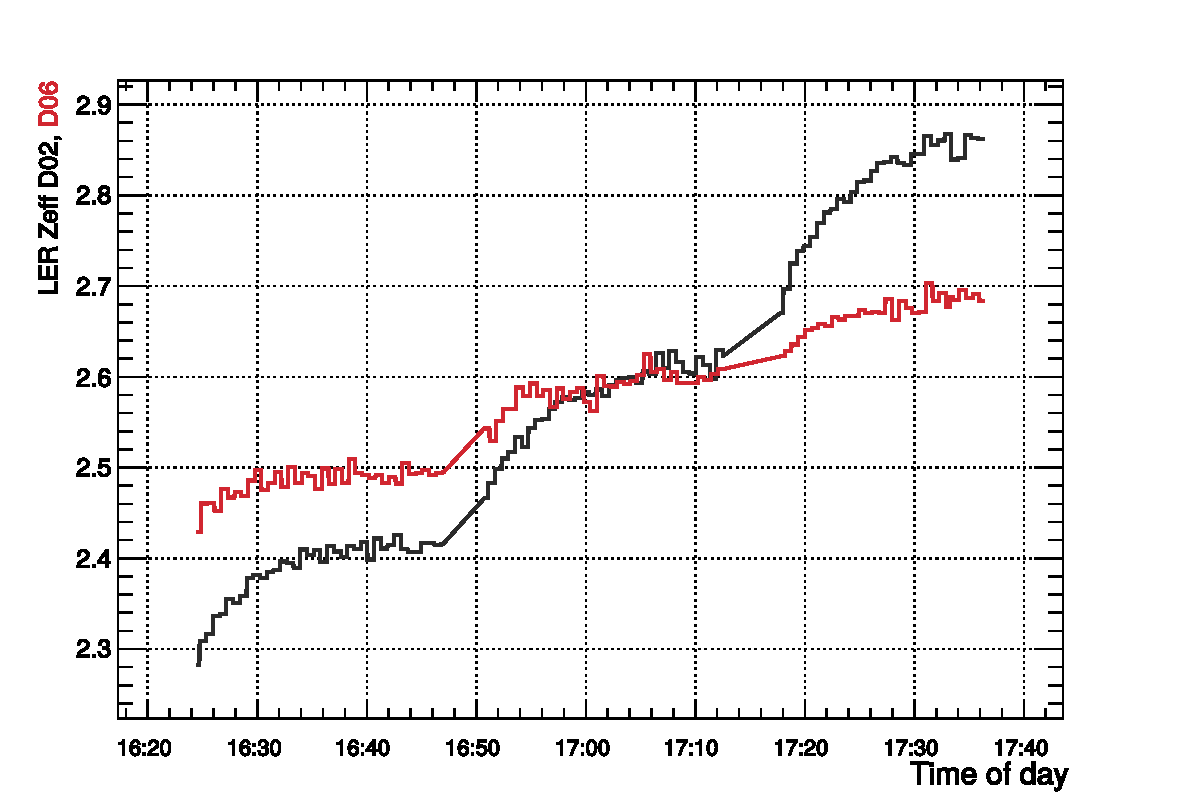
\includegraphics[width=\textwidth]{images/Zeff}
	\caption[$Z_{\mathrm{eff}}$ during LER beam size runs]{$Z_{\mathrm{eff}}$ during LER beam size runs. Data were recorded on May 17, 2016.}	
	\label{fig:tousZef}
\end{figure}

The results of this fit for data and simulation for LER and HER are shown in Figs~\ref{fig:LERTous10},~\ref{fig:LERTous11},~\ref{fig:LERTous12},~\ref{fig:LERTous13}, and~\ref{fig:HERTous10},~\ref{fig:HERTous11},~\ref{fig:HERTous12},~\ref{fig:HERTous13} respectively. The data are divided into three runs, each with five subruns. The runs occurred at different injection currents, and the subruns each had different beam sizes. In these figures, the black points are the average measured \he tube rate in each bin. The Touschek component, in green, is given by:
\begin{equation}
	R_{\mathrm{T}} = c_{\mathrm{T}}\cdot \frac{I^{2}}{N_{\mathrm{Bunch}}\cdot\sigma_{y}}
\end{equation}
and the beam-gas component, in blue, is given by:
\begin{equation}
	R_{\mathrm{gas}} = c_{\mathrm{gas}}\cdot P\cdot I\cdot Z_{\mathrm{eff}}^{2}
\end{equation}
The error bars shown are the RMS of the \he tube rate for that bin. The pressure in the beampipe is changing over the course of the experiments and is included in the fit, but for simplicity is not shown in the figures. The values produced by the fit can be found in Table~\ref{tab:FitPars}, and $\chi^2$ and number of degrees of freedom (ndf) are in Table~\ref{tab:ChiNDF}. Note that only statistical errors and fit parameters uncertainties are included in the $\chi^2$ calculation. If the systematic errors are included, $\chi^2$ becomes significantly smaller.


\begin{sidewaystable}
    \centering
    \begin{tabular}{cc|cc|cc|cccc}
	&		&	 \multicolumn{2}{c}{Data}			&	 \multicolumn{2}{c}{Simulation – Initial Scaling} 			&	 \multicolumn{2}{c}{Simulation – Corrected Scaling}  	 		\\	
	&	 	&	 c$_{\mathrm{gas}}$	&	 c$_{T}$	&	 c$_{\mathrm{gas}}$	&	 c$_{T}$ 	&	 c$_{\mathrm{gas}}$	&	 c$_{T}$ 	\\	
	&	Channel 	&	  [$Hz/(mA\cdot Pa)$]	&	 [$Hz\cdot\mu m/mA^{2}$]	&	 [$Hz/(mA\cdot Pa)$]	&	 [$Hz\cdot\mu m/mA^{2}$]  	&	  [$Hz/(mA\cdot Pa)$]	&	 [$Hz\cdot\mu m/mA^{2}$]  	\\	\hline \hline
LER	&	 0	&	 6500$\pm$400	&	 16.4$\pm$0.6	&	 3120.4$\pm$5	&	 8.028$\pm$0.007	&	 2963$\pm$5	&	 8.026$\pm$0.006	\\	
	&	 1	&	 3400$\pm$200	&	 8.1$\pm$0.3	&	 2401$\pm$4	&	 5.098$\pm$0.005	&	 2281$\pm$4	&	 5.097$\pm$0.005	\\	
	&	 2	&	 5700$\pm$300	&	 13.4$\pm$0.4	&	 1901$\pm$3	&	 4.653$\pm$0.004	&	 1806$\pm$3	&	 4.651$\pm$0.004	\\	
	&	 3	&	 8000$\pm$400	&	 18.1$\pm$0.5	&	 4076$\pm$7	&	 9.0245$\pm$0.008	&	 3872$\pm$7	&	 9.022$\pm$0.008	\\	\hline
HER	&	0	&	 (241$\pm$5)$\times10^{3}$	&	 0.21$\pm$0.04	&	 1750$\pm$30	&	 0.1963$\pm$0.0002 	&	 (151$\pm$1.5)$\times10^{3}$	&	 0.140$\pm$0.013	\\	
	&	1	&	 (108$\pm$4)$\times10^{3}$	&	 0.13$\pm$0.03	&	 1280.9$\pm$17	&	 0.0944$\pm$0.00014	&	 (104$\pm$1.0)$\times10^{3}$	&	 0.0507$\pm$0.009	\\	
	&	2	&	 (175$\pm$3)$\times10^{3}$	&	 0.21$\pm$0.03	&	 1030$\pm$15	&	 0.09052$\pm$0.00012	&	 (88.5$\pm$0.9)$\times10^{3}$ 	&	 0.0564$\pm$0.007	\\	
	&	3	&	 (241$\pm$4)$\times10^{3}$	&	 0.23$\pm$0.03	&	 2411$\pm$40	&	 0.26543$\pm$0.0003 	&	 (213$\pm$2.2)$\times10^{3}$	&	 0.189$\pm$0.018 	\\	\hline

    \end{tabular}
    \caption[Fit parameters associated with Figs~\ref{fig:LERTous10} to~\ref{fig:HERTous23}]{Fit parameters associated with Figs~\ref{fig:LERTous10} to~\ref{fig:HERTous23}. $\chi^2$ and ndf can be found in Table~\ref{tab:ChiNDF}.}
    \label{tab:FitPars}
\end{sidewaystable}


\begin{sidewaystable}
    \centering
    \begin{tabular}{cc|cc|cc|cccc}
	&		&	 \multicolumn{2}{c}{Data}			&	 \multicolumn{2}{c}{Simulation – Initial Scaling} 			&	 \multicolumn{2}{c}{Simulation – Corrected Scaling}  			\\	
	&	Channel 	&	$\chi^2$	&	ndf	&	$\chi^2$	&	ndf	&	$\chi^2$	&	ndf	\\	\hline \hline
LER	&	 0	&	141.57	&	12	&	23.206	&	12	&	21.504	&	12	\\	
	&	 1	&	85.587	&	12	&	30.489	&	12	&	28.446	&	12	\\	
	&	 2	&	106.37	&	12	&	24.988	&	12	&	23.192	&	12	\\	
	&	 3	&	116.51	&	12	&	28.789	&	12	&	26.819	&	12	\\	\hline
HER	&	0	&	7.7796	&	12	&	3.8825	&	12	&	24.408	&	12	\\	
	&	1	&	10.176	&	12	&	4.9767	&	12	&	22.25	&	12	\\	
	&	2	&	6.2589	&	12	&	4.333	&	12	&	21.303	&	12	\\	
	&	3	&	7.0256	&	12	&	3.8597	&	12	&	22.24	&	12	\\	\hline
    \end{tabular}
    \caption[$\chi^2$ and ndf for Figs~\ref{fig:LERTous10} to~\ref{fig:HERTous23}]{$\chi^2$ and ndf for Figs~\ref{fig:LERTous10} to~\ref{fig:HERTous23}. Note that only the statistical errors and fit parameter uncertainties are included in the calculation of $\chi^2$.}
    \label{tab:ChiNDF}
\end{sidewaystable}



\begin{figure}
	\centerfloat
		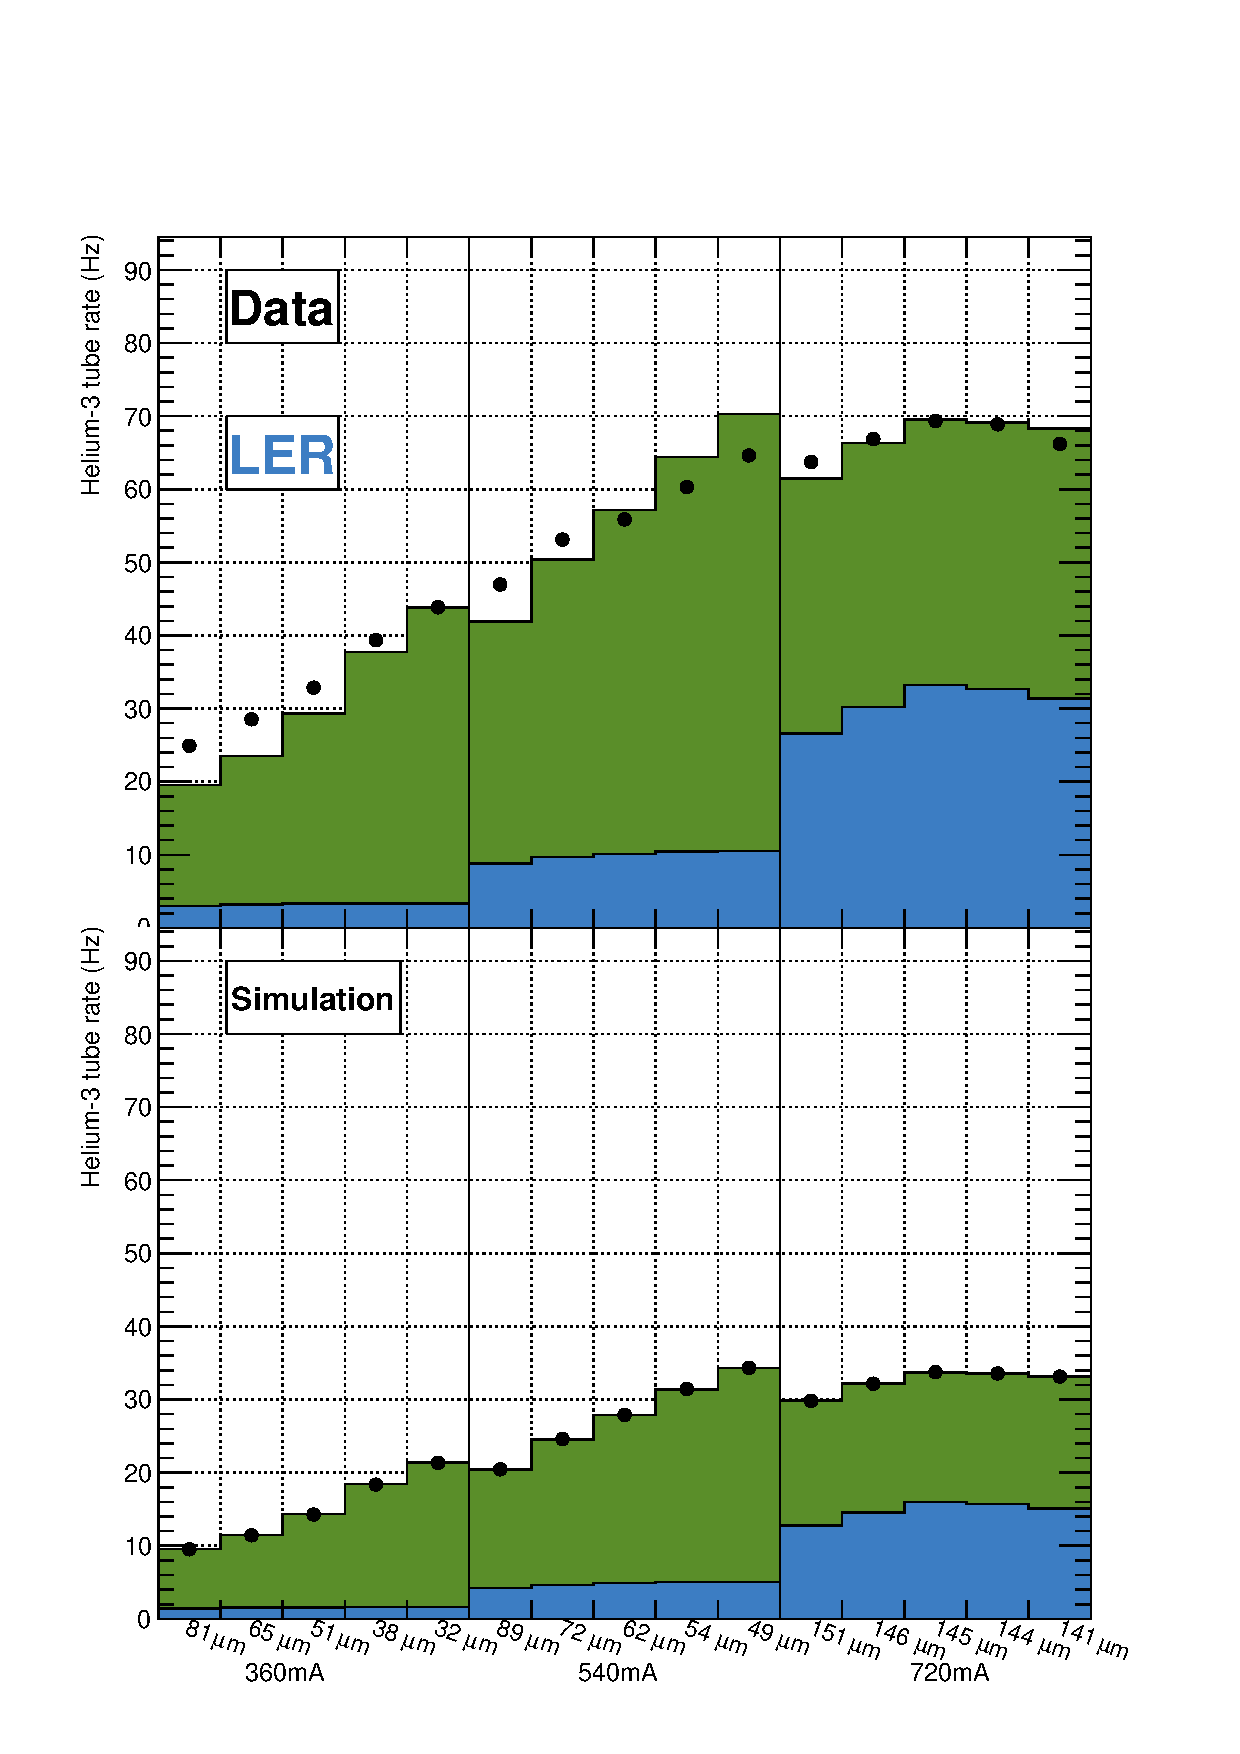
\includegraphics[width=\textwidth]{images/LERTousFirstPass_0}
		\begin{picture}(2,2)
			\put(-100,260){\thicklines\circle{10}} %1
			\put(-120,240){\thicklines\circle{10}}  %2
			\put(-100,220){\thicklines\circle{10}}  %3
			\put(-80,240){\thicklines\circle*{10}}   %0
			\put(-104, 237){$\phi$}  
		\end{picture}
	\caption[Result of fit for Touschek experiments, LER, channel 0]{Result of fit for Touschek experiments, LER, channel 0. Green is the beam-beam component, blue is the beam-gas component, and black is the rate measured in \he tube channel 0. Error bars are the standard deviation of the mean of the rate in that bin and are too small to be seen on this scale.}	
	\label{fig:LERTous10}
\end{figure}


\begin{figure}
	\centerfloat
		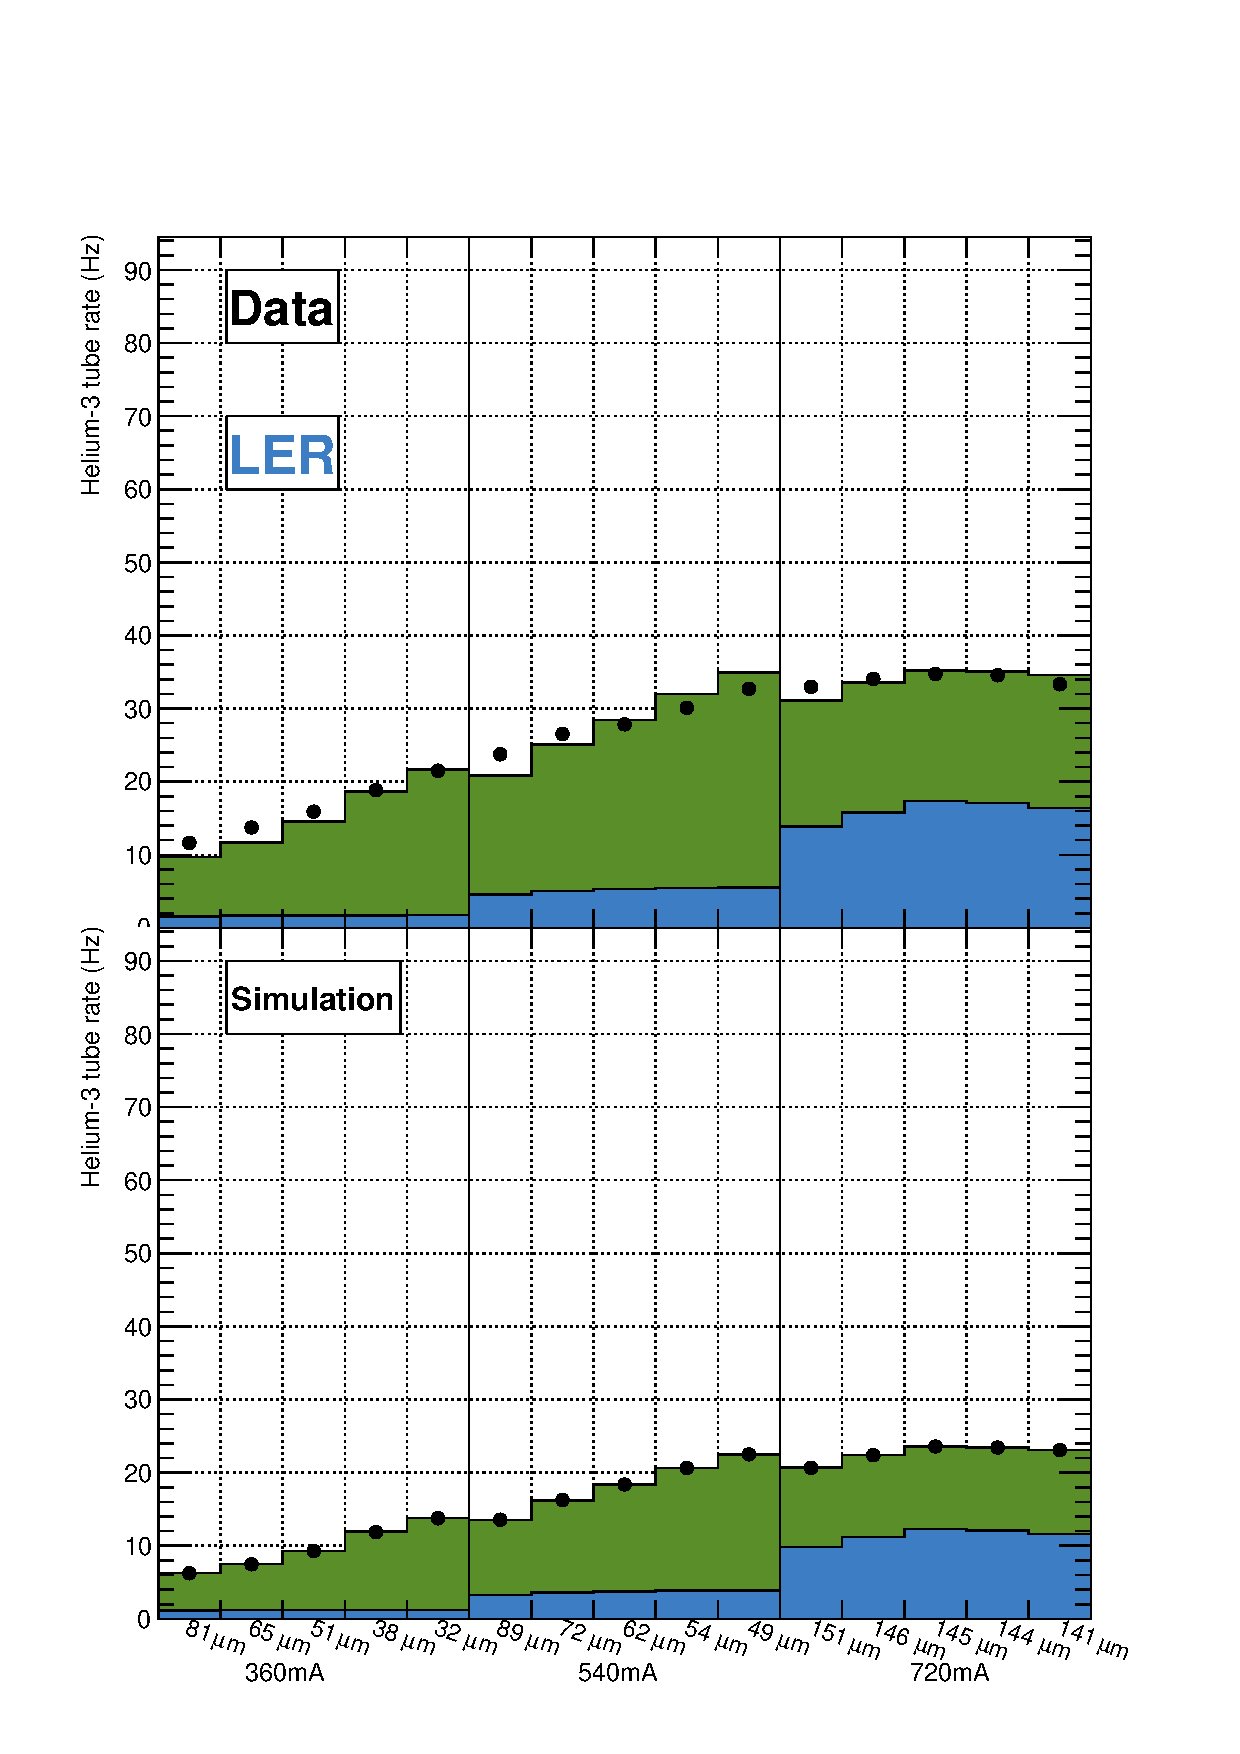
\includegraphics[width=\textwidth]{images/LERTousFirstPass_1}
		\begin{picture}(2,2)
			\put(-100,260){\thicklines\circle*{10}} %1
			\put(-120,240){\thicklines\circle{10}}  %2
			\put(-100,220){\thicklines\circle{10}}  %3
			\put(-80,240){\thicklines\circle{10}}   %0
			\put(-104, 237){$\phi$}  
		\end{picture}
	\caption[Result of fit for Touschek experiments, LER, channel 1]{Result of fit for Touschek experiments, LER, channel 1. Green is the beam-beam component, blue is the beam-gas component, and black is the rate measured in \he tube channel 1. Error bars are the standard deviation of the mean of the rate in that bin and are too small to be seen on this scale.}	
	\label{fig:LERTous11}
\end{figure}

\begin{figure}
	\centerfloat
		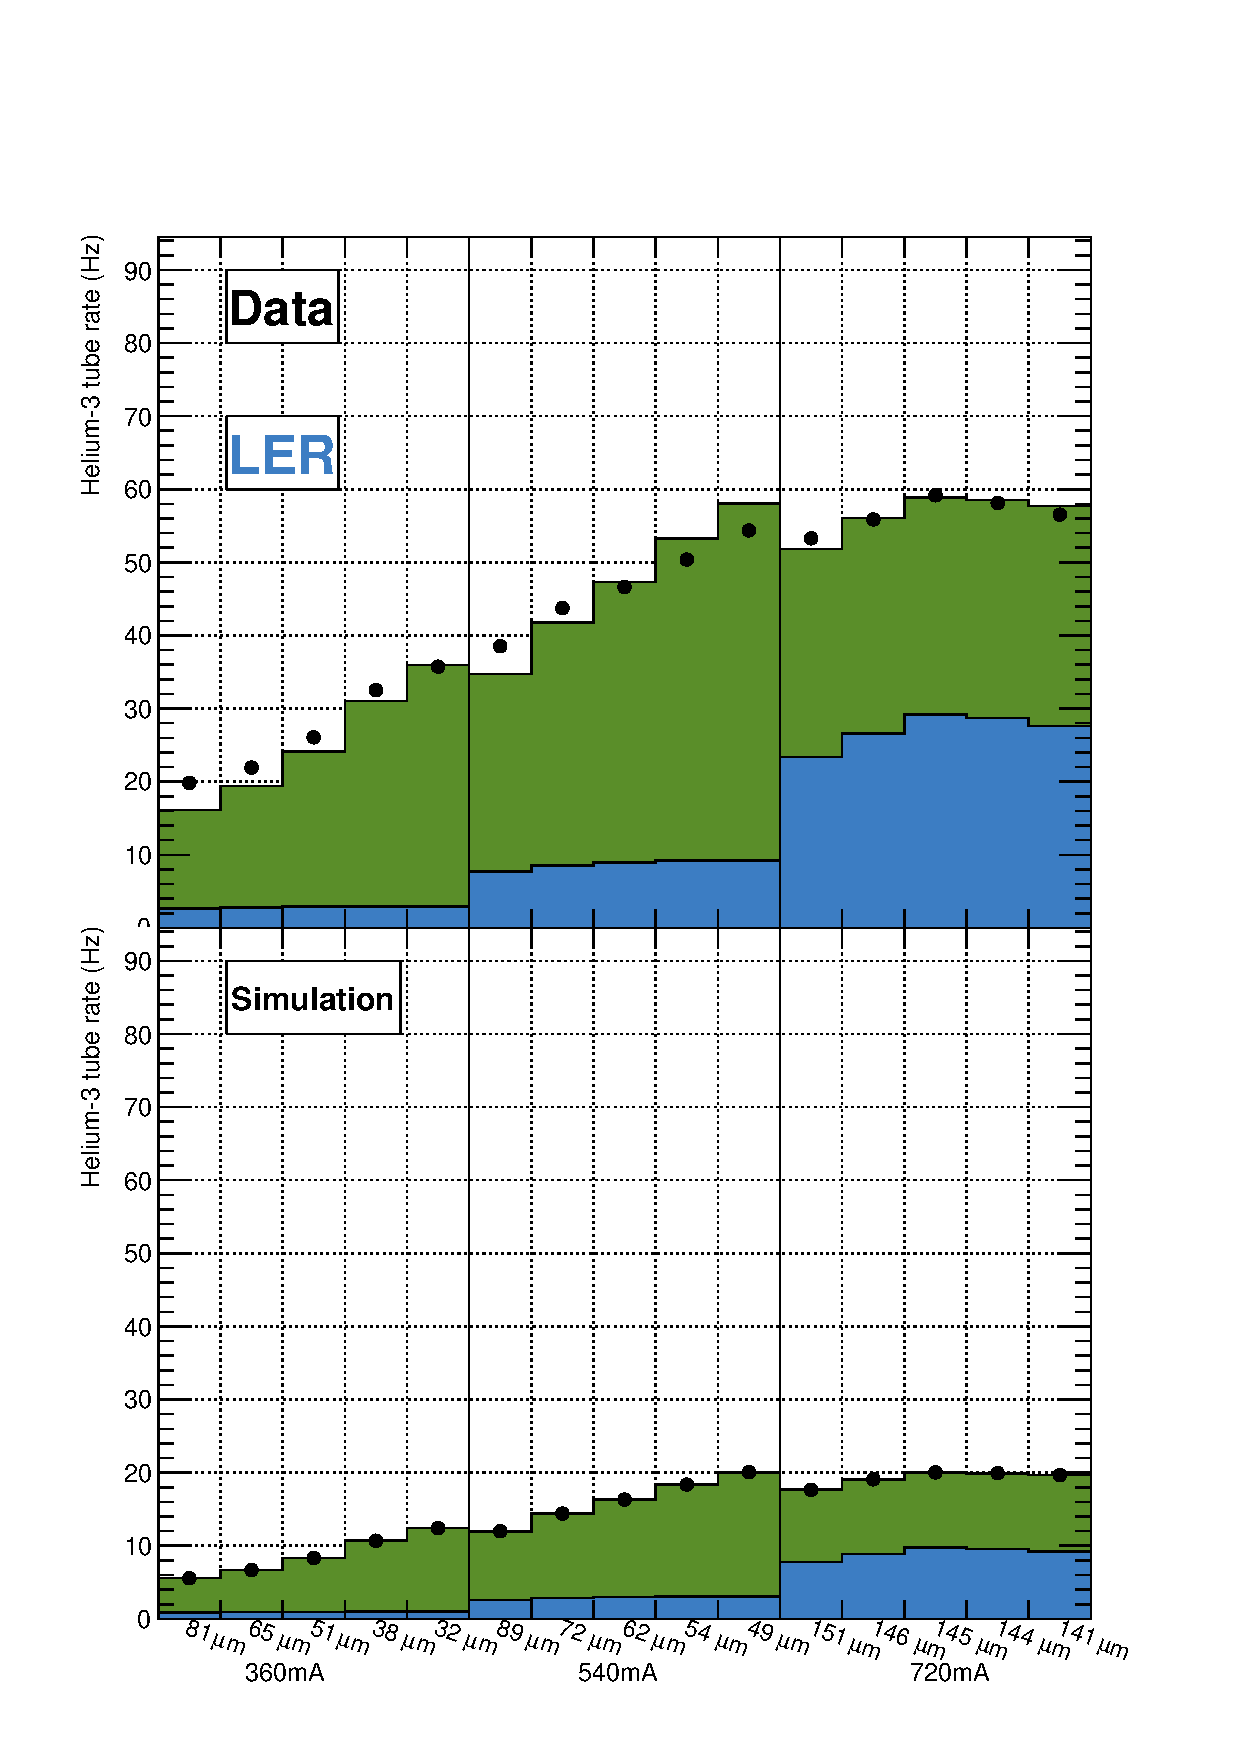
\includegraphics[width=\textwidth]{images/LERTousFirstPass_2}	
		\begin{picture}(2,2)
			\put(-100,260){\thicklines\circle{10}} %1
			\put(-120,240){\thicklines\circle*{10}}  %2
			\put(-100,220){\thicklines\circle{10}}  %3
			\put(-80,240){\thicklines\circle{10}}   %0
			\put(-104, 237){$\phi$}  
		\end{picture}
	\caption[Result of fit for Touschek experiments, LER, channel 2]{Result of fit for Touschek experiments, LER, channel 2. Green is the beam-beam component, blue is the beam-gas component, and black is the rate measured in \he tube channel 2. Error bars are the standard deviation of the mean of the rate in that bin and are too small to be seen on this scale.}	
	\label{fig:LERTous12}
\end{figure}

\begin{figure}
	\centerfloat
		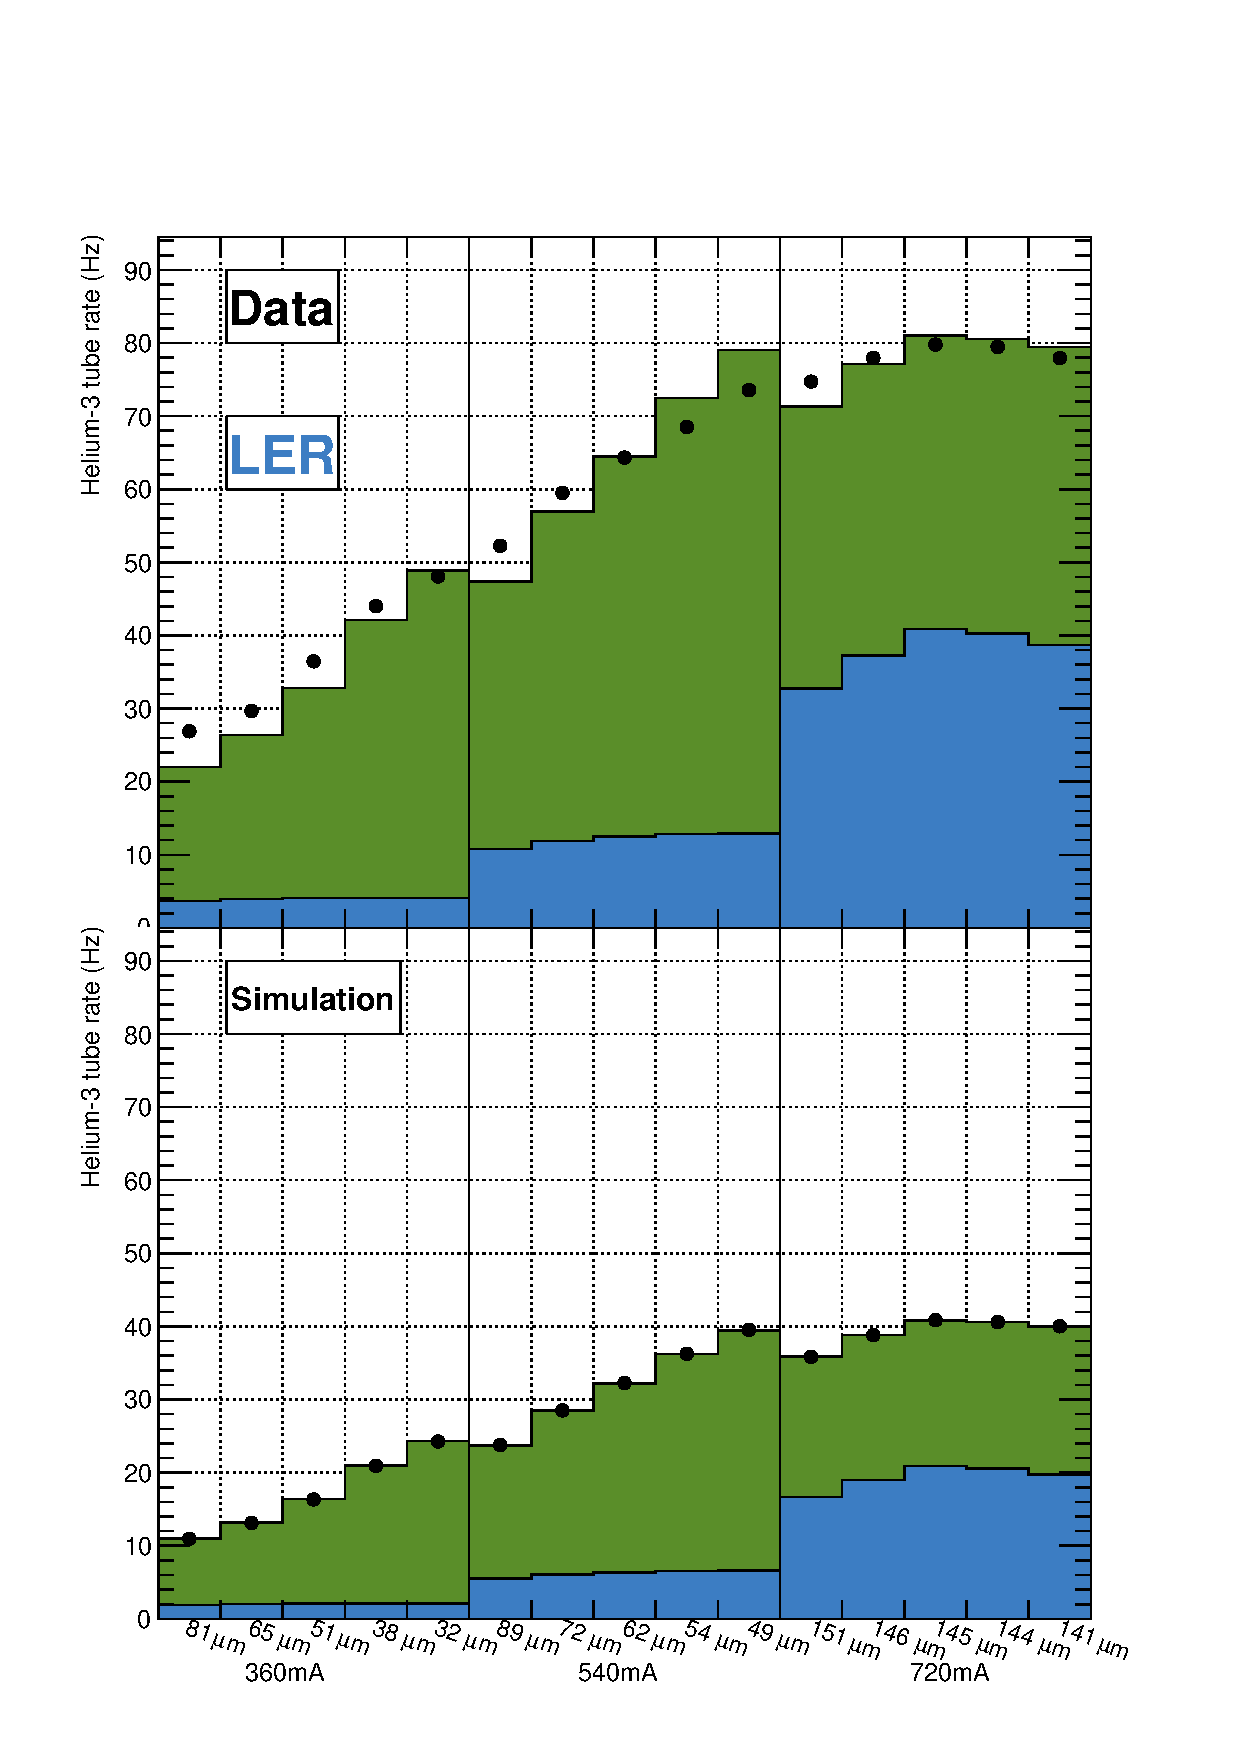
\includegraphics[width=\textwidth]{images/LERTousFirstPass_3}
		\begin{picture}(2,2)
			\put(-100,260){\thicklines\circle{10}} %1
			\put(-120,240){\thicklines\circle{10}}  %2
			\put(-100,220){\thicklines\circle*{10}}  %3
			\put(-80,240){\thicklines\circle{10}}   %0
			\put(-104, 237){$\phi$}  
		\end{picture}
	\caption[Result of fit for Touschek experiments, LER, channel 3]{Result of fit for Touschek experiments, LER, channel 3. Green is the beam-beam component, blue is the beam-gas component, and black is the rate measured in \he tube channel 3. Error bars are the standard deviation of the mean of the rate in that bin.}	
	\label{fig:LERTous13}
\end{figure}





\begin{figure}
	\centerfloat
		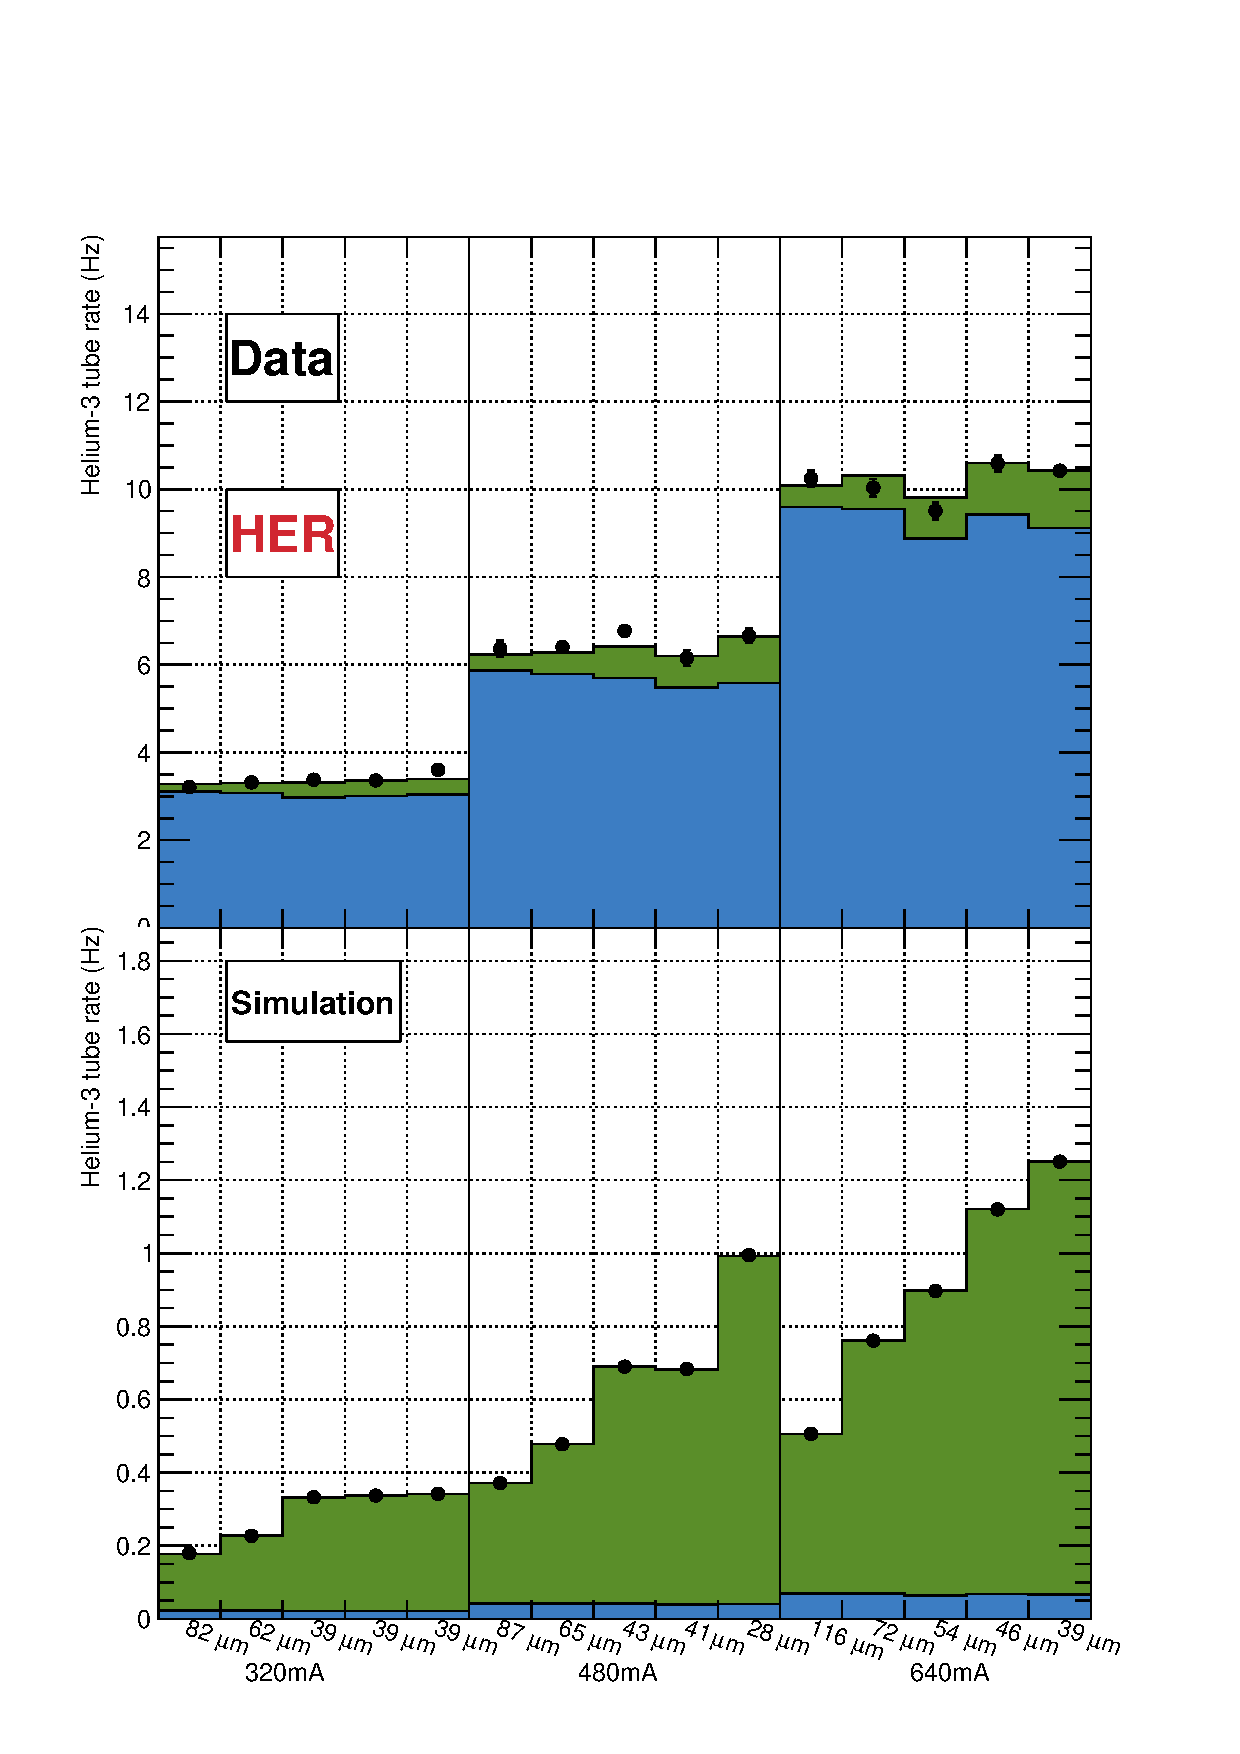
\includegraphics[width=\textwidth]{images/HERTousFirstPass_0}
		\begin{picture}(2,2)
			\put(-100,260){\thicklines\circle{10}} %1
			\put(-120,240){\thicklines\circle{10}}  %2
			\put(-100,220){\thicklines\circle{10}}  %3
			\put(-80,240){\thicklines\circle*{10}}   %0
			\put(-104, 237){$\phi$}  
		\end{picture}
	\caption[Result of fit for Touschek experiments, HER, channel 0]{Result of fit for Touschek experiments, HER, channel 0. Green is the beam-beam component, blue is the beam-gas component, and black is the rate measured in \he tube channel 0. Error bars are the standard deviation of the mean of the rate in that bin and are too small to be seen on this scale.}	
	\label{fig:HERTous10}
\end{figure}

\begin{figure}
	\centerfloat
		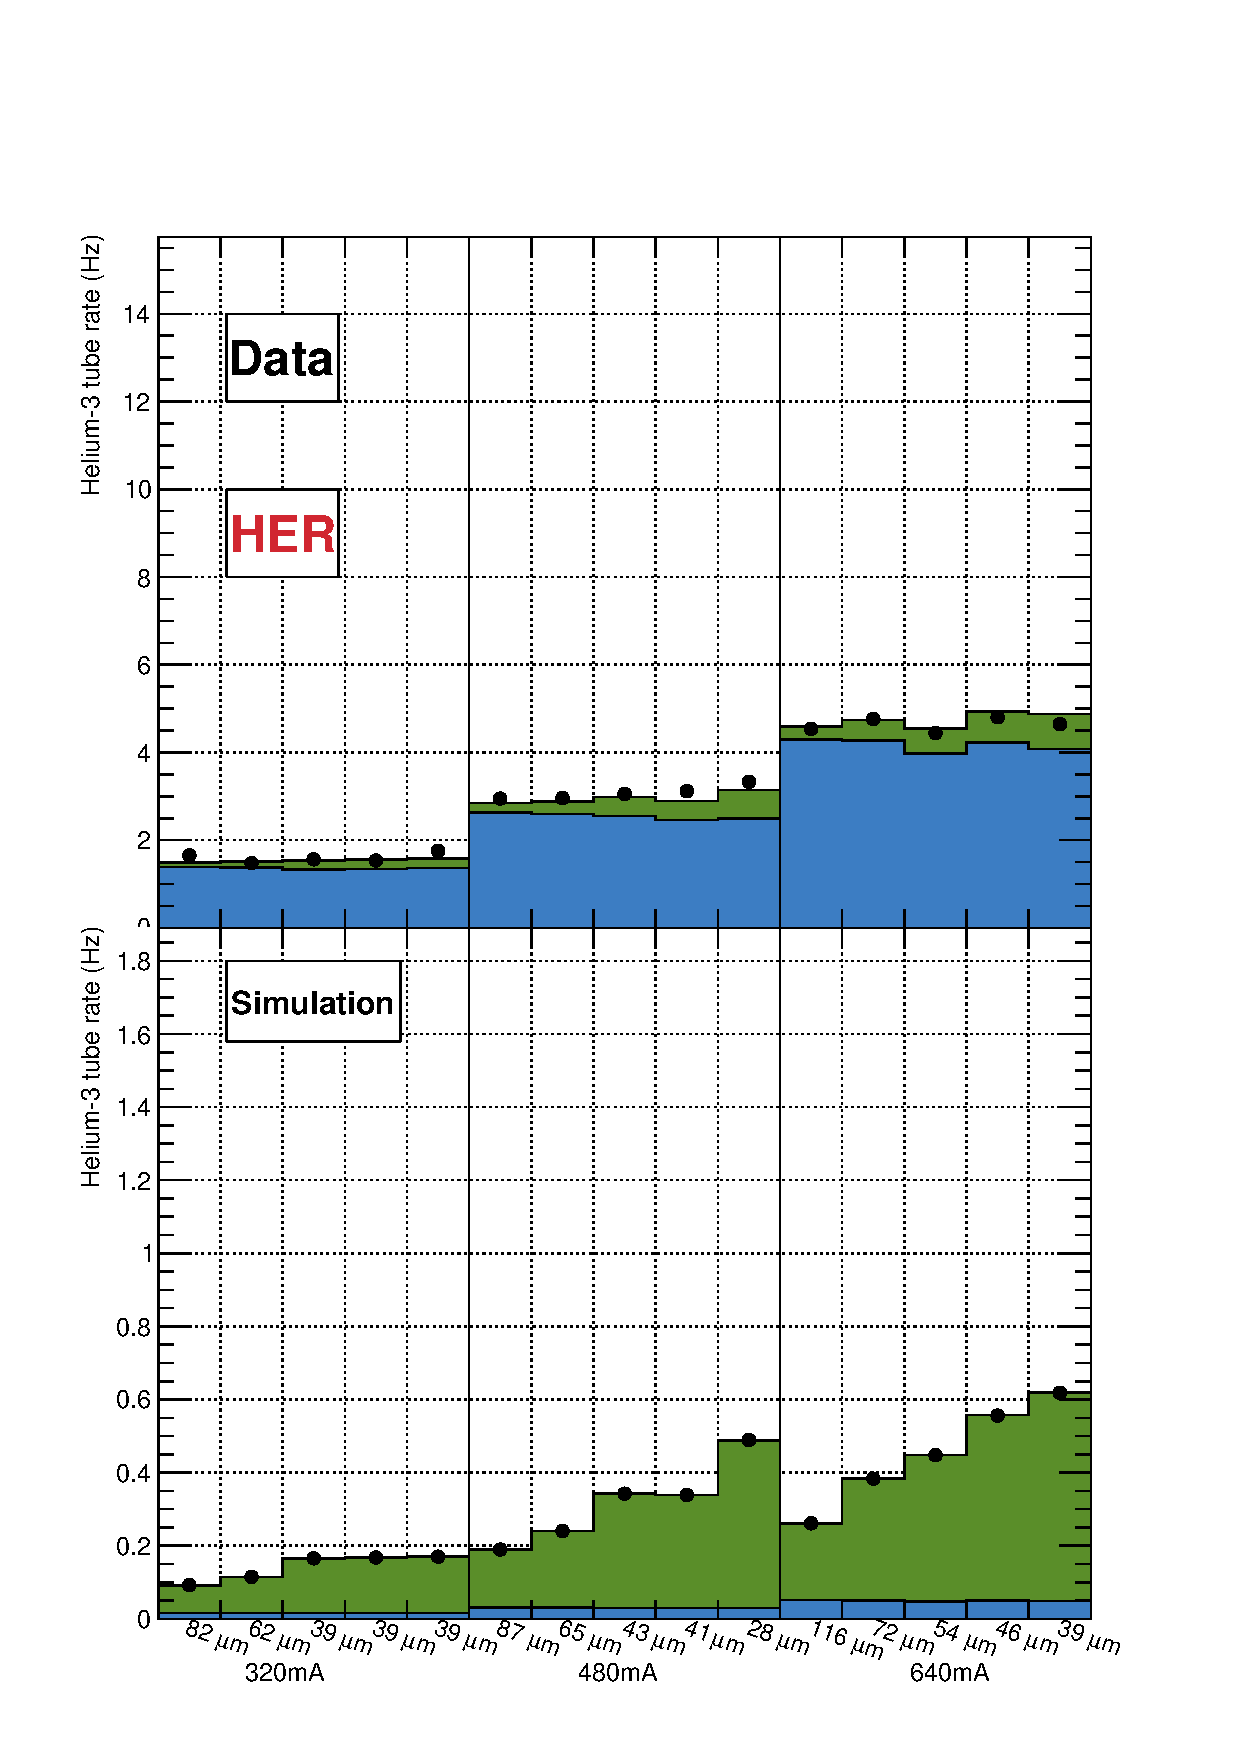
\includegraphics[width=\textwidth]{images/HERTousFirstPass_1}
		\begin{picture}(2,2)
			\put(-100,260){\thicklines\circle*{10}} %1
			\put(-120,240){\thicklines\circle{10}}  %2
			\put(-100,220){\thicklines\circle{10}}  %3
			\put(-80,240){\thicklines\circle{10}}   %0
			\put(-104, 237){$\phi$}  
		\end{picture}
	\caption[Result of fit for Touschek experiments, HER, channel 1]{Result of fit for Touschek experiments, HER, channel 1. Green is the beam-beam component, blue is the beam-gas component, and black is the rate measured in \he tube channel 1. Error bars are the standard deviation of the mean of the rate in that bin and are too small to be seen on this scale.}	
	\label{fig:HERTous11}
\end{figure}
\begin{figure}
	\centerfloat
		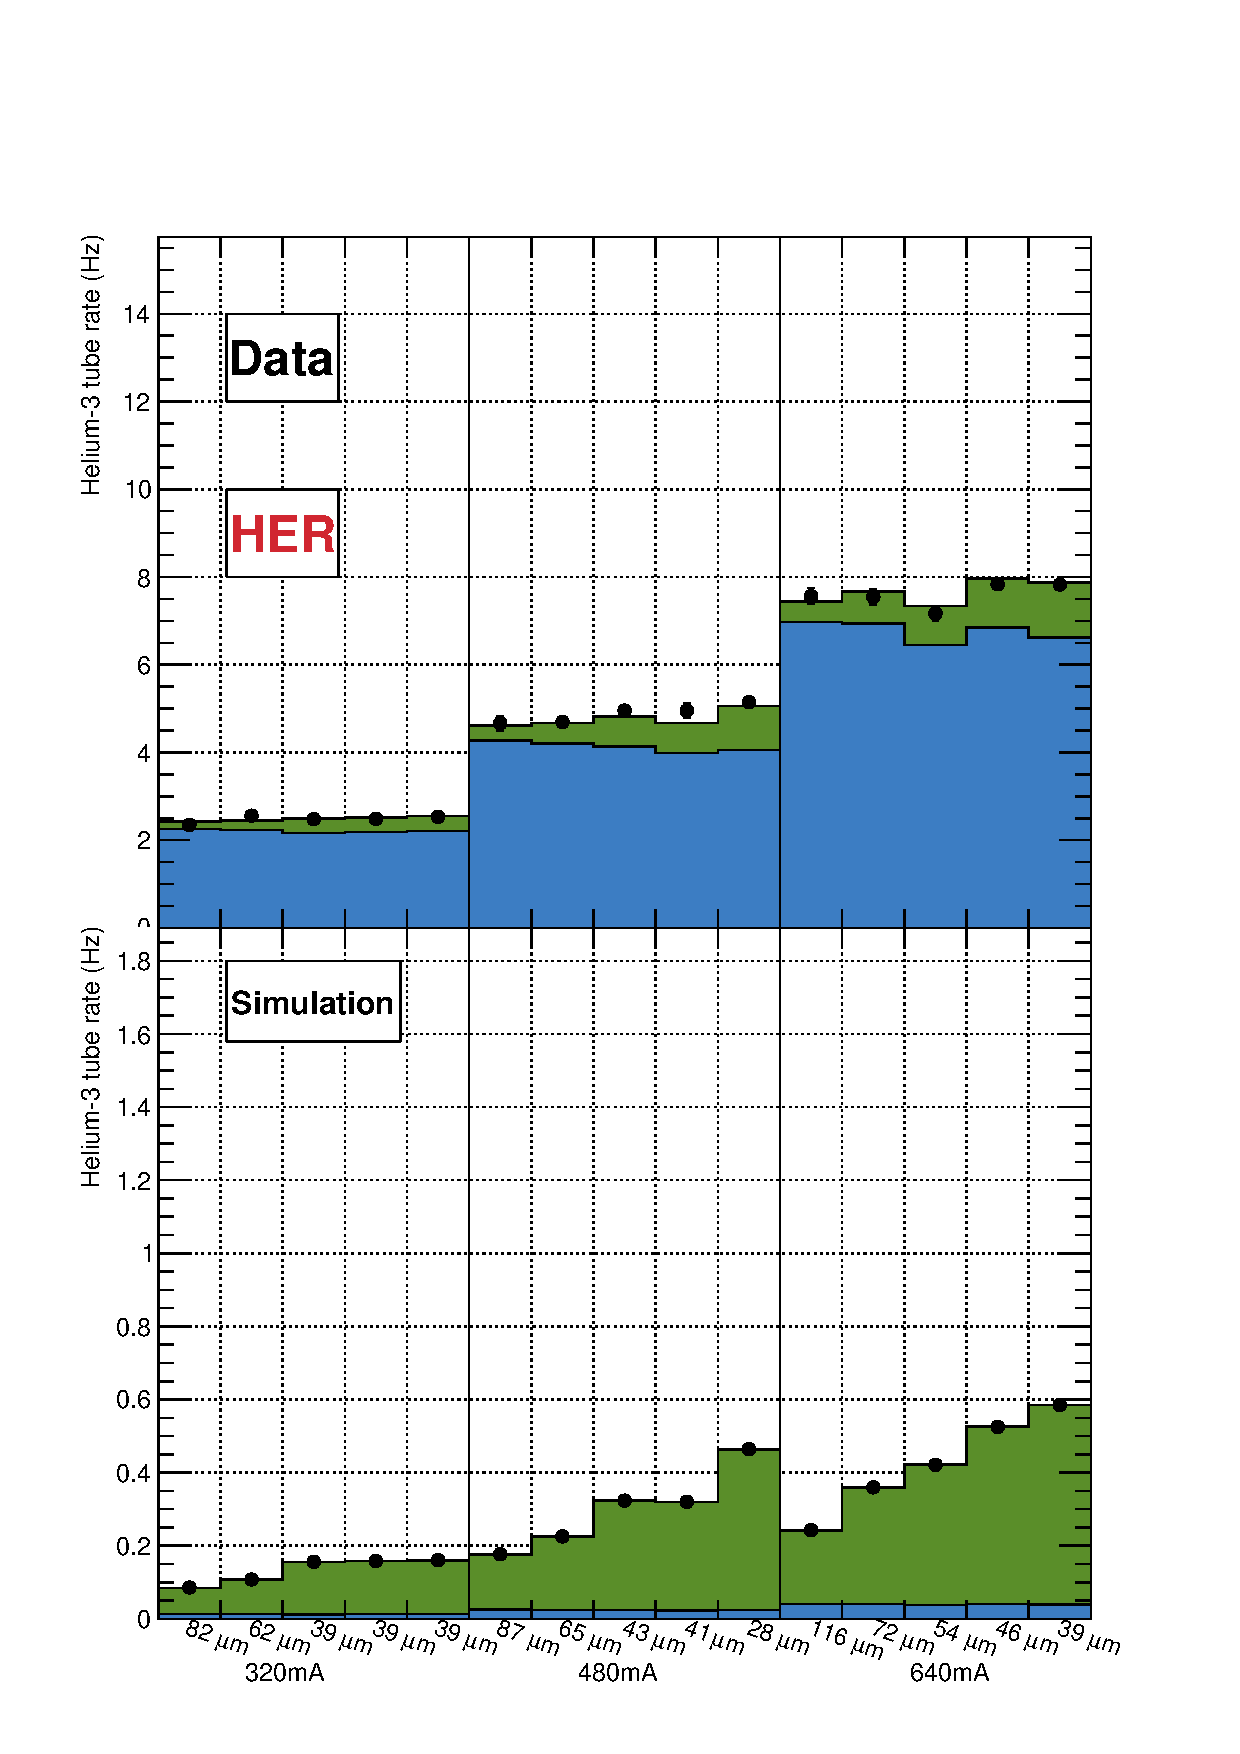
\includegraphics[width=\textwidth]{images/HERTousFirstPass_2}
		\begin{picture}(2,2)
			\put(-100,260){\thicklines\circle{10}} %1
			\put(-120,240){\thicklines\circle*{10}}  %2
			\put(-100,220){\thicklines\circle{10}}  %3
			\put(-80,240){\thicklines\circle{10}}   %0
			\put(-104, 237){$\phi$}  
		\end{picture}
	\caption[Result of fit for Touschek experiments, HER, channel 2]{Result of fit for Touschek experiments, HER, channel 2. Green is the beam-beam component, blue is the beam-gas component, and black is the rate measured in \he tube channel 2. Error bars are the standard deviation of the mean of the rate in that bin and are too small to be seen on this scale.}	
	\label{fig:HERTous12}
\end{figure}
\begin{figure}
	\centerfloat
		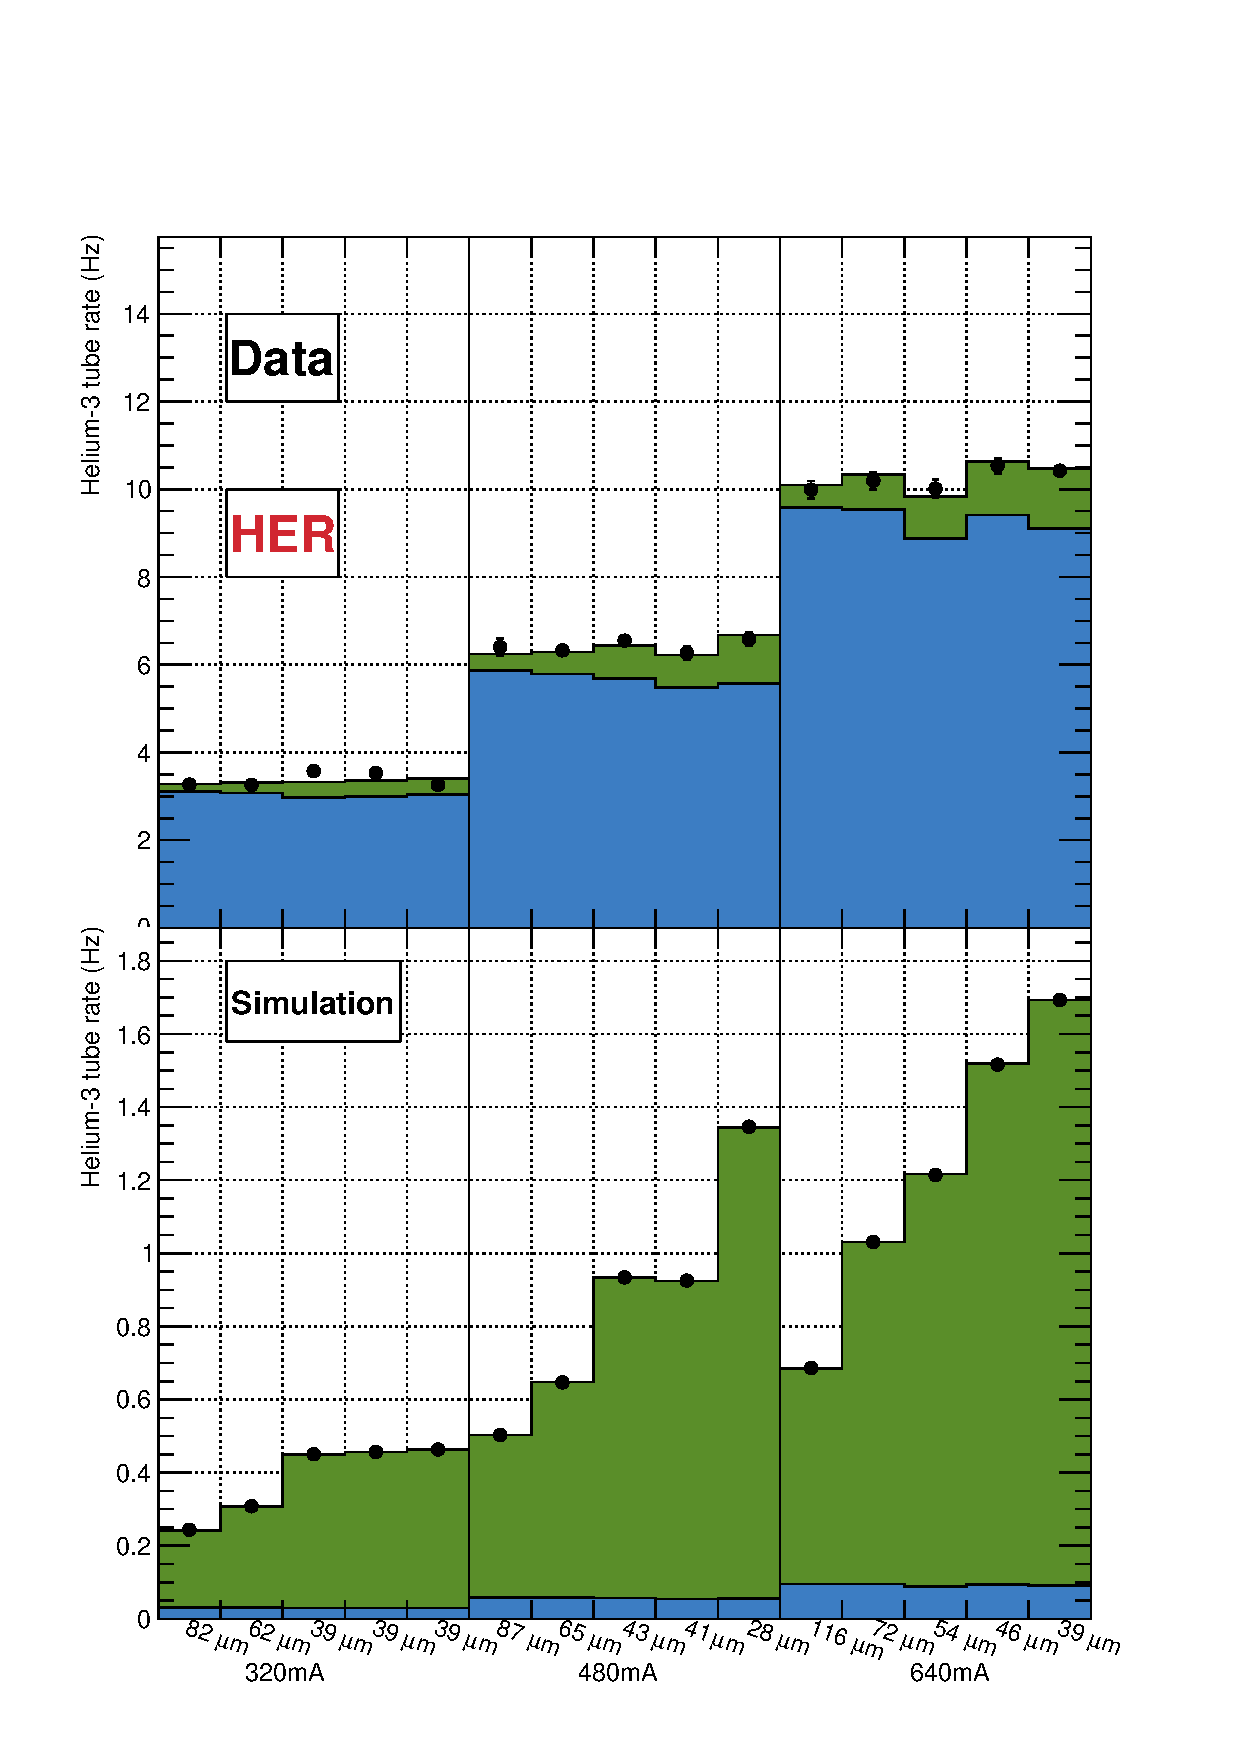
\includegraphics[width=\textwidth]{images/HERTousFirstPass_3}
		\begin{picture}(2,2)
			\put(-100,260){\thicklines\circle{10}} %1
			\put(-120,240){\thicklines\circle{10}}  %2
			\put(-100,220){\thicklines\circle*{10}}  %3
			\put(-80,240){\thicklines\circle{10}}   %0
			\put(-104, 237){$\phi$}  
		\end{picture}
	\caption[Result of fit for Touschek experiments, HER, channel 3]{Result of fit for Touschek experiments, HER, channel 3. Green is the beam-beam component, blue is the beam-gas component, and black is the rate measured in \he tube channel 3. Error bars are the standard deviation of the mean of the rate in that bin and are too small to be seen on this scale.}	
	\label{fig:HERTous13}
\end{figure}





As evident from Figs~\ref{fig:HERTous10} -~\ref{fig:HERTous13}, the simulation greatly underestimates the beam-gas component in the HER, and to a lesser extent in the LER. This is due to two factors: $Z_{\mathrm{eff}}$ is not known in the HER, and $P_{\mathrm{scale}}$ is not known in either beam. Using a value of 1 for these parameters does not give the correct beam-gas component. To compensate, the ratio of the beam-gas fit parameter, $c_{gas}$, to the Touschek fit parameter, $c_{T}$, for data is used to estimate a value for $P_{\mathrm{scale}}Z_{\mathrm{eff}}^{2}$ (or simply $P_{\mathrm{scale}}$ for the LER, since $Z$ is known) that is used in the weighting of the simulation:
\begin{equation}
	{P_{\mathrm{scale}}Z_{\mathrm{eff}}^{2} = \frac{\sum_{n=1}^{4}(c_{\mathrm{gas}}/c_{\mathrm{T}})_{i~\mathrm{data}}}{\sum_{n=1}^{4}(c_{\mathrm{gas}}/c_{\mathrm{T}})_{i~\mathrm{sim}}}}
\label{eqn:Pscale1}
\end{equation}
The motivation for this is that all the parameters of the Touschek component of the fit are relatively well known, while the pressure and $Z_{\mathrm{eff}}$ in the beam-gas component are not well known. The beam-gas to Touschek ratio in the data is used to determine $P_{\mathrm{scale}}Z_{\mathrm{eff}}^{2}$ to be used in the simulation weighting. Note that this does not constrain the overall total prediction of the background from the simulation or the absolute individual contributions.

\begin{table}[htb]
	\centering
	\begin{tabular}{ ccS }
	& $P_{\mathrm{scale}}$ (LER)	&	{$P_{\mathrm{scale}}Z_{\mathrm{eff}}^{2}$ (HER)}	\\	\hline \hline
0	&	0.980	&	122.07	\\	
1	&	0.853	&	73.45	\\	
2	&	1.019	&	88.62	\\	
3	&	0.962	&	115.10	\\	\hline
Combined (see Eqn~\ref{eqn:Pscale1})	&	0.950	&	96.27	\\	\hline

	\end{tabular}	
	\caption[$P_{\mathrm{scale}}$ and $P_{\mathrm{scale}}Z_{\mathrm{eff}}^{2}$ values]{$P_{\mathrm{scale}}$ and $P_{\mathrm{scale}}Z_{\mathrm{eff}}^{2}$ values.}
	\label{tab:PScaleZsq}
\end{table}

The values for $P_{\mathrm{scale}}Z_{\mathrm{eff}}^{2}$ can be found in Table~\ref{tab:PScaleZsq}. Note that the values are significantly different between LER and HER. This is because the $Z_{\mathrm{eff}}$ is known for the LER, but not the HER. 

The simulation was then re-weighted, and the data and simulation were again fit to Eqn~\ref{eqn:TousFit}. The results of the fit for LER and HER are shown in Figs~\ref{fig:LERTous20},~\ref{fig:LERTous21},~\ref{fig:LERTous22},~\ref{fig:LERTous23} and~\ref{fig:HERTous20},~\ref{fig:HERTous21},~\ref{fig:HERTous22},~\ref{fig:HERTous23}, respectively. The values of the fit parameters can be found in Table~\ref{tab:FitPars}.



\begin{figure}
	\centerfloat
		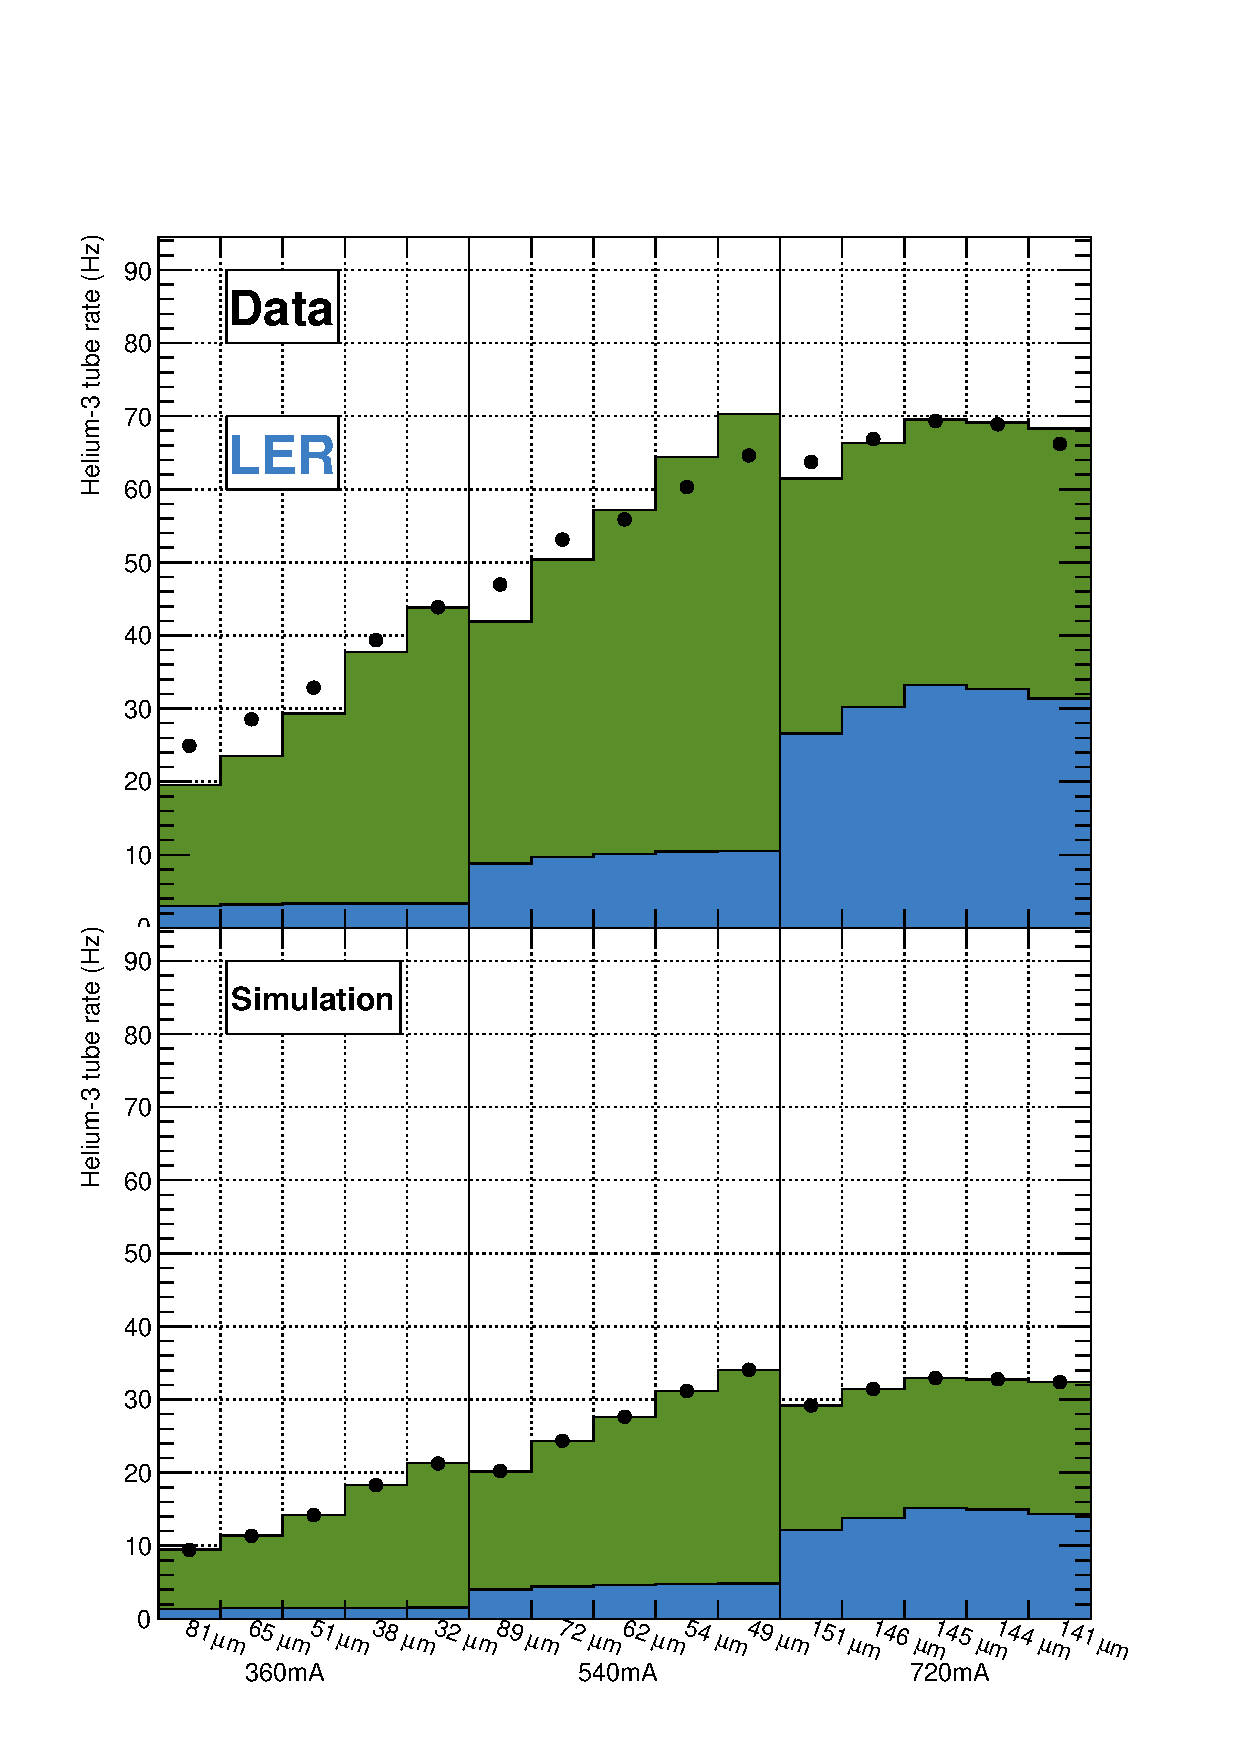
\includegraphics[width=\textwidth]{images/LERTousSecondPass_0}
		\begin{picture}(2,2)
			\put(-100,260){\thicklines\circle{10}}
			\put(-120,240){\thicklines\circle{10}}
			\put(-100,220){\thicklines\circle{10}}
			\put(-80,240){\thicklines\circle*{10}}
			\put(-104, 237){$\phi$}  
		\end{picture}
	\caption[Result of fit for Touschek experiments after simulation is weighted by $P_{\mathrm{scale}}$, LER, channel 0]{Result of fit for Touschek experiments after simulation is weighted by $P_{\mathrm{scale}}$, LER, channel 0. Green is the beam-beam component, blue is the beam-gas component, and black is the rate measured in \he tube channel 0. Error bars are the standard deviation of the mean of the rate in that bin and are too small to be seen on this scale.}	
	\label{fig:LERTous20}
\end{figure}

\begin{figure}
	\centerfloat
		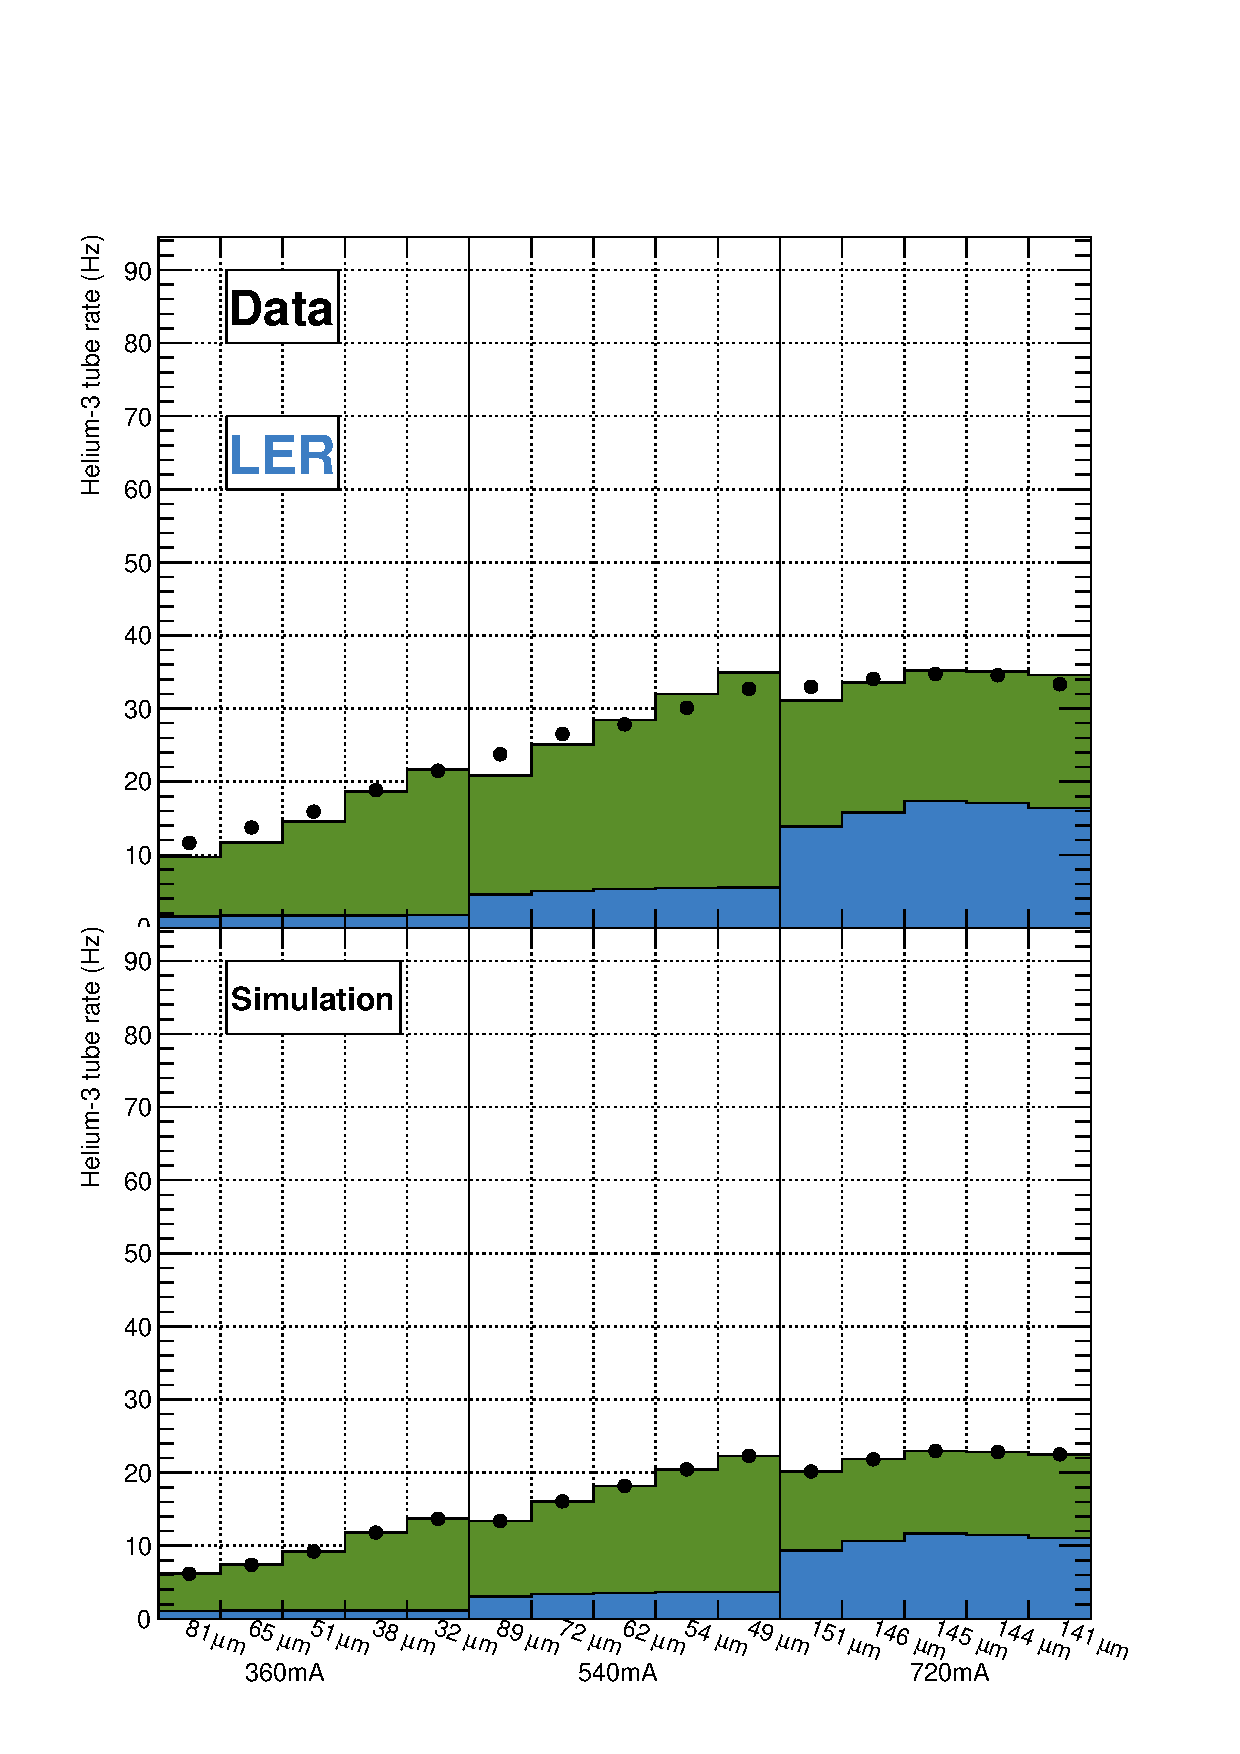
\includegraphics[width=\textwidth]{images/LERTousSecondPass_1}
		\begin{picture}(2,2)
			\put(-100,260){\thicklines\circle*{10}}
			\put(-120,240){\thicklines\circle{10}}
			\put(-100,220){\thicklines\circle{10}}
			\put(-80,240){\thicklines\circle{10}}
			\put(-104, 237){$\phi$}  
		\end{picture}
	\caption[Result of fit for Touschek experiments after simulation is weighted by $P_{\mathrm{scale}}$, LER, channel 1]{Result of fit for Touschek experiments after simulation is weighted by $P_{\mathrm{scale}}$, LER, channel 1. Green is the beam-beam component, blue is the beam-gas component, and black is the rate measured in \he tube channel 1. Error bars are the standard deviation of the mean of the rate in that bin and are too small to be seen on this scale.}	
	\label{fig:LERTous21}
\end{figure}

\begin{figure}
	\centerfloat
		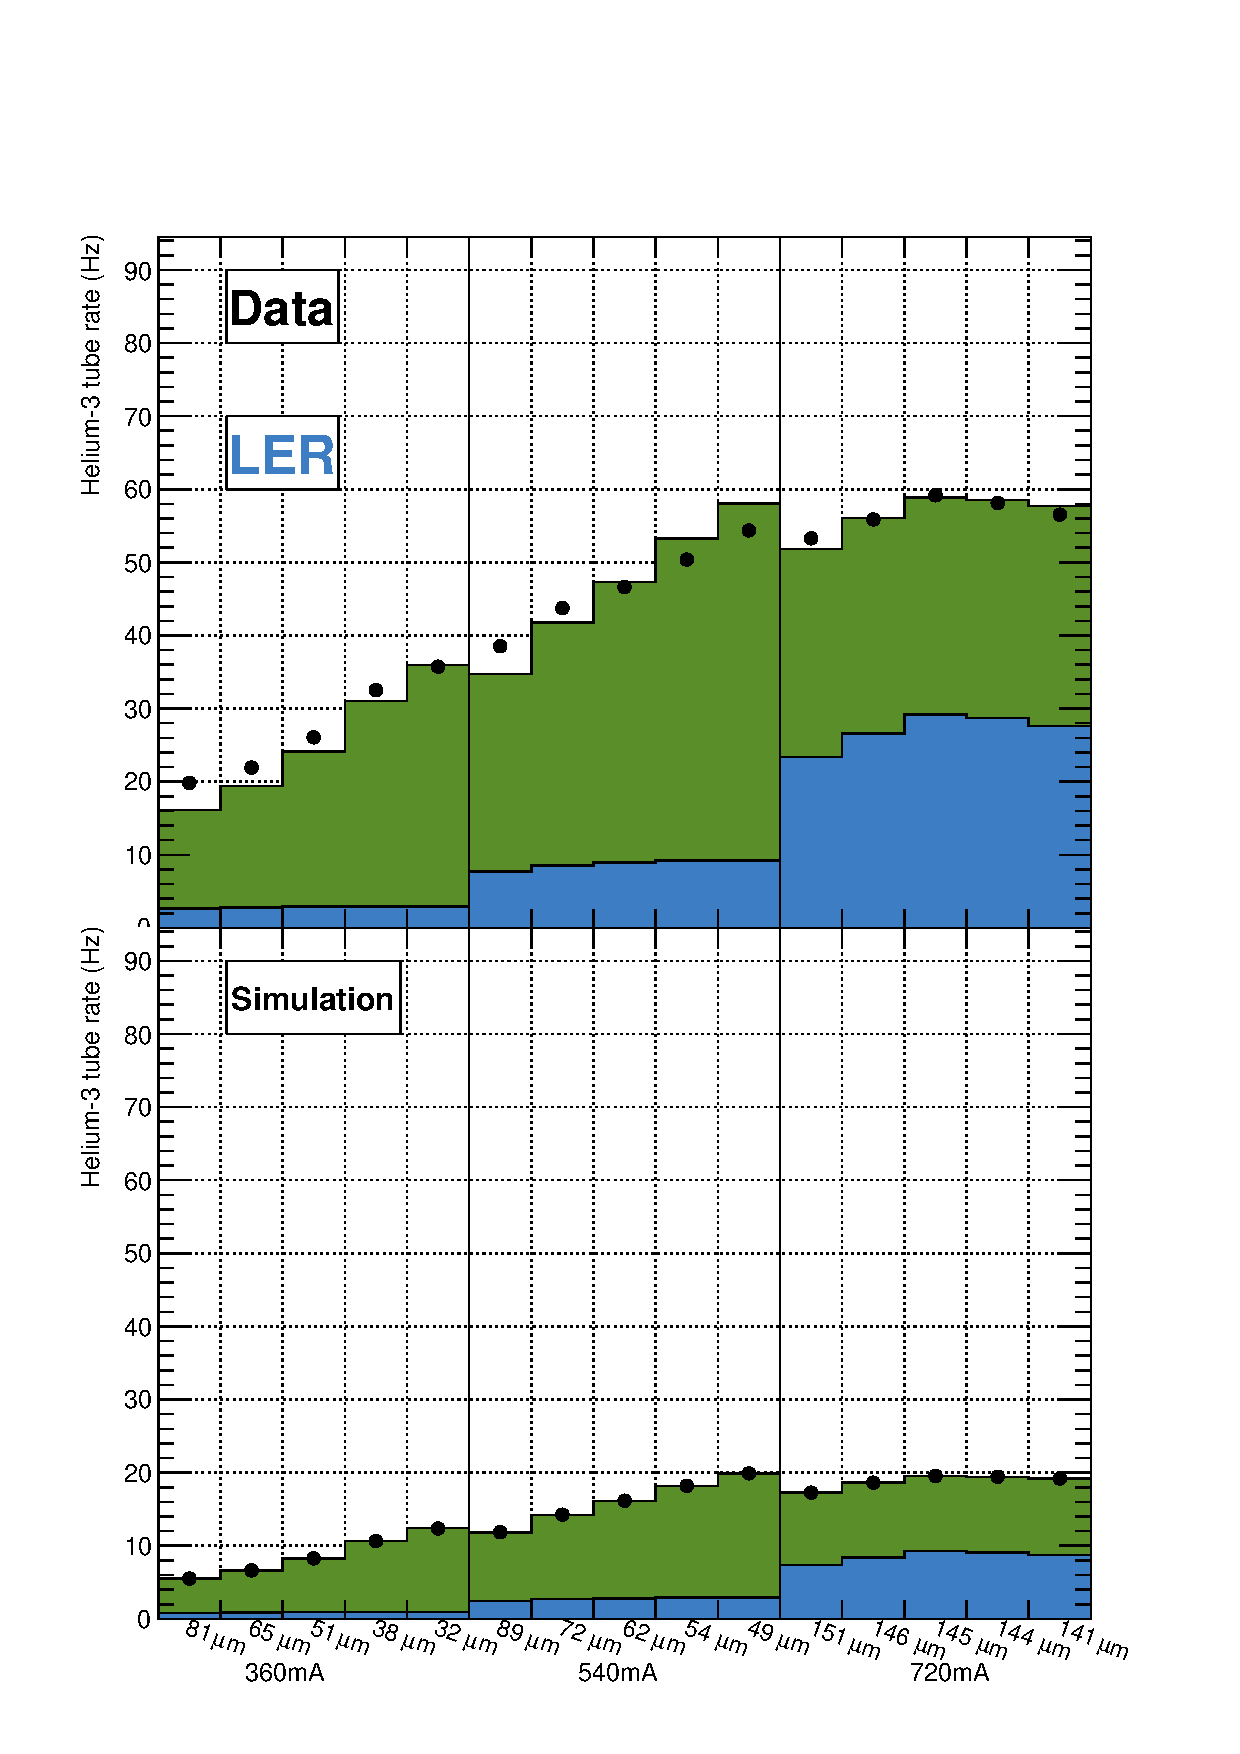
\includegraphics[width=\textwidth]{images/LERTousSecondPass_2}
		\begin{picture}(2,2)
			\put(-100,260){\thicklines\circle{10}}
			\put(-120,240){\thicklines\circle*{10}}
			\put(-100,220){\thicklines\circle{10}}
			\put(-80,240){\thicklines\circle{10}}
			\put(-104, 237){$\phi$}  
		\end{picture}
	\caption[Result of fit for Touschek experiments after simulation is weighted by $P_{\mathrm{scale}}$, LER, channel 2]{Result of fit for Touschek experiments after simulation is weighted by $P_{\mathrm{scale}}$, LER, channel 2. Green is the beam-beam component, blue is the beam-gas component, and black is the rate measured in \he tube channel 2. Error bars are the standard deviation of the mean of the rate in that bin and are too small to be seen on this scale.}	
	\label{fig:LERTous22}
\end{figure}

\begin{figure}
	\centerfloat
		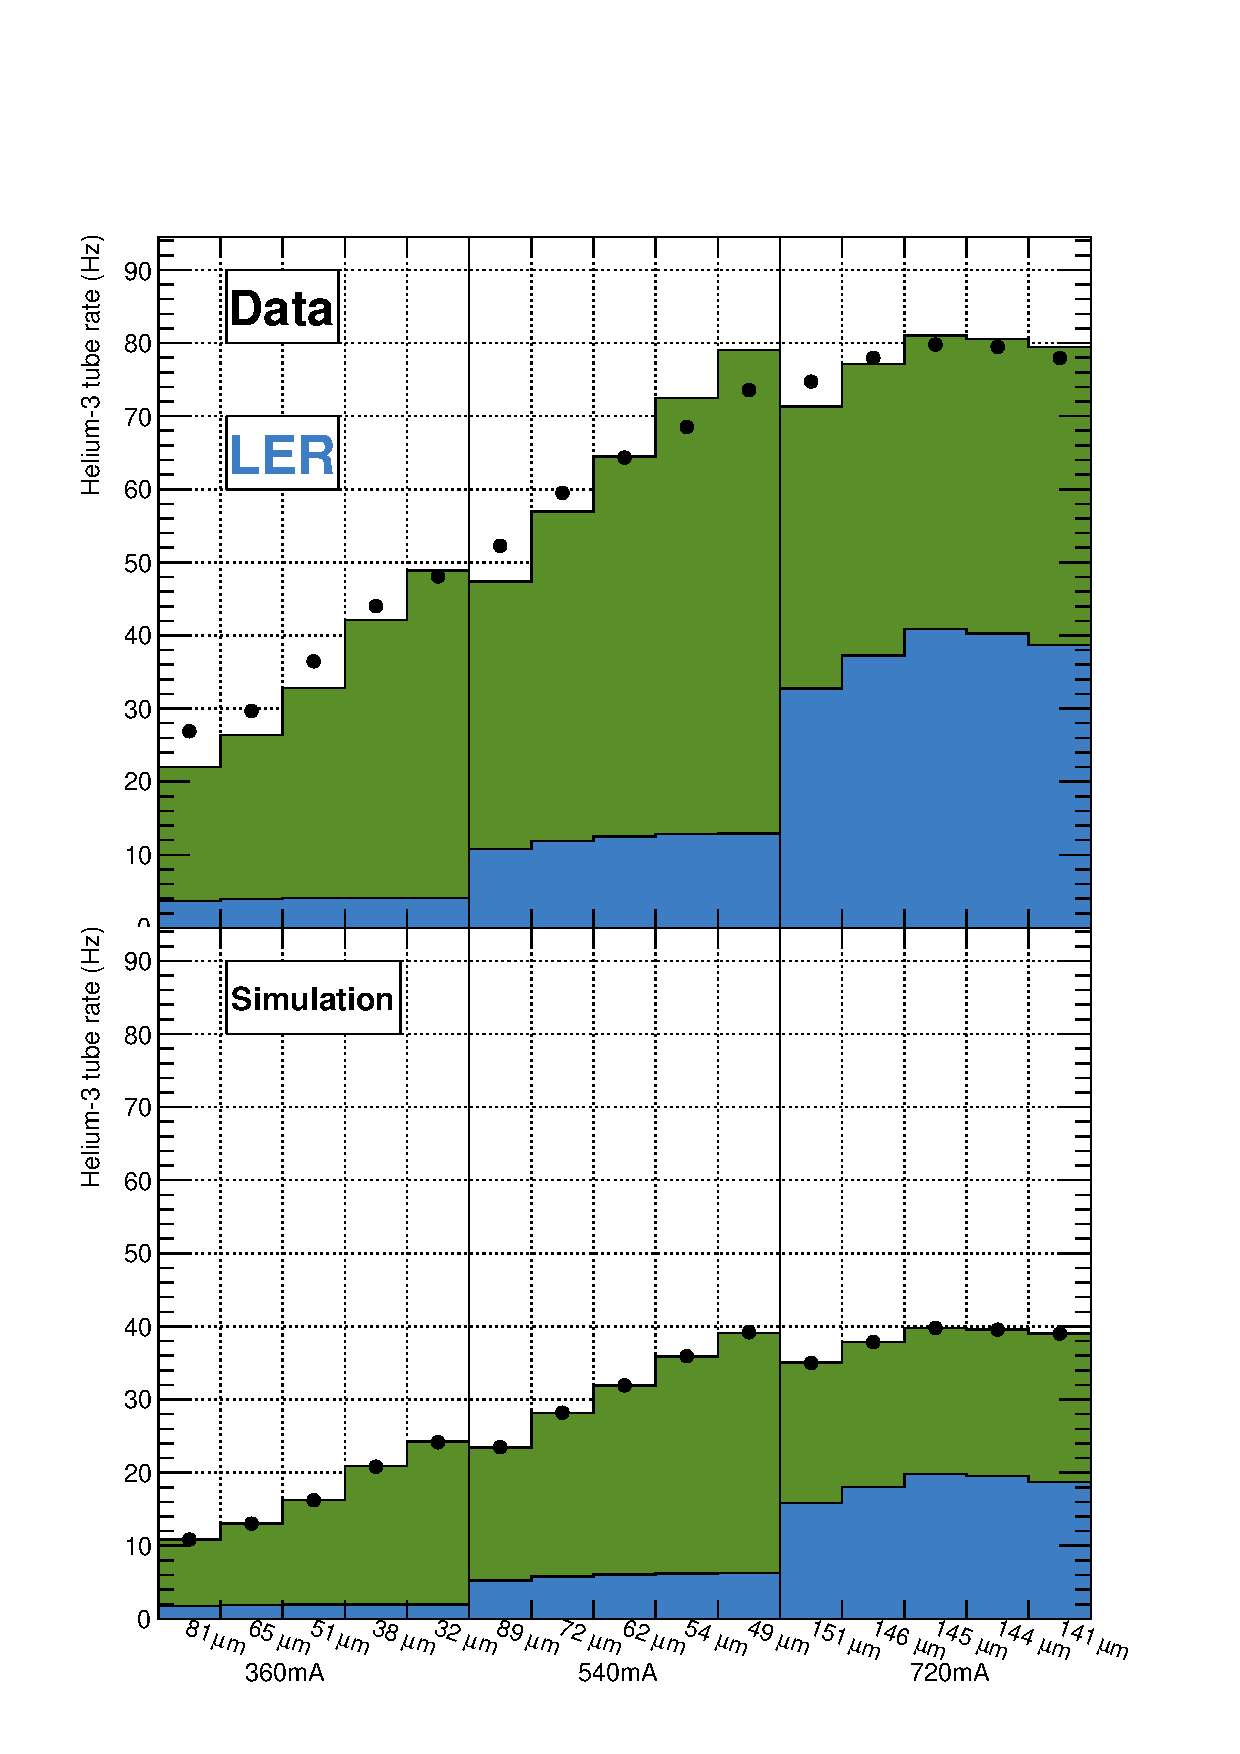
\includegraphics[width=\textwidth]{images/LERTousSecondPass_3}
		\begin{picture}(2,2)
			\put(-100,260){\thicklines\circle{10}}
			\put(-120,240){\thicklines\circle{10}}
			\put(-100,220){\thicklines\circle*{10}}
			\put(-80,240){\thicklines\circle{10}}
			\put(-104, 237){$\phi$}  
		\end{picture}
	\caption[Result of fit for Touschek experiments after simulation is weighted by $P_{\mathrm{scale}}$, LER, channel 3]{Result of fit for Touschek experiments after simulation is weighted by $P_{\mathrm{scale}}$, LER, channel 3. Green is the beam-beam component, blue is the beam-gas component, and black is the rate measured in \he tube channel 3. Error bars are the standard deviation of the mean of the rate in that bin and are too small to be seen on this scale.}	
	\label{fig:LERTous23}
\end{figure}


\begin{figure}
	\centerfloat
		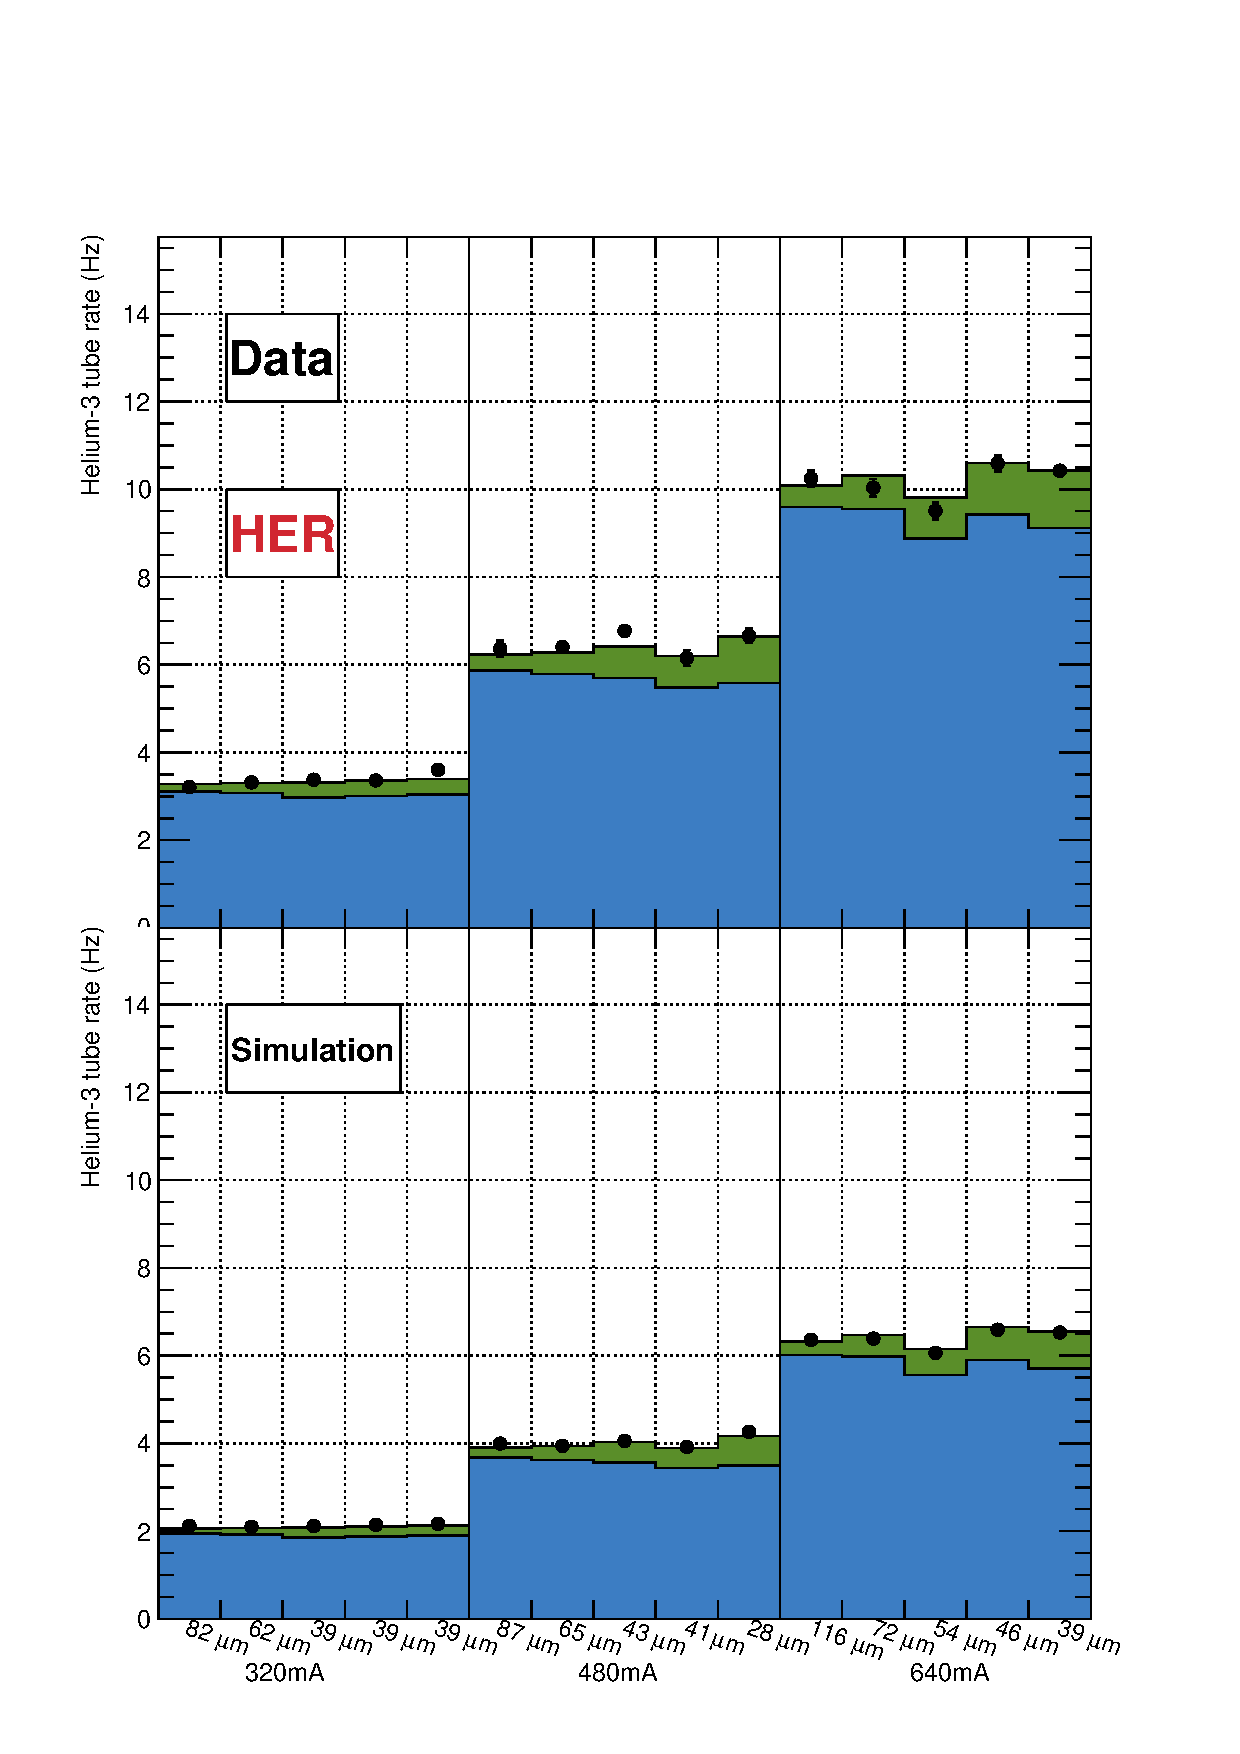
\includegraphics[width=\textwidth]{images/HERTousSecondPass_0}
		\begin{picture}(2,2)
			\put(-100,260){\thicklines\circle{10}} %1
			\put(-120,240){\thicklines\circle{10}}  %2
			\put(-100,220){\thicklines\circle{10}}  %3
			\put(-80,240){\thicklines\circle*{10}}   %0
			\put(-104, 237){$\phi$}  
		\end{picture}
	\caption[Result of fit for Touschek experiments after simulation is weighted by $P_{\mathrm{scale}}Z_{\mathrm{eff}}^{2}$, HER, channel 0]{Result of fit for Touschek experiments after simulation is weighted by $P_{\mathrm{scale}}Z_{\mathrm{eff}}^{2}$ , HER, channel 0. Green is the beam-beam component, blue is the beam-gas component, and black is the rate measured in \he tube channel 0. Error bars are the standard deviation of the mean of the rate in that bin and are too small to be seen on this scale.}	
	\label{fig:HERTous20}
\end{figure}

\begin{figure}
	\centerfloat
		\includegraphics[width=\textwidth]{images/HERTousSecondPass_1}
		\begin{picture}(2,2)
			\put(-100,260){\thicklines\circle*{10}} %1
			\put(-120,240){\thicklines\circle{10}}  %2
			\put(-100,220){\thicklines\circle{10}}  %3
			\put(-80,240){\thicklines\circle{10}}   %0
			\put(-104, 237){$\phi$}  
		\end{picture}
	\caption[Result of fit for Touschek experiments after simulation is weighted by $P_{\mathrm{scale}}Z_{\mathrm{eff}}^{2}$, HER, channel 1]{Result of fit for Touschek experiments after simulation is weighted by $P_{\mathrm{scale}}Z_{\mathrm{eff}}^{2}$ , HER, channel 1. Green is the beam-beam component, blue is the beam-gas component, and black is the rate measured in \he tube channel 1. Error bars are the standard deviation of the mean of the rate in that bin and are too small to be seen on this scale.}	
	\label{fig:HERTous21}
\end{figure}

\begin{figure}
	\centerfloat
		\includegraphics[width=\textwidth]{images/HERTousSecondPass_2}
		\begin{picture}(2,2)
			\put(-100,260){\thicklines\circle{10}} %1
			\put(-120,240){\thicklines\circle*{10}}  %2
			\put(-100,220){\thicklines\circle{10}}  %3
			\put(-80,240){\thicklines\circle{10}}   %0
			\put(-104, 237){$\phi$}  
		\end{picture}
	\caption[Result of fit for Touschek experiments after simulation is weighted by $P_{\mathrm{scale}}Z_{\mathrm{eff}}^{2}$, HER, channel 2]{Result of fit for Touschek experiments after simulation is weighted by $P_{\mathrm{scale}}Z_{\mathrm{eff}}^{2}$ , HER, channel 2. Green is the beam-beam component, blue is the beam-gas component, and black is the rate measured in \he tube channel 2. Error bars are the standard deviation of the mean of the rate in that bin and are too small to be seen on this scale.}	
	\label{fig:HERTous22}
\end{figure}

\begin{figure}
	\centerfloat
		\includegraphics[width=\textwidth]{images/HERTousSecondPass_3}
		\begin{picture}(2,2)
			\put(-100,260){\thicklines\circle{10}} %1
			\put(-120,240){\thicklines\circle{10}}  %2
			\put(-100,220){\thicklines\circle*{10}}  %3
			\put(-80,240){\thicklines\circle{10}}   %0
			\put(-104, 237){$\phi$}  
		\end{picture}
	\caption[Result of fit for Touschek experiments after simulation is weighted by $P_{\mathrm{scale}}Z_{\mathrm{eff}}^{2}$, HER, channel 3]{Result of fit for Touschek experiments after simulation is weighted by $P_{\mathrm{scale}}Z_{\mathrm{eff}}^{2}$ , HER, channel 3. Green is the beam-beam component, blue is the beam-gas component, and black is the rate measured in \he tube channel 3. Error bars are the standard deviation of the mean of the rate in that bin and are too small to be seen on this scale.}	
	\label{fig:HERTous23}
\end{figure}





	In order to verify the overall accuracy of the simulation, a ratio of the data to simulation for the beam-gas and Touschek parameters is defined:
\begin{subequations}
\begin{align}
		{(D/S)_{\mathrm{gas}} = c_{\mathrm{gas}}^{\mathrm{data}}/c_{\mathrm{gas}}^{\mathrm{sim}}} \\
		{(D/S)_{\mathrm{T}} = c_{\mathrm{T}}^{\mathrm{data}}/c_{\mathrm{T}}^{\mathrm{sim}}}
\end{align}
\end{subequations}
where $(D/S)_{\mathrm{gas}}$ is the data to simulation ratio for beam-gas, and $(D/S)_{\mathrm{T}}$ is the data to simulation ratio for Touschek.

The more accurate the simulation, the closer these ratios will be to 1. These ratios can also be used to scale the simulation to better match the data. The values of these ratios can be found in Table~\ref{tab:dataSimRatio}. Note that the table omits the uncertainty on the ratio. This is discussed in detail in \S~\ref{sec:Systematics}.

\begin{table}[htb]
	\centering
	\begin{tabular}{ ccc }
		& $(D/S)_{\mathrm{T}}$	&  $(D/S)_{\mathrm{gas}}$	\\ \hline \hline
	LER	& 2.153		& 2.188	\\ 
	HER	& 1.905		& 1.319	\\ \hline 
	\end{tabular}
	\caption[Ratio of data to simulation for beam-gas and Touschek parameters]{Ratio of data to simulation for beam-gas and Touschek parameters.}
	\label{tab:dataSimRatio}
\end{table}

\subsection{Systematic Uncertainties in Touschek Experiments}
\label{sec:Systematics}


	In order to get the uncertainty on $(D/S)_{gas}$ and $(D/S)_{T}$, it is necessary to determine the uncertainty on the beam current, beam size, $P_{\mathrm{scale}}Z_{\mathrm{eff}}^{2}$, and the \he tube efficiencies used in the simulation.

\paragraph{Uncertainty on beam current}
	
	The beam current is known to quite a high level of precision. The uncertainty on the current does not depend on the current, and is estimated to be 0.03~mA \cite{HiroEmailCurrentError}.


\paragraph{Uncertainty on beam size}
	
	The distribution of the beam size for HER and LER during the beam size scans is shown in Fig~\ref{fig:BeamSizeError}. To estimate the uncertainty on the beam size, the distributions are fit to Gaussian functions. The mean and sigma of the fits can be found in Table~\ref{tab:beamSizeGausFits}. For the HER, the uncertainty on the beam size is estimated to be 3.71\%. For the LER, the beam size uncertainty is estimated to be 1.37\%.


\begin{figure}
	\centering
	\subfigure{
		\begin{overpic}[trim={0 0 0 0.75cm},clip, width=\textwidth]{images/LERBeamSize}
		\end{overpic}
		\label{fig:LERBeamSizeError}
	}
	\subfigure{
		\begin{overpic}[trim={0 0 0 0.75cm},clip, width=\textwidth]{images/HERBeamSize}
		\end{overpic}
		\label{fig:HERBeamSizeError}
	}
	\caption[Estimation of beam size uncertainty]{Estimation of beam size uncertainty. Measurements were taken from the X-ray beam size monitor during beam size scans. The different colours indicate different subruns.}	
	\label{fig:BeamSizeError}
\end{figure}


\begin{table}[htb]
	\centering
	\begin{tabular}{ lllll }
		& Colour in Fig~\ref{fig:BeamSizeError}	& mean ($\mu m$)	& $\sigma$ ($\mu m$) & $\sigma$/mean	\\ \hline \hline
	LER	& Grey	& 81.02$\pm$0.10	& 1.30$\pm$0.09	    	& 0.0161	\\
		& Green	& 65.20$\pm$0.06	& 0.77$\pm$0.05	    	& 0.0114	\\ \hline
	HER	& Grey	& 86.96$\pm$0.23	& 3.19$\pm$0.23	    	& 0.0367	\\
		& Red	& 41.84$\pm$0.07	& 1.56$\pm$0.05	    	& 0.0372	\\
		& Blue	& 28.18$\pm$0.07    	& 1.06$\pm$0.05	& 0.0375	\\ \hline
	\end{tabular}
	\caption[Fit parameters for beam size distributions]{Fit parameters for beam size distributions.}
	\label{tab:beamSizeGausFits}
\end{table}


\paragraph{Uncertainty on $P_{\mathrm{s}}$$_{\mathrm{c}}$$_{\mathrm{a}}$$_{\mathrm{l}}$$_{\mathrm{e}}$$Z$$_{\mathrm{e}}^2$$_{\mathrm{f}}$$_{\mathrm{f}}$}

	The value of $P_{\mathrm{scale}}Z_{\mathrm{eff}}^{2}$ is calculated by averaging over the four \he tubes. To estimate the uncertainty, this parameter is calculated separately for each tube (see Table~\ref{tab:PScaleZsq}). The RMS of the four values is used as the uncertainty. These values can be found in Table~\ref{tab:PscaleZUncertainy}

\begin{table}[htb]
	\centering
	\begin{tabular}{ lSS }
		& {$P_{\mathrm{scale}}Z_{\mathrm{eff}}^{2}$}	& {RMS of $P_{\mathrm{scale}}Z_{\mathrm{eff}}^{2}$}	\\ \hline \hline
	HER	& 96.27	& 22.7	 \\
	LER	& 0.950	& 0.071 \\ \hline
	\end{tabular}
	\caption[RMS of $P_{\mathrm{scale}}Z_{\mathrm{eff}}^{2}$]{RMS of $P_{\mathrm{scale}}Z_{\mathrm{eff}}^{2}$.}
	\label{tab:PscaleZUncertainy}
\end{table}

\paragraph{Uncertainty on \He Tube Efficiency}

	The total uncertainty for each \he tube given in Table~\ref{tab:he3Calib} is used as the uncertainty on the \he tube efficiency.

\paragraph{Estimating the Uncertainty on $(D/S)$}

To estimate the systematic uncertainty from beam current, beam size, $P_{\mathrm{scale}}Z_{\mathrm{eff}}^{2}$, and \he tube efficiency, the simulation was re-weighted with each quantity separately adjusted to +1$\sigma$ and -1$\sigma$ values. The full analysis was then redone. For example:
\begin{subequations}
\begin{align}
		{I\rightarrow I+0.03\mathrm{~mA}} \\
		{I\rightarrow I-0.03\mathrm{~mA}}
\end{align}
\end{subequations}
and similarly for $\sigma_{y}$, $P_{\mathrm{scale}}$Z$^{2}$, and the \he tube efficiency. The analysis described in \S~\ref{sec:TousExp} was repeated to get new values of $R_{gas}$ and $R_{T}$. These are used to calculate the systematic error for each quantity:
\begin{subequations}
\begin{align}
	{\sigma_{(D/S)_{\mathrm{T}}+}^{I} = (D/S)_{\mathrm{T}}|_{I=I+0.03\mathrm{~mA}} - (D/S)_{\mathrm{T}}|_{\mathrm{nominal}}} \\
	{\sigma_{(D/S)_{\mathrm{T}}-}^{I} = (D/S)_{\mathrm{T}}|_{\mathrm{nominal}} - (D/S)_{\mathrm{T}}|_{I=I-0.03\mathrm{~mA}} }
\end{align}
\end{subequations}

Figure~\ref{fig:RatioWithErrors} shows the systematic uncertainty produced by each parameter. Table~\ref{tab:RatioWithErrors} contains the numerical values of these uncertainties. The uncertainty associated with $\phi$ is the standard deviation of the mean of the ratio for each of the four \he tubes, which are located at different $\phi$ positions around the beampipe. It is therefore a measure of how well the simulation predicts the $\phi$ distribution of the neutron flux.

\begin{table}[htb]
	\centering
	\begin{tabular}{ cSSSS }
	&	\multicolumn{2}{c}{Touschek}			&	\multicolumn{2}{c}{Beam-Gas}			\\	\hline \hline
LER	&	$\sigma_{+}$	&	$\sigma_{-}$	&	$\sigma_{+}$	&	$\sigma_{-}$	\\	
$P_{\mathrm{scale}}$	&	0.00084	&	0.00084	&	0.18	&	0.15	\\	
$\sigma_{y}$	&	0.028	&	0.028	&	0.	&	0.	\\	
I	&	0.00032	&	0.00032	&	0.000086	&	0.000086	\\	
$\phi$	&	0.27	&	0.27	&	0.35	&	0.35	\\	
$\varepsilon_{^3\mathrm{He}}$	&	0.21	&	0.18	&	0.21	&	0.18	\\	\hline
Total	&	0.34	&	0.33	&	0.44	&	0.42	\\	\hline
HER	&	$\sigma_{+}$	&	$\sigma_{-}$	&	$\sigma_{+}$	&	$\sigma_{-}$	\\	
$P_{\mathrm{scale}}Z^2$	&	0.24	&	0.19	&	0.41	&	0.25	\\	
$\sigma_{y}$	&	0.037	&	0.036	&	0.	&	0.	\\	
I	&	0.00018	&	0.00018	&	0.000076	&	0.000076	\\	
$\phi$	&	0.39	&	0.39	&	0.21	&	0.27	\\	
$\varepsilon_{^3\mathrm{He}}$	&	0.29	&	0.21	&	0.20	&	0.14	\\	\hline
Total	&	0.54	&	0.48	&	0.50	&	0.40	\\	\hline


	\end{tabular}
	\caption[Uncertainty contribution to $(D/S)$ from sources of systematic errors]{Uncertainty contribution to $(D/S)$ from sources of systematic errors. The values of (D/S) are given in Table~\ref{tab:dataSimRatio}.}
	\label{tab:RatioWithErrors}
\end{table}

\begin{figure}
	\centering
	\subfigure{
		\begin{overpic}[width=\textwidth]{images/LERRatioPlot}
		\end{overpic}
		\label{fig:LERRatioErrors}
	}
	\subfigure{
		\begin{overpic}[width=\textwidth]{images/HERRatioPlot}
		\end{overpic}
		\label{fig:HERRatioErrors}
	}
	\caption[LER and HER data simulation ratios with systematic errors]{LER and HER data simulation ratios with systematic errors. Blue is the beam-gas ratio, green is the Touschek ratio.}	
	\label{fig:RatioWithErrors}
\end{figure}

	The total uncertainty shown in Table~\ref{tab:RatioWithErrors} is the sum in quadrature of the uncertainty from each separate component. The major contributor to the uncertainty on the data/simulation ratio is the uncertainty due to the tubes being at different $\phi$ locations. This uncertainty is associated with the difference between the measured and simulated neutron flux at each different \he tube. A large uncertainty here shows that the simulation is incorrectly predicting the $\phi$ dependency of the neutron flux.


%------------------------------------------------------------------------------------------------

\subsection{Summary}

As shown in Tables~\ref{tab:dataSimRatio} and~\ref{tab:RatioWithErrors}, the ratio of data to simulation with uncertainties in the LER is 2.18$^{+0.44}_{-0.42}$ for beam-gas and 2.15$^{+0.34}_{-0.33}$ for Touschek, and in the HER is 1.32$^{+0.56}_{-0.36}$ for beam-gas and 1.91$^{+0.54}_{-0.48}$ for Touschek. The beam-gas LER-HER difference is $\pm2\sigma$, and the Touschek LER-HER difference is $\pm1\sigma$. Using these values, it is possible to re-scale the full Belle~II simulation to estimate what the neutron flux will actually be in Belle~II. This is discussed in Chapter~\ref{chap:Conseqences}.























%\chapter{Results}
\label{chap:Results}



\section{Touschek Studies}

\subsection{HER}

	Touschek effect not obvious in HER data.


\begin{figure}[htb]
	\centerfloat
		\includegraphics[trim={0 0 0 0.75cm},clip, scale=0.6]{images/2006}
	\caption{Rate in Helium-3 tubes vs HER inverse beam size at a current of 160mA}	
	\label{fig:TousHER2006}
\end{figure}

\begin{figure}[htb]
	\centerfloat
		\includegraphics[trim={0 0 0 0.75cm},clip, scale=0.6]{images/2007}
	\caption{Rate in Helium-3 tubes vs HER inverse beam size at a current of 320mA}	
	\label{fig:TousHER2007}
\end{figure}

\begin{figure}[htb]
	\centerfloat
		\includegraphics[trim={0 0 0 0.75cm},clip, scale=0.6]{images/2008}
	\caption{Rate in Helium-3 tubes vs HER inverse beam size at a current of 480mA}	
	\label{fig:TousHER2008}
\end{figure}

\begin{figure}[htb]
	\centerfloat
		\includegraphics[trim={0 0 0 0.75cm},clip, scale=0.6]{images/2009}
	\caption{Rate in Helium-3 tubes vs HER inverse beam size at a current of 640mA}	
	\label{fig:TousHER2009}
\end{figure}

\begin{figure}[htb]
	\centerfloat
		\includegraphics[scale=0.6]{images/HER_beamSize}
	\caption{HER Touschek contribution}	
	\label{fig:TousHERContrib}
\end{figure}

\clearpage

\subsection{LER}

\begin{figure}[htb]
	\centerfloat
		\includegraphics[trim={0 0 0 0.75cm},clip, scale=0.6]{images/12009}
	\caption{Rate in Helium-3 tubes vs LER inverse beam size at a current of 180mA}	
	\label{fig:TousLER12009}
\end{figure}

\begin{figure}[htb]
	\centerfloat
		\includegraphics[trim={0 0 0 0.75cm},clip, scale=0.6]{images/13006}
	\caption{Rate in Helium-3 tubes vs LER inverse beam size at a current of 360mA}	
	\label{fig:TousLER13006}
\end{figure}

\begin{figure}[htb]
	\centerfloat
		\includegraphics[trim={0 0 0 0.75cm},clip, scale=0.6]{images/13007}
	\caption{Rate in Helium-3 tubes vs LER inverse beam size at a current of 540mA}	
	\label{fig:TousLER13007}
\end{figure}


\begin{figure}[htb]
	\centerfloat
		\includegraphics[trim={0 0 0 0.75cm},clip, scale=0.6]{images/13008}
	\caption{Rate in Helium-3 tubes vs LER inverse beam size at a current of 720mA}	
	\label{fig:TousLER13008}
\end{figure}


\begin{figure}[htb]
	\centerfloat
		\includegraphics[trim={0 0 0 0.75cm},clip, scale=0.6]{images/13009}
	\caption{Rate in Helium-3 tubes vs LER inverse beam size at a current of 900mA}	
	\label{fig:TousLER13009}
\end{figure}


\begin{figure}[htb]
	\centerfloat
		\includegraphics[trim={0 0 0 0.75cm},clip, scale=0.6]{images/13010}
	\caption{Rate in Helium-3 tubes vs LER inverse beam size at a current of 1000mA}	
	\label{fig:TousLER13010}
\end{figure}

\begin{figure}[htb]
	\centerfloat
		\includegraphics[scale=0.6]{images/LER_beamSize2}
	\caption{LER Touschek contribution}	
	\label{fig:TousLERContrib}
\end{figure}


\clearpage

\section{Vacuum Bump Studies}



\subsection{HER}

	No RGA data for HER.
	Is the double bump observed?

\subsection{LER}

	only have RGA data for run 5002.
	





\chapter{Consequences for the Belle~II Experiment}
\label{chap:Conseqences}

	Simulations of the expected neutron flux in full Belle~II running at the design luminosity of 8$\times10^{35}$ cm$^{-2}$s$^{-1}$ with residual gas pressure of 10~nTorr were calculated using SAD to simulate collider conditions and GEANT4 to simulate the detector. Table \ref{tab:neutronFluxTable} shows the highest neutron flux expected in each subdetector, as predicted by SAD and GEANT4. Figures showing the expected neutron flux in each subdetector can be found in Figs~\ref{fig:VXDFlux}-\ref{fig:EKLMForFlux}.


\begin{table}[ht]
	\centering
	\begin{tabular}{ lSSSS }	
	&	{Maximum}	&		&	{Maximum}	&		\\	
	&	{Neutron Flux}	&		&	{Neutron Flux}	&		\\	
	&	{No Re-weighting}	&	{Tolerance}	&	 {After Re-weighting}	&		\\	
Subdetector	&	{($\times10^{9}$cm$^{-2}$yr$^{-1}$)} 	&	{($\times10^{9}$cm$^{-2}$yr$^{-1}$)} 	&	{($\times10^{9}$cm$^{-2}$yr$^{-1}$)}	&	{\% increase}	\\	\hline \hline
PXD	&	92	&		&	106	&	15.7	\\	
SVD	&	373	&		&	421	&	12.9	\\	
CDC	&	57	&	100	&	70	&	23.0	\\	
ARICH	&	104	&	100	&	115	&	9.8	\\	
TOP – Bars	&	46	&	50	&	56	&	19.7	\\	
TOP – Electronics	&	16	&		&	21	&	28.5	\\	
ECL - Forward	&	23	&	100	&	24	&	3.8	\\	
ECL - Barrel	&	5	&	100	&	6	&	26.2	\\	
ECL - Backward	&	14	&	100	&	19	&	36.0	\\	
BKLM	&	0.37	&		&	0.46	&	23.6	\\	
EKLM - Forward	&	1.88	&		&	2.26	&	20.0	\\	
EKLM - Backward	&	1.56	&		&	1.72	&	10.8	\\	\hline

	\end{tabular}
	\caption[Neutron flux as predicted by SAD and GEANT4]{Neutron flux as predicted by SAD and GEANT4.}
	\label{tab:neutronFluxTable}
\end{table}




Using the parameters $(D/S)_{\mathrm{gas}}$ and $(D/S)_{\mathrm{T}}$ described in \S~\ref{sec:TousExp}, the beam-gas and Touschek components of these simulations can be re-weighted to improve the prediction of the neutron flux. The Belle~II subdetector most affected by the re-weighting of the beam-gas and Touschek simulation is the backward part of the ECL. Fortunately, the predicted neutron flux, though increased, is still well below the tolerance. There are four different background components: Touschek, beam-gas, and two radiative Bhabha components. Only the Touschek and beam-gas components can be re-weighted at this time. The TOP and ARICH, while showing smaller increases, are both slightly outside their tolerances, as shown in Fig \ref{fig:increasePlot}. The average increase for all subdetectors is $\sim$20\%, which is a significant increase. Further thought must be given to mitigating this higher than expected neutron flux, such as additional neutron shielding. It might also be necessary to replace components as they become too irradiated.


Since there were no collisions in Phase~I, there is no information on the radiative Bhabha backgrounds, and they can not be re-weighted at this time. The cross section for this process is well understood, and does not require simulation of the collider with SAD. It does, however, require GEANT4 simulation. This will assist in determining whether SAD or GEANT4 is the source of the discrepancy between data and simulation.



%Although the cross section for this process is well understood, which reduces the uncertainty from this background, the source of neutron production induced by this process still relies on GEANT4 simulation of Belle~II. 


\begin{figure}[htb]
	\centerfloat
		\includegraphics[width=\textwidth]{images/hVXDFlux}
	\caption[Neutron flux in VXD]{Neutron flux in VXD. Layers 1 \& 2 are the PXD and 3-6 are the SVD.}	
	\label{fig:VXDFlux}
\end{figure}

\begin{figure}[htb]
	\centerfloat
		\includegraphics[width=\textwidth]{images/hCDCFlux}
	\caption[Neutron flux in CDC electronics]{Neutron flux in CDC electronics. Layer 1 is the innermost layer. Larger layer numbers correspond to higher radii.}	
	\label{fig:CDCFlux}
\end{figure}

\begin{figure}[htb]
	\centerfloat
		\includegraphics[width=\textwidth]{images/hARICHFlux}
	\caption[Neutron flux in ARICH rings]{Neutron flux in ARICH Rings. Ring-ID of 1 is the innermost ring. Ring-ID increases with radius.}	
	\label{fig:ARICHFlux}
\end{figure}

\begin{figure}[htb]
	\centerfloat
		\includegraphics[width=\textwidth]{images/hTOPFlux}
	\caption[Neutron flux in TOP electronics]{Neutron flux in TOP electronics.}	
	\label{fig:TOPFlux}
\end{figure}

\begin{figure}[htb]
	\centerfloat
		\includegraphics[width=\textwidth]{images/hTOPFluxBar}
	\caption[Neutron flux in TOP quartz bars]{Neutron flux in TOP quartz bars.}	
	\label{fig:TOPBARFlux}
\end{figure}

\begin{figure}[htb]
	\centerfloat
		\includegraphics[width=\textwidth]{images/hECLFluxTID}
	\caption[Neutron flux in ECL diodes]{Neutron flux in ECL diodes. Explanation of $\theta_{ID}$ can be found in Appendix \ref{chap:THID}.}	
	\label{fig:ECLFlux}
\end{figure}

\begin{figure}[htb]
	\centerfloat
		\includegraphics[width=\textwidth]{images/hBKLMFlux}
	\caption[Neutron flux in BKLM]{Neutron flux in BKLM. Layer 1 is the innermost layer. Layer increases with radius.}	
	\label{fig:BKLMFlux}
\end{figure}

\begin{figure}[htb]
	\centerfloat
		\includegraphics[width=\textwidth]{images/hEKLMFlux}
	\caption[Neutron flux in EKLM]{Neutron flux in EKLM. Negative layers are backward end-cap, positive layers are forward end-cap. Layers 1 and -1 are closest to IR.}	
	\label{fig:EKLMForFlux}
\end{figure}



\begin{figure}
	\centerfloat
		\includegraphics[width=\textwidth]{images/IncreasePlot}
	\caption[Increase in background flux in each detector]{Increase in background flux in each detector.}
	\label{fig:increasePlot}
\end{figure}






























\chapter{Conclusion}
\label{chap:Concl}



The studies described here show that the simulated flux of neutrons from beam-gas and Touschek interactions are underestimating the actual neutron flux by 2.18$^{+0.44}_{-0.42}$ and 2.15$^{+0.34}_{-0.33}$ for beam-gas and Touschek on the LER respectively, and 1.32$^{+0.56}_{-0.36}$ and 1.91$^{+0.54}_{-0.48}$ for beam-gas and Touschek on the HER respectively. The ramification of this is that Belle~II will experience a 20\% higher than expected total neutron flux for these sources. The detectors will have a neutron flux at a higher rate than was initially expected and some detectors will have a neutron flux above their tolerance.

When Phase~II of BEAST~II runs, there will be collisions, which will allow the radiative Bhabha component of the backgrounds to be measured. The \he tubes will be present at this time and thus the neutron rate due to these Bhabhas can be measured for comparison with the simulation.

During Belle~II's physics running, the Belle~II detector will trigger data acquisition at random times when the beams are being circulated. This will allow for real time measurement of beam backgrounds. It is likely that one or more of the \he tubes will be used to measure the neutron flux during the full Belle~II experiment, as a monitor on the neutron flux from the beam backgrounds.









% The style of bibliography exemplified here is the "plain",
% normally used in science theses. This is shown
% by the entry {plain} below. Substitute the
% appropriate bibliography style. See also the
% PDF file "InformationOnBibliographyStyles" in this
% directory for more choices.

% The Bibliography file is a BibTex file named
% UVicThesis.bib and called below

	\TOCadd{Bibliography}
	\bibliographystyle{unsrt}
	\bibliography{References}


	\appendix

%\chapter{Americium-Beryllium Neutron Energy Spectrum}
\label{chap:AmBeSpec}

\begin{figure}[htb]
	\centerfloat
		\includegraphics[scale=0.6]{images/AmBe_NeutronSpectrum.pdf}
	\caption[Energy spectrum of neutrons from AmBe source]{Energy spectrum of neutrons from AmBe source~\cite{AmBeSpec}.}
	\label{fig:AmBeSpec}
\end{figure}

%\chapter{Systematic errors on \He tube efficiency}
\label{chap:calibUn}

\begin{table}[htb]
	\centering
	\begin{tabular}{ lrrr }
			&	All points		&	First 5 points		&	Last 7 points		\\	\hline \hline
	B		&	7.243	$\times10^{6}cm^2s^{-1}$	&	11.237	$\times10^{6}cm^2s^{-1}$	&	2.391	$\times10^{6}cm^2s^{-1}$	\\	
$	r_{0}	$	&	0.400	cm	&	-7.862	cm	&	49.086	cm	\\	
	C		&	107.856	Hz	&	148.731	Hz	&	133.724	Hz	\\	
$	A_{0}	$	&	0.278		&	0.194		&	0.340		\\	
$	A_{1}	$	&	0.282		&	0.203		&	0.341		\\	
$	A_{2}	$	&	0.154		&	0.115		&	0.184		\\	
$	A_{3}	$	&	0.201		&	0.148		&	0.240		\\	
$	A_{Sim}	$	&	1.000		&	1.000		&	1.000		\\	
$	C_{2}	$	&	100.455	Hz	&	-86.851	Hz	&	154.101	Hz	\\	\hline

	\end{tabular}
	\caption{Fit parameters for calibration fits}
	\label{tab:CalibrationFitPars}
\end{table}




\begin{figure}
	\centering
	\subfigure[First 5 points only]{
		\begin{overpic}[width=\textwidth]{images/first5points}
		\end{overpic}
		\label{fig:he3rateVsDfirst5}
	}
	\subfigure[Last 7 points only]{
		\begin{overpic}[width=\textwidth]{images/last7points}
		\end{overpic}
		\label{fig:he3rateVsDlast7}
	}
	\caption{\He tube rate vs distance from thermal neutron source, reduced points}
	\label{fig:he3rateVsDReduced}
\end{figure}

%\chapter{Data Tables}
\label{chap:miscData}








\begin{table}[htb]
	\centering
	\begin{tabular}{ cccccc }
		&	& \multicolumn{2}{c}{Data}		& \multicolumn{2}{c}{Simulation}	\\
		& & c$_{gas}$	& c$_{T}$	& c$_{gas}$	& c$_{T}$	\\ 
		&Channel &  [$Hz/(mA\cdot Pa)$]	& [$Hz\cdot\mu m/mA^{2}$]	& [$Hz/(mA\cdot Pa)$]	& [$Hz\cdot\mu m/mA^{2}$]\\ \hline \hline
	LER	& 0	& 6320$\pm$80	& 16.60$\pm$0.09& 3188.4$\pm$0.4& 8.1949$\pm$0.0005		\\
		& 1	& 3290$\pm$60	& 8.19$\pm$0.06	& 2438.5$\pm$0.3& 5.1703$\pm$0.0004		\\
		& 2	& 5640$\pm$70	& 13.53$\pm$0.08& 1939.4$\pm$0.3& 4.7398$\pm$0.0003		\\
		& 3	& 7950$\pm$80	& 18.27$\pm$0.09& 2949.9$\pm$0.4& 6.5233$\pm$0.0004		\\ \hline	
	HER	& 0& (240$\pm$4)$\times10^{3}$& 0.23$\pm$0.03	& 1732.2$\pm$1.1& 0.200570$\pm$0.000007		\\ 
		& 1& (109$\pm$3)$\times10^{3}$& 0.11$\pm$0.02	& 1274.9$\pm$0.8& 0.095905$\pm$0.000006		\\
		& 2& (178$\pm$4)$\times10^{3}$& 0.18$\pm$0.03	& 1022.7$\pm$0.7& 0.092316$\pm$0.000005		\\
		& 3& (239$\pm$4)$\times10^{3}$& 0.23$\pm$0.03	& 1688.1$\pm$1.1& 0.192070$\pm$0.000008		\\ \hline
	\end{tabular}
	\caption{Fit parameters associated with figs \ref{fig:LERTous10}, \ref{fig:LERTous11}, \ref{fig:LERTous12}, \ref{fig:LERTous13}, and \ref{fig:HERTous10}, \ref{fig:HERTous11}, \ref{fig:HERTous12}, \ref{fig:HERTous13}}
	\label{tab:FirstPassFitPars}
\end{table}

\begin{table}[htb]
	\centering
	\begin{tabular}{ cccc }
		&	& \multicolumn{2}{c}{Simulation} \\	
		& 	& c$_{gas}$	& c$_{T}$	\\ 
		&Channel &  [$Hz/(mA\cdot Pa)$]	& [$Hz\cdot\mu m/mA^{2}$]\\ \hline \hline
	LER	&0	& 3028.2$\pm$0.4& 8.1928$\pm$0.0005\\
		&1	& 2316.0$\pm$0.3& 5.1687$\pm$0.0003		\\
		&2	& 1842.0$\pm$0.2& 4.7385$\pm$0.0003		\\
		&3	& 2801.7$\pm$0.4& 6.5214$\pm$0.0004		\\ \hline	
	HER	&0	& (167$\pm$0.11)$\times10^{3}$& 0.1527$\pm$0.0008	\\
		&1	& (123$\pm$0.08)$\times10^{3}$& 0.0590$\pm$0.0006	\\
		&2	& (99$\pm$0.07)$\times10^{3}$ & 0.0621$\pm$0.0005	\\
		&3	& (163$\pm$0.11)$\times10^{3}$& 0.1432$\pm$0.0008	\\ \hline
	\end{tabular}
	\caption[Fit parameters associated with figs \ref{fig:LERTous20}, \ref{fig:LERTous21}, \ref{fig:LERTous22}, \ref{fig:LERTous23} and \ref{fig:HERTous20}, \ref{fig:HERTous21}, \ref{fig:HERTous22}, \ref{fig:HERTous23}]{Fit parameters associated with figs \ref{fig:LERTous20}, \ref{fig:LERTous21}, \ref{fig:LERTous22}, \ref{fig:LERTous23} and \ref{fig:HERTous20}, \ref{fig:HERTous21}, \ref{fig:HERTous22}, \ref{fig:HERTous23}. Data fits are the same as in table \ref{tab:FirstPassFitPars}}
	\label{tab:SecondPassFitPars}
\end{table}



%
\chapter{Neutron Flux in Belle~II subdetectors}
\label{chap:NFluxBelle}

\begin{figure}[htb]
	\centerfloat
		\includegraphics[width=\textwidth]{images/hVXDFlux}
	\caption[Neutron flux in VXD]{Neutron flux in VXD. Layers 1 \& 2 are the PXD and 3-6 are the SVD.}	
	\label{fig:VXDFlux}
\end{figure}

\begin{figure}[htb]
	\centerfloat
		\includegraphics[width=\textwidth]{images/hCDCFlux}
	\caption[Neutron flux in CDC electronics]{Neutron flux in CDC electronics. Layer 1 is the innermost layer. Larger layer numbers correspond to higher radii.}	
	\label{fig:CDCFlux}
\end{figure}

\begin{figure}[htb]
	\centerfloat
		\includegraphics[width=\textwidth]{images/hARICHFlux}
	\caption[Neutron flux in ARICH rings]{Neutron flux in ARICH Rings. Ring-ID of 1 is the innermost ring. Ring-ID increases with radius.}	
	\label{fig:ARICHFlux}
\end{figure}

\begin{figure}[htb]
	\centerfloat
		\includegraphics[width=\textwidth]{images/hTOPFlux}
	\caption{Neutron flux in TOP electronics.}	
	\label{fig:TOPFlux}
\end{figure}

\begin{figure}[htb]
	\centerfloat
		\includegraphics[width=\textwidth]{images/hTOPFluxBar}
	\caption{Neutron flux in TOP quartz bars.}	
	\label{fig:TOPBARFlux}
\end{figure}

\begin{figure}[htb]
	\centerfloat
		\includegraphics[width=\textwidth]{images/hECLFluxTID}
	\caption[Neutron flux in ECL diodes]{Neutron flux in ECL diodes. Explanation of $\theta_{ID}$ can be found in Appendix \ref{chap:THID}.}	
	\label{fig:ECLFlux}
\end{figure}

\begin{figure}[htb]
	\centerfloat
		\includegraphics[width=\textwidth]{images/hBKLMFlux}
	\caption[Neutron flux in BKLM]{Neutron flux in BKLM. Layer 1 is the innermost layer. Layer increases with radius.}	
	\label{fig:BKLMFlux}
\end{figure}

\begin{figure}[htb]
	\centerfloat
		\includegraphics[width=\textwidth]{images/hEKLMFlux}
	\caption[Neutron flux in EKLM]{Neutron flux in EKLM. Negative layers are backward end-cap, positive layers are forward end-cap. Layers 1 and -1 are closest to IR.}	
	\label{fig:EKLMForFlux}
\end{figure}

%\begin{figure}[htb]
%	\centerfloat
%		\includegraphics[scale=0.6]{images/BelleIIFlux}
%	\caption{Flux in the Belle~II detector}	
%	\label{fig:BelleIIFlux}
%\end{figure}



\chapter{$\theta_{I}$$_{D}$ of ECL}
\label{chap:THID}


A brief explanation of the parameter $\theta_{ID}$ is necessary, since many of the plots presented here use it as an axis, instead of $\theta$. $\theta_{ID}$ is a value assigned to each ring of crystals, starting from 0 for the first ring of crystals in the forward end-cap of the ECL, and ending at 68 for the last ring of crystals in the backward end-cap. A visual explanation of this is shown in Fig~\ref{fig:thetaID}. $\theta_{ID}$ values from 0-12 are in the forward end-cap, 13-58 are in the barrel, and 59-68 are in the backward end-cap. 

\begin{figure}[htb]
	\centerfloat
		\includegraphics[scale=0.7]{images/ThetaID}
	\caption[$\theta_{ID}$ values for ECL]{$\theta_{ID}$ values for ECL.}	
	\label{fig:thetaID}
\end{figure}


\chapter{\He Tube specifications and circuit diagrams}
\label{chap:he3spec}

\begin{sidewaysfigure}
	\centering
		\includegraphics[width=\paperwidth]{images/He3Schematic}
	\caption[\He tube schematic]{\He tube schematic (used with permission)~\cite{GEREUTER}.}
	\label{fig:he3spec}
\end{sidewaysfigure}

\begin{sidewaysfigure}
	\centering
		\includegraphics[width=\paperwidth]{images/PCB}
	\caption[\He tube detector preamp HV PCB]{\He tube detector preamp HV PCB~\cite{Honkanen}.}
	\label{fig:he3HVPCB}
\end{sidewaysfigure}


\begin{sidewaysfigure}
	\centering
		\includegraphics[width=\paperwidth]{images/linedrive}
	\caption[\He tube detector preamp with line driver]{\He tube detector preamp with line driver~\cite{Honkanen}.}
	\label{fig:he3preampLineDriver}
\end{sidewaysfigure}

\begin{sidewaysfigure}
	\centering
		\includegraphics[width=\paperwidth]{images/linerecieve}
	\caption[\He tube detector line receiver]{\He tube detector line receiver~\cite{Honkanen}.}
	\label{fig:he3LineReciever}
\end{sidewaysfigure}






\end{document}
